\documentclass{llncs}
\usepackage{graphicx}
%\usepackage{lineno}
\usepackage{color}
\usepackage{amsmath}
\usepackage{amssymb}
\usepackage{xspace}
%\usepackage{amsthm}
\usepackage{url}
\usepackage{hyperref}

\usepackage{cite}
%additional packages
\usepackage{epsfig}
\usepackage{subfigure}
\usepackage{fancybox}
\usepackage{algorithmic}
\usepackage{mathstyle}
\usepackage{amstext}
\usepackage{graphicx}
\usepackage{tabularx}
\usepackage{color}
\usepackage{multirow}

\graphicspath{{Figures/}}

\newcommand\defeq{\stackrel{\mathrm{def}}{=}}
% Add a period to the end of an abbreviation unless there's one
% already, then \xspace.
\makeatletter
\DeclareRobustCommand\onedot{\futurelet\@let@token\@onedot}
\def\@onedot{\ifx\@let@token.\else.\null\fi\xspace}

\newcommand{\yasu}[1]{\textcolor{red}{{[Yasu: #1]}}}

\def\eg{\emph{e.g}\onedot} \def\Eg{\emph{E.g}\onedot}
\def\ie{\emph{i.e}\onedot} \def\Ie{\emph{I.e}\onedot}
\def\cf{\emph{c.f}\onedot} \def\Cf{\emph{C.f}\onedot}
\def\etc{\emph{etc}\onedot} \def\vs{\emph{vs}\onedot} 
\def\wrt{w.r.t\onedot} \def\dof{d.o.f\onedot}
\def\etal{\emph{et al}\onedot}

\newcommand{\figcaption}[1]{\def\@captype{figure}\caption{#1}}
\newcommand{\tblcaption}[1]{\def\@captype{table}\caption{#1}}
\makeatother

\newcommand{\argmax}{\operatornamewithlimits{argmax}}
\newcommand{\argmin}{\operatornamewithlimits{argmin}}


\newcommand{\skewsym}[1] {[#1]_{\times}}

\newcommand{\bth}    {\mbox{\boldmath $\theta$}}
\newcommand{\bdth}   {\mbox{\boldmath $\dot{\theta}$}}
\newcommand{\bddth}  {\mbox{\boldmath $\ddot{\theta}$}}
\newcommand{\blam}   {\mbox{\boldmath $\lambda$}}
\newcommand{\bXi}    {\mbox{\boldmath $\Xi$}}
\newcommand{\bUps}   {\mbox{\boldmath $\Upsilon$}}
\newcommand{\btau}   {\mbox{\boldmath $\tau$}}
\newcommand{\bsigma} {\mbox{\boldmath $\sigma$}}
\newcommand{\bPsi}   {\mbox{\boldmath $\Psi$}}
\newcommand{\bOm}    {\mbox{\boldmath $\Omega$}}
\newcommand{\bom}    {\mbox{\boldmath $\omega$}}

\newcommand{\vdr} {\boldsymbol{\dot{r}}}
\newcommand{\mdJ} 	{\boldsymbol{\dot{J}}}
\newcommand{\mdA} 	{\boldsymbol{\dot{A}}}

\newcommand{\vsigma} {\boldsymbol{\sigma}}
\newcommand{\veta} {\boldsymbol{\eta}}
\newcommand{\vom} {\boldsymbol{\omega}}
\newcommand{\vup} {\boldsymbol{\upsilon}}
\newcommand{\vrho} {\boldsymbol{\rho}}
\newcommand{\vkappa} {\boldsymbol{\kappa}}
\newcommand{\vxi} {\boldsymbol{\xi}}
\newcommand{\vgamma} {\boldsymbol{\gamma}}
\newcommand{\mGamma} {\boldsymbol{\Gamma}}
\newcommand{\mPhi} {\boldsymbol{\Phi}}
\newcommand{\mPsi} {\boldsymbol{\Psi}}

\newcommand {\mat}[1] {{\bf #1}}

\newcommand{\mA} {\mat{A}}
\newcommand{\mB} {\mat{B}}
\newcommand{\mC} {\mat{C}}
\newcommand{\mD} {\mat{D}}
\newcommand{\mE} {\mat{E}}
\newcommand{\mF} {\mat{F}}
\newcommand{\mG} {\mat{G}}
\newcommand{\mH} {\mat{H}}
\newcommand{\mI} {\mat{I}}
\newcommand{\mJ} {\mat{J}}
\newcommand{\mK} {\mat{K}}
\newcommand{\mM} {\mat{M}}
\newcommand{\mR} {\mat{R}}
\newcommand{\mP} {\mat{P}}
\newcommand{\mS} {\mat{S}}
\newcommand{\mT} {\mat{T}}


\newcommand \Ad     {\mathrm{Ad}}
\newcommand \ad     {\mathrm{ad}}
\newcommand \se     {\mathrm{se}}
\newcommand \SE     {\mathrm{SE}}

\newcommand{\bAB}{\mbox{\boldmath$AB$}}
\newcommand{\bAC}{\mbox{\boldmath$AC$}}
\newcommand{\bAF}{\mbox{\boldmath$AF$}}
\newcommand{\bAO}{\mbox{\boldmath$AO$}}
\newcommand{\bAP}{\mbox{\boldmath$AP$}}
\newcommand{\bAZ}{\mbox{\boldmath$AZ$}}
\newcommand{\bBF}{\mbox{\boldmath$BF$}}
\newcommand{\bBZ}{\mbox{\boldmath$BZ$}}
\newcommand{\bCF}{\mbox{\boldmath$CF$}}
\newcommand{\bCG}{\mbox{\boldmath$CG$}}
\newcommand{\bCP}{\mbox{\boldmath$CP$}}
\newcommand{\bDG}{\mbox{\boldmath$DG$}}
\newcommand{\bDP}{\mbox{\boldmath$DP$}}
\newcommand{\bFB}{\mbox{\boldmath$FB$}}
\newcommand{\bFC}{\mbox{\boldmath$FC$}}
\newcommand{\bFG}{\mbox{\boldmath$FG$}}
\newcommand{\bFO}{\mbox{\boldmath$FO$}}
\newcommand{\bFP}{\mbox{\boldmath$FP$}}
\newcommand{\bGA}{\mbox{\boldmath$GA$}}
\newcommand{\bGOF}{\mbox{\boldmath$G_1F$}}
\newcommand{\bGG}{\mbox{\boldmath$GG$}}
\newcommand{\bGH}{\mbox{\boldmath$GH$}}
\newcommand{\bGL}{\mbox{\boldmath$GL$}}
\newcommand{\bGPG}{\mbox{\boldmath$G'G$}}
\newcommand{\bGJ}{\mbox{\boldmath$GJ$}}
\newcommand{\bGO}{\mbox{\boldmath$GO$}}
\newcommand{\bGOOO}{\mbox{\boldmath$G_1O_1$}}
\newcommand{\bGP}{\mbox{\boldmath$GP$}}
\newcommand{\bGPP}{\mbox{\boldmath$G'P$}}
\newcommand{\bGOP}{\mbox{\boldmath$G_1P$}}
\newcommand{\bGR}{\mbox{\boldmath$GR$}}
\newcommand{\bGS}{\mbox{\boldmath$GS$}}
\newcommand{\bGPS}{\mbox{\boldmath$G'S$}}
\newcommand{\bJK}{\mbox{\boldmath$JK$}}
\newcommand{\bJH}{\mbox{\boldmath$JH$}}
\newcommand{\bOA}{\mbox{\boldmath$OA$}}
\newcommand{\bOF}{\mbox{\boldmath$OF$}}
\newcommand{\bOG}{\mbox{\boldmath$OG$}}
\newcommand{\bOM}{\mbox{\boldmath$OM$}}
\newcommand{\bOO}{\mbox{\boldmath$OO$}}
\newcommand{\bOP}{\mbox{\boldmath$OP$}}
\newcommand{\bOS}{\mbox{\boldmath$OS$}}
\newcommand{\bOZ}{\mbox{\boldmath$OZ$}}
\newcommand{\bPG}{\mbox{\boldmath$PG$}}
\newcommand{\bPK}{\mbox{\boldmath$PK$}}
\newcommand{\bPO}{\mbox{\boldmath$PO$}}
\newcommand{\bZB}{\mbox{\boldmath$ZB$}}
\newcommand{\bZC}{\mbox{\boldmath$ZC$}}
\newcommand{\bZG}{\mbox{\boldmath$ZG$}}
\newcommand{\bZO}{\mbox{\boldmath$ZO$}}


\newcommand{\ab}{\mbox{$\mathbf{A_b}$}}
\newcommand{\bA}{\mbox{\boldmath $A$}}
\newcommand{\bB}{\mbox{\boldmath $B$}}
\newcommand{\bC}{\mbox{\boldmath $C$}}
\newcommand{\bD}{\mbox{\boldmath $D$}}
\newcommand{\bE}{\mbox{\boldmath $E$}}
\newcommand{\bF}{\mbox{\boldmath $F$}}
\newcommand{\bG}{\mbox{\boldmath $G$}}
\newcommand{\bH}{\mbox{\boldmath $H$}}
\newcommand{\bI}{\mbox{\boldmath $I$}}
\newcommand{\bJ}{\mbox{\boldmath $J$}}
\newcommand{\bK}{\mbox{\boldmath $K$}}
\newcommand{\bL}{\mbox{\boldmath $L$}}
\newcommand{\bl}{\mbox{\boldmath $l$}}
\newcommand{\bM}{\mbox{\boldmath $M$}}
\newcommand{\bN}{\mbox{\boldmath $N$}}
\newcommand{\bP}{\mbox{\boldmath $P$}}
\newcommand{\bO}{\mbox{\boldmath $O$}}
\newcommand{\bQ}{\mbox{\boldmath $Q$}}
\newcommand{\bR}{\mbox{\boldmath $R$}}
\newcommand{\bS}{\mbox{\boldmath $S$}}
\newcommand{\bT}{\mbox{\boldmath $T$}}
\newcommand{\bU}{\mbox{\boldmath $U$}}
\newcommand{\bV}{\mbox{\boldmath $V$}}
\newcommand{\bW}{\mbox{\boldmath $W$}}
\newcommand{\bd}{\mbox{\boldmath $d$}}
\newcommand{\bff}{\mbox{\boldmath $f$}}
\newcommand{\bg}{\mbox{\boldmath $g$}}
\newcommand{\ba}{\mbox{\boldmath $a$}}
\newcommand{\bb}{\mbox{\boldmath $b$}}
\newcommand{\bc}{\mbox{\boldmath $c$}}
\newcommand{\be}{\mbox{\boldmath $e$}}
\newcommand{\bh}{\mbox{\boldmath $h$}}
\newcommand{\bk}{\mbox{\boldmath $k$}}
\newcommand{\bm}{\mbox{\boldmath $m$}}
\newcommand{\bn}{\mbox{\boldmath $n$}}
%\newcommand{\bnA}{\mbox{\boldmath ${n_A}$}}
\newcommand{\bp}{\mbox{\boldmath $p$}}
\newcommand{\bq}{\mbox{\boldmath $q$}}
\newcommand{\bx}{\mbox{\boldmath $x$}}
\newcommand{\br}{\mbox{\boldmath $r$}}
\newcommand{\bdq}{\mbox{\boldmath $\dot{q}$}}
\newcommand{\bu}{\mbox{\boldmath $u$}}
%\newcommand{\bv}{\mbox{\boldmath $v$}}
\newcommand{\bzero}{\mbox{\boldmath $0$}}
\newcommand{\bim}{\mbox{\boldmath $\imath$}}
\newcommand{\bjm}{\mbox{\boldmath $\jmath$}}
\newcommand{\bxk}{\mbox{\boldmath ${x_k}$}}
\newcommand{\marktodoag}[1]{\colorbox{yellow}{#1}}      % needs \usepackage{color}
\newcommand{\marktododo}[1]{\colorbox{cyan}{#1}}        % needs \usepackage{color}
\newenvironment{comment}{\mbox{}\textbf{\marktodoag{Comment:}} }{}


\newcommand{\vddth} {\boldsymbol{\ddot{\theta}}}
\newcommand{\sv} {{\bf v}} %spatial vector v
\newcommand{\vth} {\boldsymbol{\theta}}
\newcommand{\SO} {\mathsf{SO(3)}}
\newcommand{\dse} {\mathsf{se^\ast(3)}}
\newcommand{\dAd} {\mathsf{Ad^\ast}}
\newcommand{\real} {\mathbb{R}}
\newcommand{\eye} {\mathbf{1}}
\newcommand{\vdth} {\boldsymbol{\dot{\theta}}}

% Down from ORIN

\newcommand{\Bfor}{{\bf for}}
\newcommand{\Bforall}{{\bf for all}}
\newcommand{\Bto}{{\bf to}}
\newcommand{\Bwhile}{{\bf while}}
\newcommand{\Beach}{{\bf each}}
\newcommand{\Bdo}{{\bf do}}
\newcommand{\Bif}{{\bf if}}
\newcommand{\Bthen}{{\bf then}}
\newcommand{\Bend}{{\bf end}}
\newcommand{\Bendfor}{{\bf end for}}

\newenvironment{program}{\begin{tabbing}
\hspace{.2in}\=\+%
\hspace{.2in}\=\hspace{.2in}\=\hspace{.2in}\=%
\hspace{.2in}\=\hspace{.2in}\=\hspace{.2in}\=\kill}%
{\end{tabbing}}

\newenvironment{pbox}[1]{\begin{parbox}[t]{2.67 in %6.25 cm
}{#1\\}}{\end{parbox}}

\newcommand{\strutUp}{\rule[-0.6ex]{0ex}{2.8ex}}     % for use in tables
\newcommand{\strutDown}{\rule[-1.0ex]{0ex}{2.8ex}}

\newcommand{\bigsum}[1]{
\sum_{\parbox[c]{0.8cm}{ \scriptsize \vspace{-4.0ex}
\begin{displaymath} #1 \end{displaymath} } } }

\newcommand{\ms}{m^*}
\newcommand{\vc}{\vec{c}}
\newcommand{\vg}{\vec{g}}
\newcommand{\vcs}{\vc^*}
\newcommand{\vcds}{\dot{\vc}^*}
\newcommand{\vp}{\vec{p}}
\newcommand{\vpd}{\dot{\vp}}
\newcommand{\vI}{\vec{I}}
\newcommand{\vIb}{\bar{\vI}}
\newcommand{\vIbs}{\vIb^*}
\newcommand{\vk}{\vec{k}}
\newcommand{\vtheta}{\vec{\theta}}
\newcommand{\vthetad}{\dot{\vtheta}}
\newcommand{\Gs}{G^*}
\newcommand{\vr}{\vec{r}}
\newcommand{\vrs}{\vr^*}
\newcommand{\vrds}{\dot{\vr}^*}

\newcommand{\BM}{\begin{bmatrix}}
\newcommand{\EM}{\end{bmatrix}}
\newcommand{\EQ}{\!\!\!{=}\!\!\!}   % for use in eqnarray environment
\newcommand{\vecarrow}[1]{{\stackrel{\longrightarrow}{#1}}}

\newcommand{\valpha}{\vec{\alpha}}
\newcommand{\vbeta}{\vec{\beta}}
\newcommand{\bbeta}{\mbox{\boldmath$\beta$}}
\newcommand{\vdelta}{\vec{\delta}}
\newcommand{\vepsilon}{\vec{\epsilon}}
\newcommand{\epsilond}{\dot{\epsilon}}
\newcommand{\vzeta}{\vec{\zeta}}
\newcommand{\bzeta}{\mbox{\boldmath$\zeta$}}
\newcommand{\bvartheta}{\mbox{\boldmath$\vartheta$}}
\newcommand{\vLambda}{\vec{\Lambda}}
\newcommand{\vlambda}{\vec{\lambda}}
\newcommand{\blambda}{\mbox{\boldmath$\lambda$}}
%\newcommand{\vmu}{\vec{\mu}}
\newcommand{\bmu}{\mbox{\boldmath$\mu$}}
\newcommand{\brho}{\mbox{\boldmath$\rho$}}
\newcommand{\vtau}{\vec{\tau}}
% \newcommand{\btau}{\mbox{\boldmath$\tau$}}
\newcommand{\uvtau}{\underline{\vtau}}
\newcommand{\vPhi}{\vec{\Phi}}
\newcommand{\vPhid}{\dot{\vPhi}}
\newcommand{\bPhid}{\dot{\bPhi}}
\newcommand{\vPhic}{\mathring{\vPhi}}
\newcommand{\vphi}{\vec{\phi}}
\newcommand{\bPhi}{{\bf \Phi}}
\newcommand{\vPsi}{\vec{\Psi}}
\newcommand{\vomega}{\vec{\omega}}
\newcommand{\uvomega}{\underline{\vomega}}

%\newcommand{\bzero}{{\bf 0}}
\newcommand{\ubzero}{\underline{\bzero}}
\newcommand{\bone}{{\bf 1}}
\newcommand{\vzero}{{\vec{0}}}
\newcommand{\vone}{{\vec{1}}}

\newcommand{\vA}{\vec{A}}
\newcommand{\va}{\vec{a}}
%\newcommand{\ba}{{\bf a}}
\newcommand{\uva}{\underline{\va}}
\newcommand{\uba}{\underline{\ba}}
%\newcommand{\bA}{{\bf A}}
\newcommand{\vB}{\vec{B}}
\newcommand{\vb}{\vec{b}}
%\newcommand{\bb}{{\bf b}}
\newcommand{\uvb}{\underline{\vb}}
\newcommand{\vC}{\vec{C}}
%\newcommand{\bC}{{\bf C}}
\newcommand{\Cqt}{\vC\,\bqd+\btau_g}
%\newcommand{\bc}{{\bf c}}
\newcommand{\uvc}{\underline{\vc}}
\newcommand{\vD}{\vec{D}}
\newcommand{\dd}[2]{\frac{{\rm d}#1}{{\rm d}#2}}
\newcommand{\ldd}[2]{{\rm d}#1/{\rm d}#2}
\newcommand{\ddt}{\dd{}{t}}
\newcommand{\diag}{{\rm diag}}
\newcommand{\vd}{\vec{d}}
%\newcommand{\bd}{{\bf d}}
\newcommand{\EE}{{\sf E}}
\newcommand{\vE}{\vec{E}}
%\newcommand{\be}{{\bf e}}
\newcommand{\FF}{{\sf F}}
\newcommand{\vF}{\vec{F}}
%\newcommand{\bF}{{\bf F}}
\newcommand{\vf}{\vec{f}}
\newcommand{\Bf}{{\bf f}}
\newcommand{\uvf}{\underline{\vf}}
\newcommand{\ubf}{\underline{\Bf}}
%\newcommand{\bfJ}[1]{\Bf_{{\scriptscriptstyle\rm J}#1}}
\newcommand{\bfJ}[1]{\Bf_{#1}^J}
\newcommand{\vG}{\vec{G}}
%\newcommand{\bg}{{\bf g}}
\newcommand{\vh}{\vec{h}}
\newcommand{\vdh} {\dot{\vec{h}}}
\newcommand{\vH}{\vec{H}}
%\newcommand{\bH}{{\bf H}}
%\newcommand{\bh}{{\bf h}}
\newcommand{\vHd}{\dot{\bf H}}
\newcommand{\bhd}{\dot{\bf h}}
%\newcommand{\bI}{{\bf I}}
\newcommand{\ID}{I\!D}
\newcommand{\vIbar}{\bar{\vI}}
\newcommand{\vJ}{\vec{J}}
%\newcommand{\bJ}{{\bf J}}
\newcommand{\vK}{\vec{K}}
\newcommand{\vdk} {\dot{\vec{k}}}
\newcommand{\vL}{\vec{L}}
\newcommand{\vl}{\vec{l}}
\newcommand{\vdl} {\dot{\vec{l}}}
%\newcommand{\bl}{{\bf l}}
\newcommand{\MM}{{\sf M}}
\newcommand{\vM}{\vec{M}}
%\newcommand{\bm}{{\bf m}}
\newcommand{\uvm}{\underline{\vm}}
\newcommand{\ubm}{\underline{\bm}}
\newcommand{\vn}{\vec{n}}
\newcommand{\uvn}{\underline{\vn}}
\newcommand{\vP}{\vec{P}}
\newcommand{\vdp} {\dot{\vec{p}}}
%\newcommand{\bP}{{\bf P}}
\newcommand{\uvp}{\underline{\vp}}
\newcommand{\Pos}[2]{{}^{#1}\!\vp_{#2}}
\newcommand{\uPos}[2]{{}^{#1}\!\uvp_{#2}}
%\newcommand{\bp}{{\bf p}}
\newcommand{\vq}{\vec{q}}
%\newcommand{\bq}{{\bf q}}
\newcommand{\vqd}{\dot{\vq}}
\newcommand{\vdq} {\dot{\vec{q}}}
\newcommand{\bqd}{\dot{\bq}}
\newcommand{\vqdd}{\ddot{\vq}}
\newcommand{\vddq} {\ddot{\vec{q}}}
\newcommand{\bqdd}{\ddot{\bq}}
\newcommand{\qd}{\dot{q}}
\newcommand{\qdd}{\ddot{q}}
\newcommand{\range}{{\rm Range}}
\newcommand{\rank}{{\rm rank}}
\newcommand{\vR}{\vec{R}}
\newcommand{\Rot}[2]{{}^{#1}\!\vR_{#2}}
\newcommand{\RR}{{\sf R}}
\newcommand{\uvr}{\underline{\vr}}
\newcommand{\vS}{\vec{S}}
\newcommand{\Bs}{{\bf s}}
\newcommand{\ubs}{\underline{\Bs}}
\newcommand{\bsd}{\dot{\Bs}}
\newcommand{\vT}{\vec{T}}
\newcommand{\vU}{\vec{U}}
\newcommand{\vu}{\vec{u}}
%\newcommand{\bu}{{\bf u}}
\newcommand{\vv}{\vec{v}}
\newcommand{\bv}{{\bf v}}
\newcommand{\bvJ}[1]{\bv_{#1}^J}
\newcommand{\uvv}{\underline{\vv}}
\newcommand{\ubv}{\underline{\bv}}
\newcommand{\vX}{\vec{X}}
\newcommand{\bX}{{\bf X}}
\newcommand{\XJ}{{\vX\!_J}}
\newcommand{\XL}{{\vX\!_L}}
\newcommand{\XF}[2]{{}^{#1}\!\vX_{\!#2}^F}
\newcommand{\XM}[2]{{}^{#1}\!\vX_{\!#2}}
\newcommand{\cX}[2]{{}^{#1}\!{\cal X}_{\!#2}}
\newcommand{\vx}{\vec{x}}
\newcommand{\vy}{\vec{y}}
\newcommand{\vz}{\vec{z}}
\newcommand{\hx}{\hat{\vx}}
\newcommand{\hy}{\hat{\vy}}
\newcommand{\hz}{\hat{\vz}}


% Up from ORIN





%\newtheorem{prop}{Proposition}
%\newtheorem{prf}{Proof}

\def\title#1{{\noindent\Large{\bf #1}\par}}
\def\author#1{\begin{center}{\sc #1\par}\end{center}}
%\renewcommand{\section}[1]{\vspace{0.1in}\noindent{\large\bf{#1}}\par\vspace{.05in}\par\nopagebreak}

\makeatletter
\def\thebibliography#1{\section{Recommended Readings\@mkboth
{REFERENCES}{REFERENCES}}\list
{[\arabic{enumi}]}{\settowidth\labelwidth{[#1]}\leftmargin\labelwidth
\advance\leftmargin\labelsep
\usecounter{enumi}}
\def\newblock{\hskip .11em plus .33em minus .07em}
\sloppy\clubpenalty4000\widowpenalty4000
\sfcode`\.=1000\relax}
\makeatother


\begin{document}


\pagestyle{empty}

\title{Momentum-Based Balance Control}
\author{Sung-Hee Lee, KAIST; Andreas Hofmann, MIT; Ambarish Goswami, Honda}

%%%%%%%%%%%%%%%%%%%%%%%%%%%%%%%%%%%%%%%%%%%%%%%%%%%%%%%%%%%%%%%%%%%%%%%%%%%%%%%
%%%%%%%%%%%%%%%%%%%%%%%%%%%%%%%%%%%%%%%%%%%%%%%%%%%%%%%%%%%%%%%%%%%%%%%%%%%%%%%
\section{Introduction}
%%%%%%%%%%%%%%%%%%%%%%%%%%%%%%%%%%%%%%%%%%%%%%%%%%%%%%%%%%%%%%%%%%%%%%%%%%%%%%%
%%%%%%%%%%%%%%%%%%%%%%%%%%%%%%%%%%%%%%%%%%%%%%%%%%%%%%%%%%%%%%%%%%%%%%%%%%%%%%%

%%%%%%%%%%%%%%%%%%%%%%%%%%%%%%%%%%%%%%%%%%%%%%%%%%%%%%%%%%%%%%%%%%%%%%%%%%%%%%%
%\subsection{What is momentum?}
%%%%%%%%%%%%%%%%%%%%%%%%%%%%%%%%%%%%%%%%%%%%%%%%%%%%%%%%%%%%%%%%%%%%%%%%%%%%%%%

%\subsection{Humanoid Robot Tasks and Their Specification}


% [To Do Andreas

% Add 2004 IROS reference, before ref. 29

% Need a better transition from Intro to Momentum section.
% In general, we need better transitions, and a better overview.

% Add journal paper reference?  Does this get too far into task stuff?
% Consult with Ambarish and Sung-Hee.

% Table 1 is useful.  Refer to it in my discussion?  In particular, Pd is silly.
% A key message of this paper should be that 1d is the right way to think about this problem.

% In section 2.1, I use the term ZMP, but this has not been introduced at this point.
% Should I just use P, to be consistent with the previous terminology?  Should we introduce
% ZMP first?  Section 2.1 should probably refer back to Table 1.  The ZMP control approach
% corresponds to Table 1a, the correct approach, 1d.

% Take out note in section 4.1.

% Is the notation in eqs. 20, 21 sufficiently consistent with the preceding analysis on how
% to compute momentum?  Fig. 6, in the preceding analysis, uses ``G'' to refer to CoM, whereas
% in section 4.1, I use ``CoM''.  I can change this to ``G'' to be consistent;  please advise.

% Do we need a separate definition of ZMP, distinct from ``P'' in the previous analysis?
% I can change the notation to ``P'', please advise.

% Use Centroidal Moment Pivot, not Point.

% ]


Humanoid bipedal morphologies have unique characteristics that provide significant advantages (and some disadvantages) over quadruped or wheeled robots. 
Key functional features of the humanoid morphology include a variable base of support and a high center of mass.
Because bipeds have only two legs, their support base is naturally constrained, allowing them to operate in environments where support base space is limited; 
many human environments require this. 
The legs can also be placed in wide stances, when space permits, enhancing stability against disturbances.
The feet can also be placed in specific locations, allowing for traversal over terrain where foot placement is constrained due to obstacles.
Thus, a key advantage of the humanoid morphology is that the variable base of support allows both for operation in constrained spaces, 
as well as stability against disturbances, 
Humanoid bipeds also have a high center of mass.  
This has the advantage that an elevated ``sensor package'' can be supported; when standing erect, the head can see over obstacles. 

An example task for such a system is to walk to a moving soccer ball and kick it, as shown in Figure \ref{fig:Soccer1}.  
Stepping movement must be synchronized with ball movement so that the kick happens when the ball is close enough.  
More generally, such tasks require that the biped be in an acceptable location and pose at an acceptable time.  
This implies spatial and temporal constraints for such tasks.  
There are also important dynamic balance constraints that limit the kinds of movements the biped may make without falling down.

\begin{figure}[b]
\centering
 \subfigure[]
    {
       \label{fig:SoccerKick}
       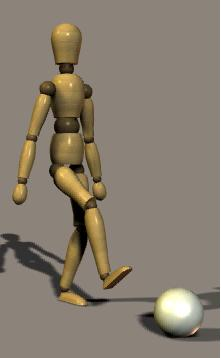
\includegraphics[height=1.5in]{SoccerKick}
    }
 \subfigure[]
   {
       \label{fig:SoccerTrip}
       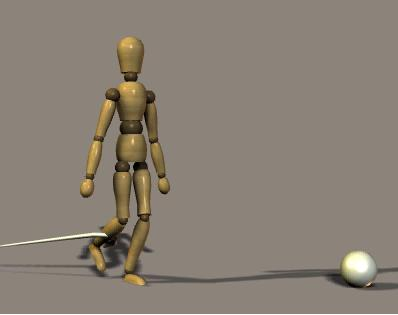
\includegraphics[height=1.5in]{SoccerTrip}
   }\vspace{-10pt}
\caption{Kicking soccer ball task, interrupted by trip disturbance}
\label{fig:Soccer1}
\end{figure}

If the system encounters a disturbance while performing a task, it will have to compensate in some way in order to satisfy these constraints.  
The disturbance may cause a delay, allowing another player to kick the ball, or it may interfere with movement synchronization.  
For example, a trip, shown in Figure \ref{fig:SoccerTrip} causes disruption of synchronization between the stepping foot, and the overall forward movement 
of the system’s center of mass. 

Another example task is walking on a constrained foot path, such as stones across a brook, or on a balance beam.  
As with the soccer ball example, this task has spatial, temporal, and dynamic constraints, but in this case, the spatial constraints are more stringent;  
the biped must reach its goal using foot placements that are precisely constrained. 
Figure \ref{fig:WalkOnStonesIntro1} shows a biped walking over blocks that constrain foot placement.  
When foot placement is constrained, the stepping pattern can’t be changed arbitrarily to compensate for a disturbance.  
For example, if a lateral push disturbance occurs, rather than stepping the leg out to the side, other compensating techniques, 
such as angular movement of the body and swing leg must be used, as shown in Figure \ref{fig:LatPushIntro1}.

\begin{figure}%[b]
\centering
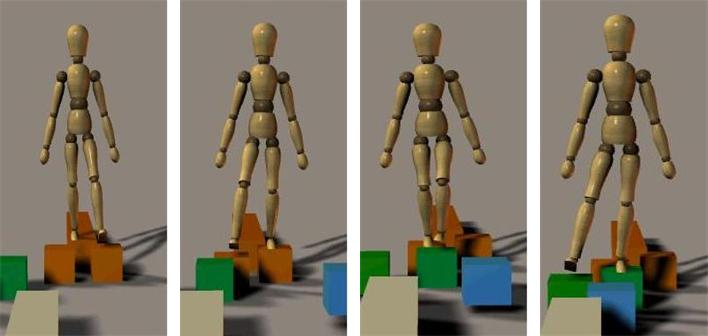
\includegraphics[height=1.5in]{WalkOnStonesIntro1}
\caption{Dynamic walking with foot placement constraints.}
\label{fig:WalkOnStonesIntro1}       
\end{figure}

\begin{figure}%[b]
\centering
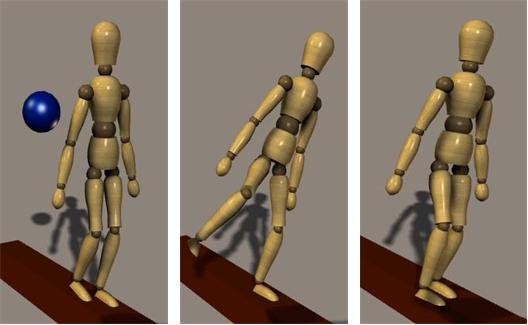
\includegraphics[height=1.5in]{LatPushIntro1}
\caption{Compensating for lateral push disturbance using angular movement of torso and swing leg.}
\label{fig:LatPushIntro1}       
\end{figure}



%%%%%%%%%%%%%%%%%%%%%%%%%%%%%%%%%%%%%%%%%%%%%%%%%%%%%%%%%%%%%%%%%%%%%%%%%%%%%%%
\subsection{Locomotion task execution for humanoid robots}
%%%%%%%%%%%%%%%%%%%%%%%%%%%%%%%%%%%%%%%%%%%%%%%%%%%%%%%%%%%%%%%%%%%%%%%%%%%%%%%

In the previously described examples, and others like them, the key challenge is to move the humanoid,
a complex, dynamic system, to an acceptable pose at an acceptable time, despite actuation limits, and despite disturbances.
The system should be able to recover from disturbances such as slips, trips, pushes, and ground contact instability due to soft terrain, 
even when foot placement is constrained.  
In particular, it should utilize flexibility in the task specification to achieve its goals.
For example, it may temporarily sacrifice a goal of maintaining an upright pose in order to achieve balance goals.

To achieve this, we seek to develop a robust plan execution system capable of guiding a robotic biped through a series of walking task goals, in the presence of disturbances.  
The system must understand commands at the task level;  it must take as input a high-level specification of where it should be, and by what time, and then 
automatically figure out the details of how to move to accomplish these goals.  
It should also be able to automatically detect whether a task that it is given can be accomplished in the allotted time, and should warn the human operator 
when this is not the case.  
If a disturbance occurs during execution of the task, the system should attempt to compensate in order to avoid a fall, and should still try to 
complete the task on time.  
If this is not possible, the system should alert the user, or a higher-level control authority, and should prepare itself for failure.
For example, if a fall is inevitable, it should put out its hands to break the fall.



%%%%%%%%%%%%%%%%%%%%%%%%%%%%%%%%%%%%%%%%%%%%%%%%%%%%%%%%%%%%%%%%%%%%%%%%%%%%%%%
\subsection{The role of momentum control in humanoid task execution}
%%%%%%%%%%%%%%%%%%%%%%%%%%%%%%%%%%%%%%%%%%%%%%%%%%%%%%%%%%%%%%%%%%%%%%%%%%%%%%%

A comprehensive discussion of humanoid task execution is beyond the scope of this chapter.
The reader is referred to previous work on this topic, particularly on task executives that utilize
spatial and temporal flexibility in the task specification \cite{hofmann2015temporally, hofmann2006exploiting}.
In this chapter, we will focus on momentum control, a foundational capability that supports
humanoid task execution.

Momentum control involves control of two major components:  linear, and angular.  
For both components, there are typically goals to control system momentum, as well as the momentum of 
individual links in the mechanism.
For example, for the linear component, there will typically be a goal to control the Center of Mass (CoM)
so that balance is maintained, and there may also be goals to control momentum of the feet to achieve
particular foot placements.
For the angular component, there will typically be a goal to minimize overall angular momentum
(and particularly, changes in overall angular momentum), in order to minimize energy losses \cite{PHH04}.
There will also typically be goals to maintain an upright posture of the torso and head.
As we will show, there are also interesting cases where rapid changes to overall angular momentum
are desirable.
These cases occur when linear momentum control becomes difficult (possibly due to a disturbance,
or limited foot placement options).  In such cases, the goal of minimal overall angular momentum
can be temporarily sacrificed so that the linear momentum control goal is achieved.



\subsubsection{Momentum Control Problem Definition and Challenges}

Before describing how momentum control works in detail, we first provide a definition
of what we mean by momentum control, within the context of task execution.

To begin, we use the term ``control'' here in a very general sense;
our use of this term does not necessarily imply stabililty or controllability as these terms are 
traditionally used in control theory.
Instead, we adopt a more practical definition, relevant to the goal of executing a task or set of tasks.
This is motivated by the fact that it is often sufficient to ``influence'' a quantity of interest, such as the 
forward momentum of the Center of Mass, even if strict linear controllability is not possible.
For example, it may be impossible to bring a fast running biped robot to a full stop in one single-support step,
but it may be possible to use a sequence of such steps to decelerate the robot until it stops.
This may or may not be acceptable, depending on the task state and temporal requirements.
For example, if the robot requires three steps to stop, but is one step from the edge of a cliff, the robot
does not have sufficient momentum controllability to avoid falling off the cliff.

Thus, the problem we address is implementation of a \textit{momentum controller} that provides 
\textit{sufficient momentum controllability}.
We define \textit{momentum controllability} to be sufficient if the momentum can be influenced 
enough to satisfy task requirements.

% What does it mean to control momentum in support of a task?
% Do we need more definition here?  This would require getting into task specifications, plan representations, etc.

This problem is challenging because, for a biped, momentum is influenced by interaction with the external environment,
through contact of the feet with the ground.
The amount of force that can be exerted this way is limited, due both to limitations of the biped's actuators, 
as well as the inherent limitations of exerting force on a relatively high CoM with a relatively narrow foot print.
Despite the serious actuation limits, bipeds are capable of achieving remarkable tasks like walking, running, and
jumping on restricted terrain, if they use an appropriate momentum controller.

Note that our definition of sufficient momentum controllability does not, necessarily, require stability in the 
traditional sense;
not all tasks for humanoid forms necessarily require balance as an end goal. 
For example, a football player trying to score a touchdown, or a baseball player trying to catch a fly ball,
does not care if he is upright at the end, as long as the goal is achieved.

This is a more useful definition than traditional concepts of balance control.
Such traditional concepts define successful balance control by the ability to 
accelerate the CoM sufficiently in any direction in the horizontal plane, so that the robot does not fall.
A fall is defined by contact of a non-foot link of the robot with the ground.
Such a balance control definition is adequate if the task goal is simply to stand in one place
(in double support or single support), and reject external balance disturbances.
Such a balance control definition also covers the concept of changing foot placement, by stepping,
to enhance momentum controllability.
Thus, the biped could, if pushed severely, take one or more steps to recover.
In fact, under this definition, in the absence of other task goals, it is ok for the CoM to move in random 
directions, as long as the stepping action of the feet provides a sufficient base of support to
beneficially accelerate the CoM so that the biped does not fall.
Note also that this traditional balance control definition is an infinite time concept, similar to the concept of 
stability for non-linear systems.

We believe that our definition is more practically useful.
We sidestep the difficult issue of infinite time stability and focus instead on the present and near future
goals, as expressed by state and temporal constraints in the task specification \cite{hofmann2015temporally}.
This often means balance control, as in the traditional definition, at least for the duration of the task,
but with additional constraints
for moving the CoM to an acceptable state, within an acceptable time, and with possible restrictions
on where the feet can be placed.

% Modify introductory paragraph in Section 4.1 to refer to this problem definition.


[Need overview paragraph, after momentum control section.]



%%%%%%%%%%%%%%%%%%%%%%%%%%%%%%%%%%%%%%%%%%%%%%%%%%%%%%%%%%%%%%%%%%%%%%%%%%%%%%%
\subsection{Momentum control}
%%%%%%%%%%%%%%%%%%%%%%%%%%%%%%%%%%%%%%%%%%%%%%%%%%%%%%%%%%%%%%%%%%%%%%%%%%%%%%%


Until recently, most balance control techniques
have attempted to maintain balance by controlling
only the linear motion of a robot.
For example, Kagami et al.~\cite{Kagami00} and
Kudoh et al.~\cite{Kudoh02} proposed methods to change
the input joint angle trajectories to modify the position of the
Center of Pressure (CoP), a point within the robot's support area through
which the resultant Ground Reaction Force (GRF) acts.
When the CoP, computed from the input joint motion, leaves the
support base, indicating a possible toppling of a foot,
the motion is modified to bring the CoP back inside the
support base while the robot still follows the desired linear
motion of the Center of Mass (CoM). The rotational motion of the
robot remains more or less ignored in these approaches.

However, rotational dynamics of a robot plays a
significant role in balance~\cite{KLKK05}.
%A control strategy narrowly focusing only on the linear CoM
%motion can inadvertently allow unnecessary and potentially harmful
%rotational motion of the robot.
%Previous balance controllers %that primarily focused on the linear motion of a robot
%avoided this problem somewhat heuristically, e.g.,
%by kinematically controlling the orientation of the trunk or
%by adding a specific joint space controller~\cite{Hyon07}.
%A more principled approach would be to control
%the robot's rotational dynamics directly. Indeed, e
Experiments on human balance control also show that
humans tightly regulate angular momentum during gait~\cite{PHH04},
which suggests the strong possibility that angular momentum
may be important in humanoid movements.

In fact, both angular and linear momenta
must be regulated to completely control the CoP. The fundamental quantities and the
relations between them are schematically depicted in Fig.~\ref{fig:one2one} and described subsequently.
\begin{figure}[h]
\begin{center}
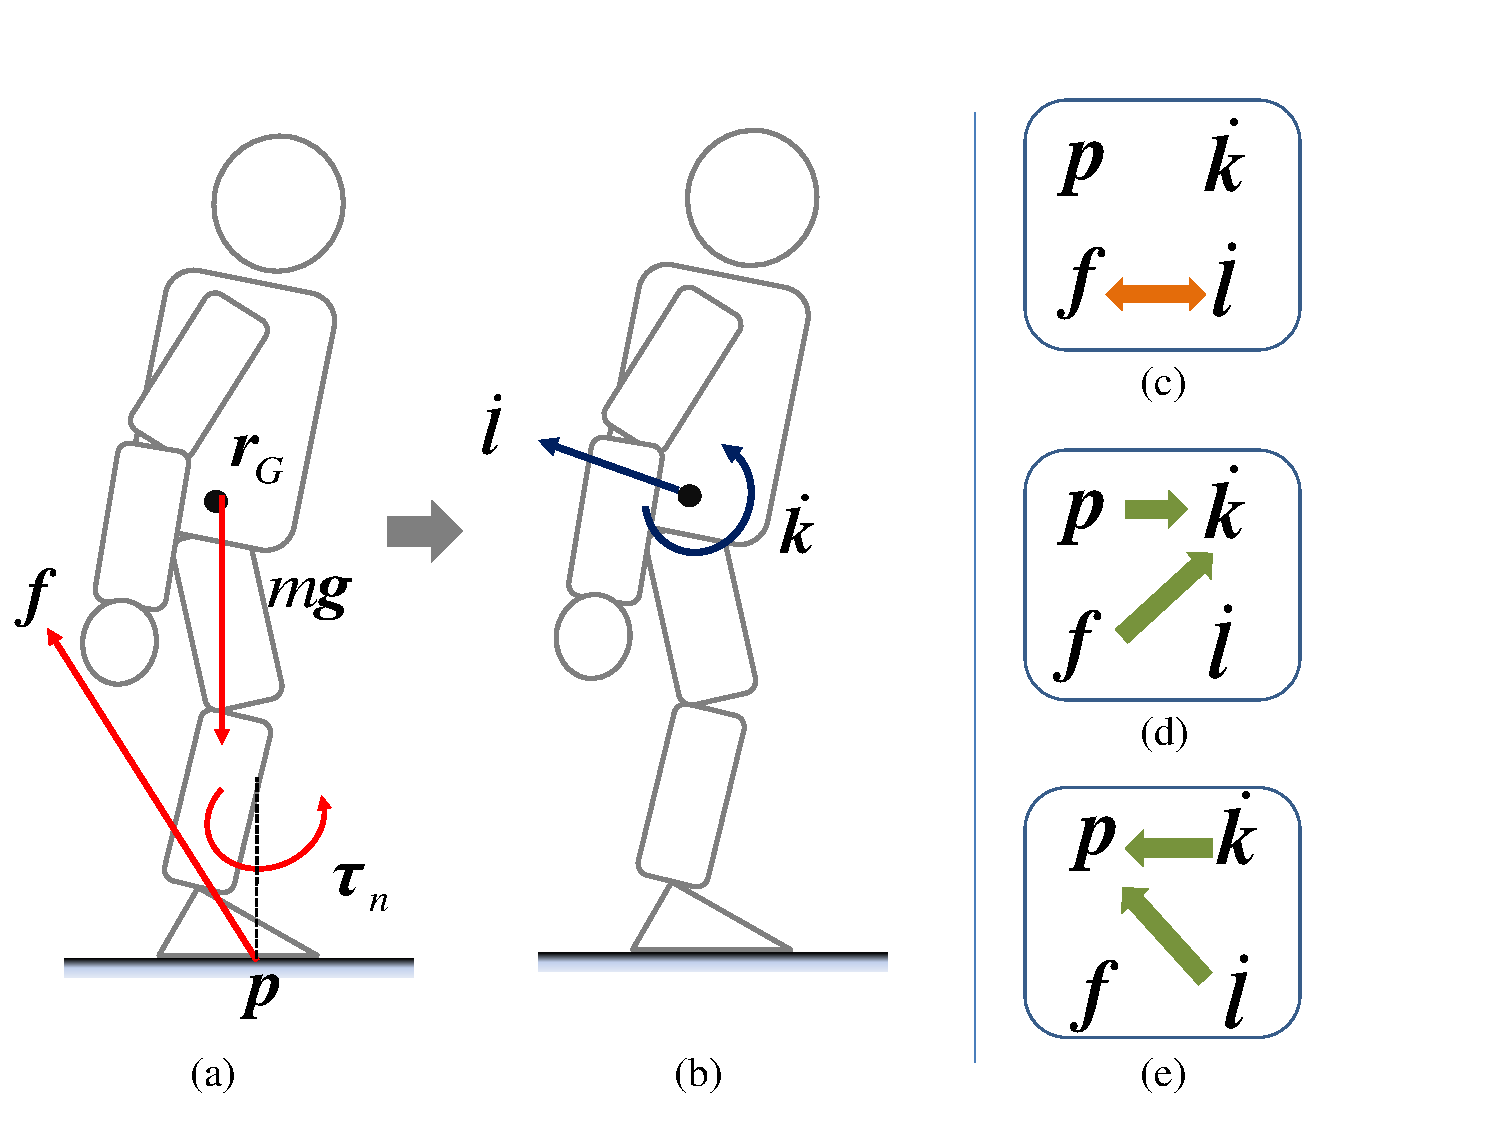
\includegraphics[width=0.5\columnwidth]{Figures/one2one_new_line.pdf}%
\caption{
The external forces and torques in (a) are solely responsible
for the centroidal momentum rate change in (b).
(c): Linear momentum rate change $\vdl$ has a one-to-one
correspondence with the GRF $\vf$.
(d): The centroidal angular momentum rate change $\vdk$
is determined by both $\vf$ and CoP location $\vp$.
(e): Conversely, $\vp$ is determined by both
$\vdl$ and $\vdk$. %
}
\label{fig:one2one}%
\end{center}
\end{figure}

Fig.~\ref{fig:one2one}(a) shows all the external forces that act on a freely
standing humanoid: the GRF $\vf$, the Ground Reaction Moment
$\vtau_n$ normal to the ground, and the weight $m\bg$ of the robot,
where $m$ is the total robot mass and $\bg$ is the acceleration due to gravity. The
sums of external moments and external forces are equivalent to the rates of change of angular and linear momenta, respectively, of the robot, and the mathematical expressions for these relationships are given by (\ref{eq:vdk}) and (\ref{eq:vdl}). Fig.~\ref{fig:one2one}(b) depicts the robot's
 rate of change of angular momentum about the CoM, $\vdk$, and linear momentum, $\vdl$, respectively.
\begin{align}
	\vdk &= (\vp - \vr_G)\times\vf + \vtau_n \label{eq:vdk}\\
	\vdl &= m\vg + \vf \label{eq:vdl}	
\end{align}
In the above equations, $\vr_G$ is the CoM location and $\vp$ is the CoP location.
Together $\vk$ and $\vl$ is a $6\times 1$ vector constitute the spatial centroidal momentum
$\vh_G=[\vk^T~\vl^T]^T$.
In this chapter, we will call it spatial momentum, or simply the momentum of the robot. 
%The aggregate momentum of a humanoid robot may be obtained by summing up all of the angular and linear momenta contributed by the individual link segments.  The centroidal momentum is this aggregate momentum of the robot projected to a reference point instantaneously located at its CoM.
%Note that the spatial centroidal momentunm is computed with respect to a frame which is aligned to the world frame and located at the overall CoM of the robot. Also the frame is instantaneously frozen with respect to the world frame.

Indeed, as noted in \cite{Macchietto09}, the (spatial) momentum
rate change has a one-to-one relationship with the GRF and CoP.
From (\ref{eq:vdl}) and as shown in Fig.~\ref{fig:one2one}(c), $\vdl$ is completely determined by
$\vf$ and vice versa. Furthermore, from (\ref{eq:vdk}) and Fig.~\ref{fig:one2one}(d), a complete
description of $\vdk$ needs both $\vf$ and
$\vp$. Conversely, $\vp$ depends on both $\vdk$ and $\vdl$,  which is shown in Fig.~\ref{fig:one2one}(e).\footnote{The normal torque $\vtau_n$ also affects $\vdk$ in the
transverse plane. Actually $\vf$, $\vp$, and $\vtau_n$ together
constitute the 6 variables that correspond to the 6 variables of the spatial momentum.
Usually $\vtau_n$ is omitted in the discussion for simplicity
because its magnitude is small.}
This last sentence implies that a complete control of $\vp$ is impossible
without controlling both momenta.%Due to this fact, attempts to control CoP by controlling
%only CoM trajectory~\cite{Sugihara02} is fundamentally incomplete.


%%%%%%%%%%%%%%%%%%%%%%%%%%%%%%%%%%%%%%%%%%%%%%%%%%%%%%%%%%%%%%%%%%%%%%%%%%%%%%%
%%%%%%%%%%%%%%%%%%%%%%%%%%%%%%%%%%%%%%%%%%%%%%%%%%%%%%%%%%%%%%%%%%%%%%%%%%%%%%%
\section{Related Work}
%%%%%%%%%%%%%%%%%%%%%%%%%%%%%%%%%%%%%%%%%%%%%%%%%%%%%%%%%%%%%%%%%%%%%%%%%%%%%%%
%%%%%%%%%%%%%%%%%%%%%%%%%%%%%%%%%%%%%%%%%%%%%%%%%%%%%%%%%%%%%%%%%%%%%%%%%%%%%%%


Starting from the early work of~\cite{Vuko69}, researchers have
developed numerous techniques for biped balance control
using various approaches.
Among these are joint control strategies using ankle or hip~\cite{Sano90,Stephens07},
whole body control approaches~\cite{Kagami00,Sugihara02,KKKFHYH03,Choi07,Park05,Stephens10},
methods that find optimal control policies~\cite{Zhou03,Muico09},
and reflex controllers~\cite{Huang05}.
In this section we focus on the research relevant
to momentum-based balance control.

The importance of angular momentum in humanoid walking was reported by Sano and
Furusho as early as 1990~\cite{Sano90}. However, it was much later before its
importance for balance maintenance
of human and humanoid robots started to be seriously explored~\cite{KKKFHYH03,Goswami04,PHH04}.
Sano and Furusho~\cite{Sano90}, and Mitobe et al.~\cite{Mitobe04}
showed that it is possible to generate the desired angular momentum
by controlling the ankle torque.
Kajita et al.~\cite{KKKFHYH03} included angular momentum criteria into the
whole body control framework for balance maintenance.
After expressing desired linear and angular momenta as linear functions of the
generalized velocities, they determined the joint velocities
that achieved both momenta.

Komura et al.~\cite{KLKK05} presented a balance controller that can counteract
rotational perturbations using the Angular Momentum Pendulum Model (AMPM).
This model augments the well known 3D Linear
Inverted Pendulum Model (LIPM)~\cite{KKKYH01} with the additional capability of possessing
centroidal angular momentum.
Naksuk et al.~\cite{Naksuk04} proposed an iterative method
to compute joint trajectories of humanoid robots to satisfy the desired CoM trajectory
and to minimize the centroidal angular momentum.
Other papers that deal with angular momentum for balance
and gait include \cite{Sian03,Ahn06,Ugurlu10,Ye10,Lasa10}.

Abdallah and Goswami~\cite{AG05} defined balance control objectives
in terms of CoM and CoP, and achieved this goal by controlling
the rate of change of linear and angular momenta of a reduced model
humanoid robot. The joint accelerations to generate the target
momentum rate change were resolved using the Moore-Penrose pseudo-inverse.

Hofmann et al.~\cite{Hofmann09} presented a method that
controls CoM by modulating angular momentum under large
external perturbations. It gives higher priority to controlling
linear momentum over angular momentum to enhance the performance
of the balance controller.
%We also give higher priority to attaining the desired linear momentum when both momenta cannot be simultaneously satisfied.

%Our method improves the method in \cite{KKKFHYH03} by providing a step to check for the admissibility of the desired values of linear and angular momenta. Our work is also different from \cite{AG05} and \cite{Macchietto09} in that we define the balance control objectives more intuitively in terms of linear and angular momenta and not in terms of the net CoP.

%Furthermore, our method computes contact forces at each support foot, and therefore can be used both during double-support and single-support and also on non-level, discrete, and non-stationary grounds, whereas \cite{AG05,Macchietto09,Hofmann09} consider only single-support.

Table~\ref{tab:comparison} illustrates how the existing methods treat momentum,
GRF, and CoP in formulating balance and gait strategies.
Robot gait planning methods using reduced models such
as \cite{KKKYH01,Choi07} (Table~\ref{tab:comparison} (a))
compute the necessary CoM trajectory which ensures balance
for a specified desired CoP trajectory.
This is done using reduced models such as the LIPM.
As can be seen from Fig.~\ref{fig:one2one}(e) CoP depends  on both
linear and angular momenta rate changes, so
CoM cannot be uniquely determined solely from CoP.
This was possible in \cite{KKKYH01,Choi07} because the reduced model used in those works
approximated the robot as a point mass, which
can only possess a {\it zero} angular momentum.
%In other words, the resulting CoP-CoM trajectory
%calculated this way induces the unnatural zero rate of change of angular momentum.

In the Resolved Momentum Control approach\cite{KKKFHYH03},
both desired linear and angular momenta are used to determine
joint motion for posture change (Table~\ref{tab:comparison} (b)).
However, the admissibility of the CoP is not considered so the
robot may lose balance if the values of input desired momenta are high.
The methods in Table~\ref{tab:comparison} (c) determine
the desired angular momentum rate change given desired CoP and linear momentum rate change.
In our current method (Table~\ref{tab:comparison} (d)), starting
from the desired linear/angular momenta rate changes, we first determine
admissible foot GRFs and CoPs, and then compute corresponding admissible
momenta rate changes.

\begin{table}[h]
%\begin{minipage}[t]{1.9\columnwidth}
\begin{center}
\caption{The diagrams show how each method
on balance control or gait pattern generation
treats momenta ($\vk,\vl$), GRF ($\vf$),
and CoP ($\vp$). A pair of solid lines determines the target value together.
The dotted line shows the determination process of linear motion and force.
The subscript ``d'' indicates a desired input to the controller
and superscript ``$\ast$'' indicates that the quantity is used to determine control
output such as joint torques.}
\begin{tabular}{c|c|c|c}
\hline
{\scriptsize (a) Kajita } & {\scriptsize (b) Kajita } & {\scriptsize (c) Abdallah and }  & {\scriptsize (d) Lee and }  \\

{\scriptsize et al.~\cite{KKKYH01}, } & {\scriptsize et al.~\cite{KKKFHYH03}} & {\scriptsize Goswami~\cite{AG05},} & {\scriptsize Goswami~\cite{LeeGoswami10},}\\

{\scriptsize Choi et }& &{\scriptsize Macchhietto} & {\scriptsize~\cite{LG12}}\\
{\scriptsize al.~\cite{Choi07}}& &{\scriptsize et al.~\cite{Macchietto09}} & \\
\hline
\hline
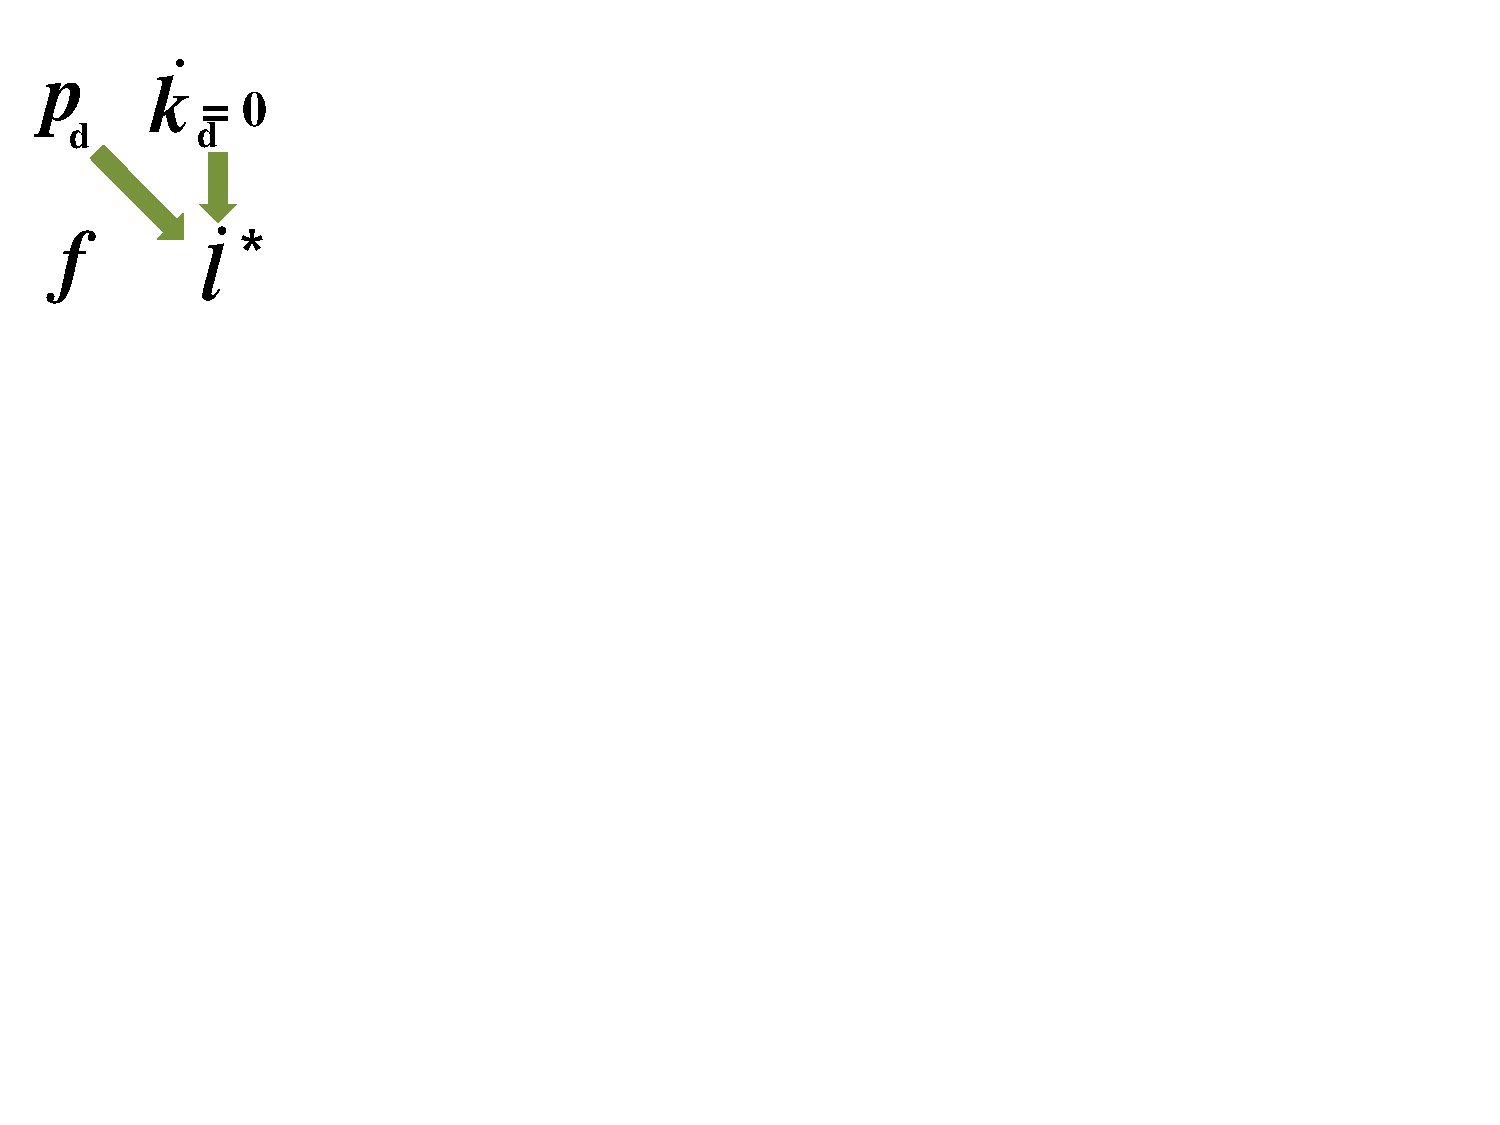
\includegraphics[width=0.13\columnwidth]{Figures/lkpf-diagram-LIPM.pdf}
&
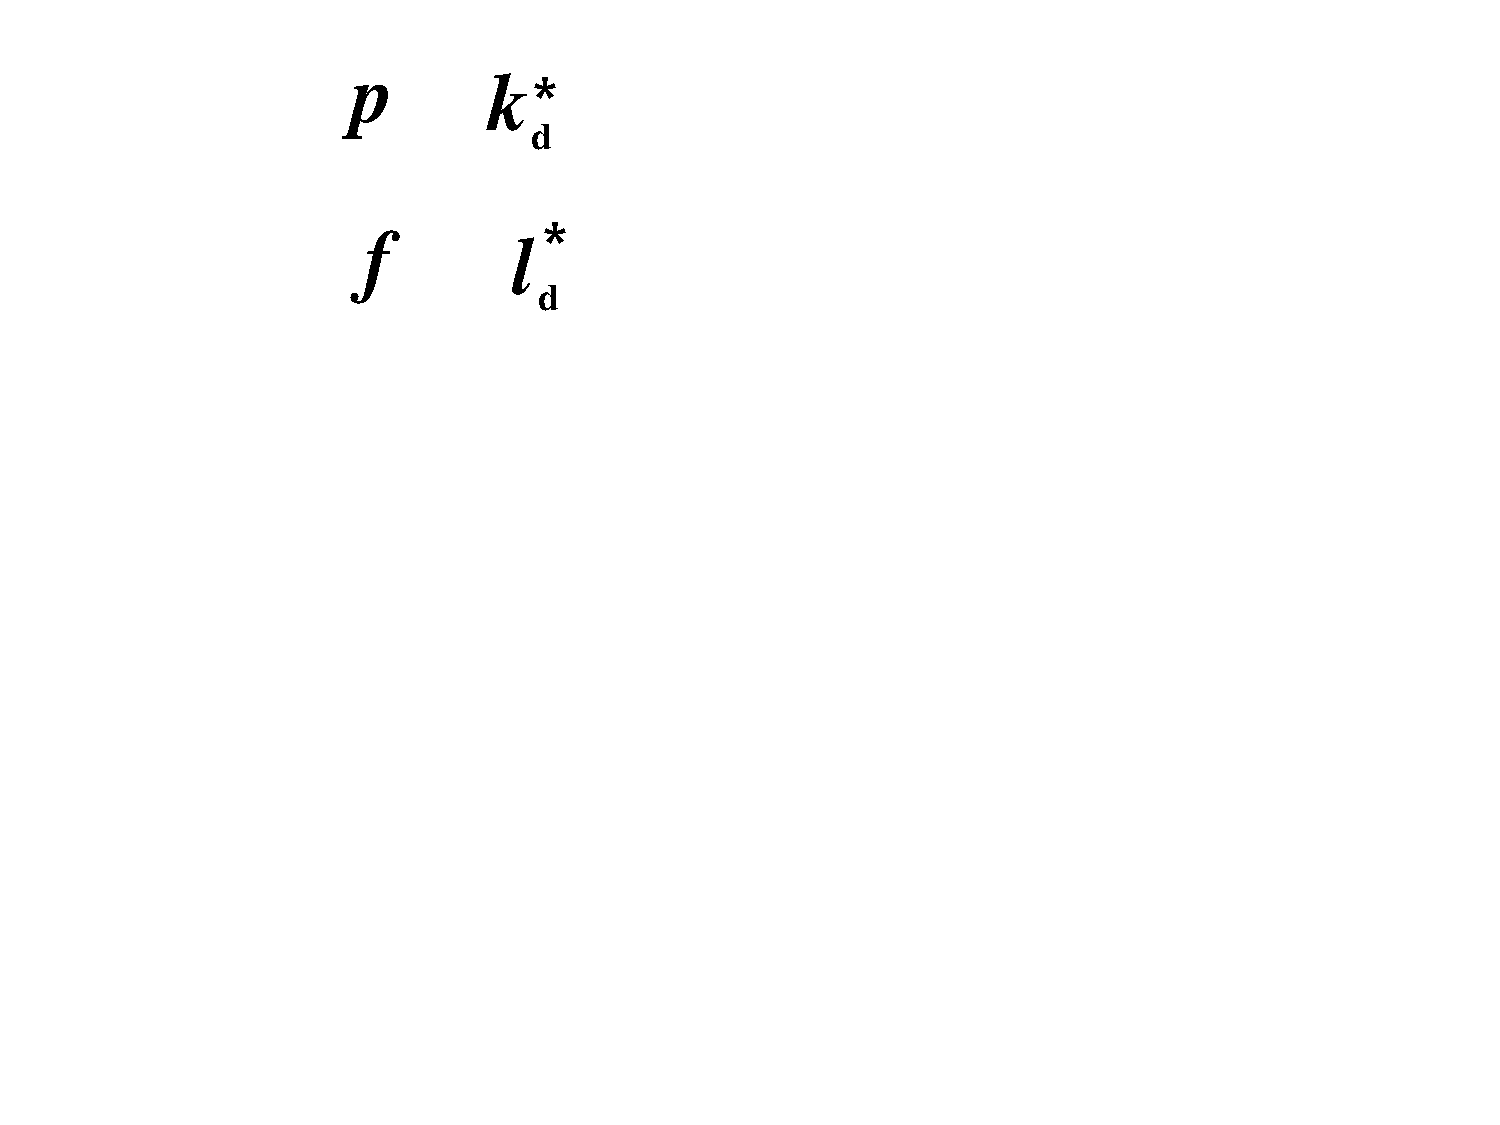
\includegraphics[width=0.13\columnwidth]{Figures/lkpf-diagram-resolvedMomentum.pdf}
&
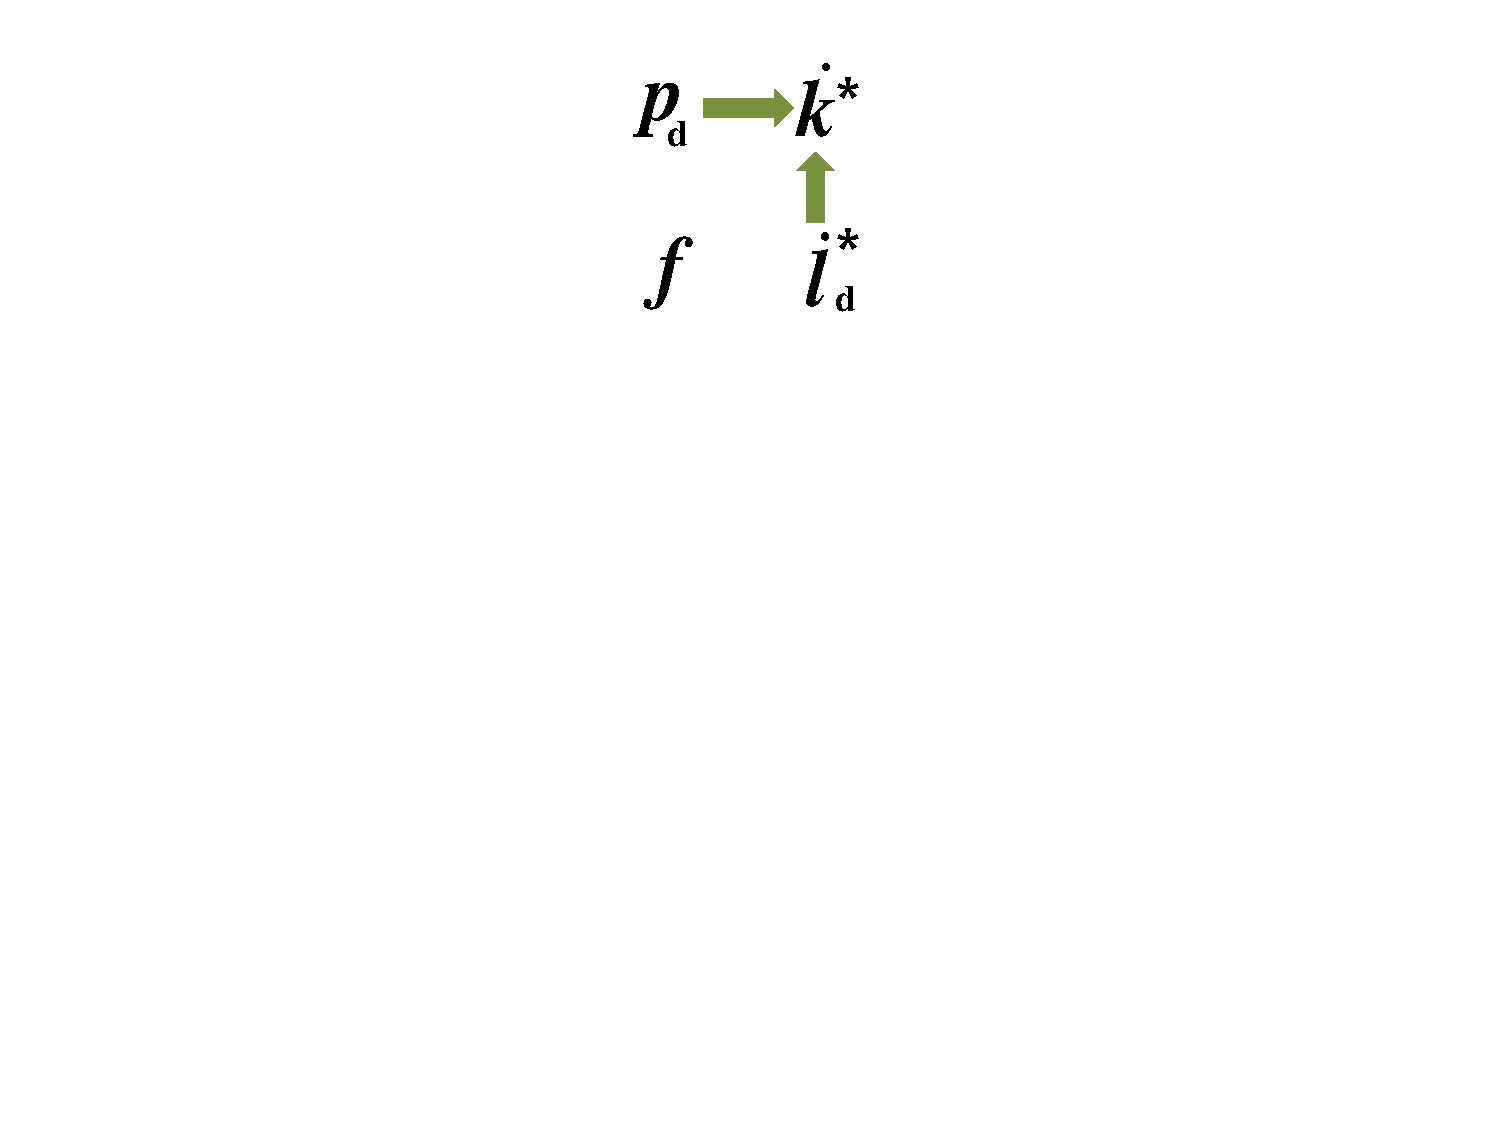
\includegraphics[width=0.13\columnwidth]{Figures/lkpf-diagram-maccietto.pdf}
&
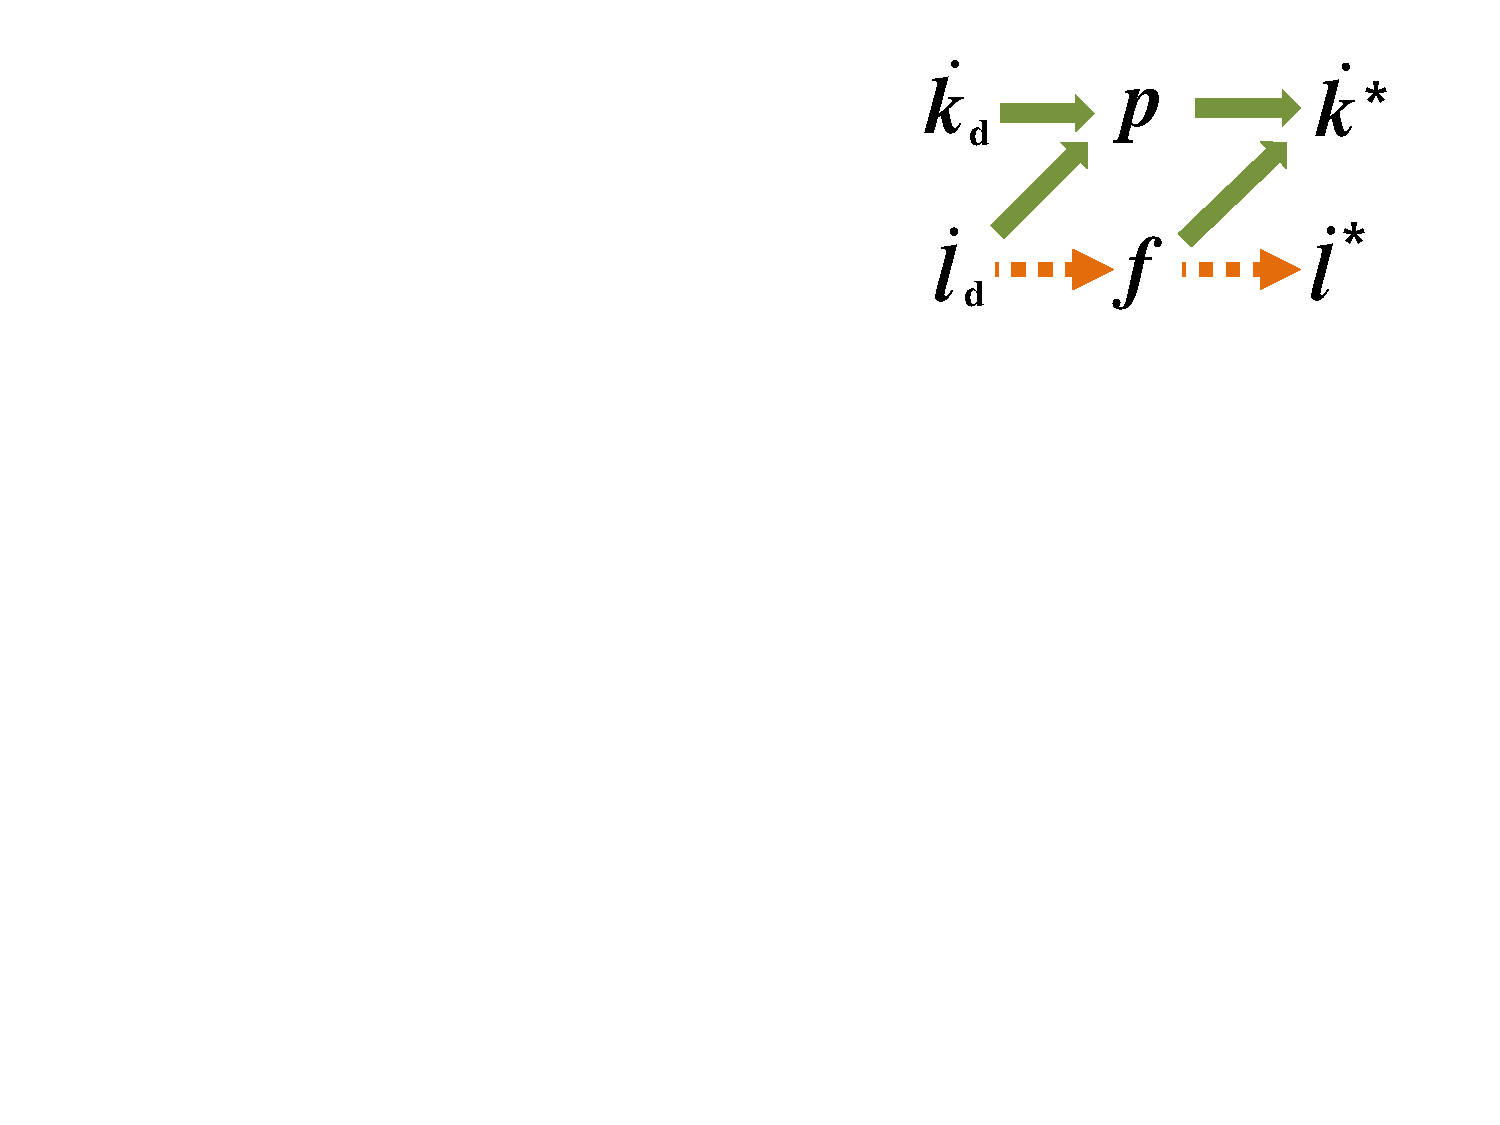
\includegraphics[width=0.23\columnwidth]{Figures/lkpf-diagram-LeeGoswami.pdf} \\
\hline
\end{tabular}
\label{tab:comparison}
\end{center}
%\end{minipage}
\end{table}


%Hyon et al.~\cite{Hyon07} presented a method to resolve foot GRFs and foot CoPs such that they minimize the sum of the squared norm of forces at some points on the boundary of the foot sole while satisfying the desired net GRF and CoP. Their passivity-based controller can remarkably adapt to unknown rough terrain and non-level ground~\cite{Hyon09}. Abe et al.~\cite{Abe07} represented foot GRFs and CoPs in a similar manner to \cite{Hyon07}. This method can minimize each foot GRF if the contact points are well distributed over the foot-ground contact surface. In this paper, we propose a method to distribute the foot GRFs to both feet optimally while minimizing the ankle torques during the double support. Fig.~\ref{fig:FootMinComparison} compares the previous works with our method. 


%In another important work on the control of external forces and torques at each individual foot,
%Fujimoto et al.~\cite{Fujimoto98a,Fujimoto98b,Fujimoto98c} resolved foot GRFs and torques simultaneously using a quadratic programming method.
%In contrast, we  resolve foot GRFs and foot CoPs sequentially, using two least-squares problems, each of which can be solved very quickly. Another notable difference between our work and that of \cite{Fujimoto98a,Fujimoto98b,Fujimoto98c} is that the latter computed external forces and torques from desired accelerations of CoM and trunk orientation whereas we compute them from desired linear and angular momenta rate changes. The advantage of computing desired trunk orientation from external forces and torques is that it can be done more intuitively than computing desired angular momentum, the latter having no direct visible reference. On the other hand, our approach is based on Newton's law, i.e., momentum rate change is completely determined by the external forces and torques. In contrast, the angular acceleration of the trunk cannot be completely determined from the external forces and torques unless the accelerations of other joints are also specified. If these joint accelerations are not incorporated in the force/torque computation, the computed values would be valid only for motions with negligible joint accelerations.

%Sentis et al.~\cite{SPK10} developed a method to precisely control contact CoPs in a more general setting of multicontact interaction between a humanoid robot and the environment using a virtual-linkage model. Park et al.~\cite{Park07} showed that many balancing problems can be framed as the second-order cone programming problem.

%Unlike the above-mentioned approaches which involve distributing the net GRF and net CoP to the supporting feet, Sugihara and Nakamura~\cite{Sugihara03,Sugihara03b} take a different approach that computes the desired acceleration of CoM from the desired foot GRFs and foot CoPs, and then resolves the joint motion to realize the desired acceleration of CoM. This method has the merit of offering an easy manipulation of contact state between individual foot and the ground but, as mentioned in \cite{Sugihara03,Sugihara03b} by the authors themselves, is not guaranteed to realize the desired foot CoP and GRF during double support.

Ugurlu and Kawamura have studied bipedal walking that
specifically controls the centroidal angular momentum~\cite{UK10}.
Relatively recently we have seen a comprehensive
study of angular momentum during human gait~\cite{HP08}.


%%%%%%%%%%%%%%%%%%%%%%%%%%%%%%%%%%%%%%%%%%%%%%%%%%%%%%%%%%%%%%%%%%%%%%%%%%%%%%%
\subsection{Comparison with ZMP-based control}
%%%%%%%%%%%%%%%%%%%%%%%%%%%%%%%%%%%%%%%%%%%%%%%%%%%%%%%%%%%%%%%%%%%%%%%%%%%%%%%

Earlier approaches to humanoid walking control involved planning joint motions such that a 
given reference ZMP trajectory was achieved \cite{nishiwaki2001online}.
The motion planning was performed offline, and the resulting joint trajectories were then tracked 
using PID or similar controllers.
The problem with this approach is that it is very brittle;  it is not robust to balance disturbances
because the joint controllers have no knowledge about the relation between CoM and ZMP, which is 
fundamental to balance.
This basic approach of playing back pre-computed joint trajectories has also been used extensively
in hobby robots such as the ones used in the Robo One competitions \cite{roboone}.  
The result is predictable;  the robots fall over very easily.
Despite its problems, a key advantage of this approach is that it does not require use of an
\textit{Inertial Measurement Unit} (IMU) to estimate key aspects of robot state, such as CoM position
and velocity.  
This has become less of an advantage in recent years as the price of accurate 
IMU units has dropped dramatically.
Robot state estimation will be discussed in more detail, subsequently.

An early variation of the pre-computed trajectory approach involved computing the joint motions 
online, but still with the goal of following a reference ZMP trajectory \cite{nishiwaki2002online, 
kagami2002fast, sugihar2002real}.  
While this is an improvement in that it doesn't blindly follow
joint trajectories, it still has a fundamental problem.
As will be explained in more detail in the next section, the ZMP is not the desired quantity to be
controlled. 
The actual quantity to be controlled is momentum, or, related to this, the position and velocity of the 
robot's CoM.
The ZMP is, effectively, a control input;  manipulation of the ZMP has the effect of accelerating the CoM.
Thus, while using a reference ZMP trajectory as a feed-forward term may be useful,
tracking a reference ZMP trajectory exclusively, without feedback terms based on the true
quantities to be controlled (CoM state), results in an unstable system.



%%%%%%%%%%%%%%%%%%%%%%%%%%%%%%%%%%%%%%%%%%%%%%%%%%%%%%%%%%%%%%%%%%%%%%%%%%%%%%%
\section{Computing Momentum of a Humanoid Robot}
%%%%%%%%%%%%%%%%%%%%%%%%%%%%%%%%%%%%%%%%%%%%%%%%%%%%%%%%%%%%%%%%%%%%%%%%%%%%%%%


%%%%%%%%%%%%%%%%%%%%%%%%%%%%%%%%%%%%%%%%%%%%%%%%%%%%%%%%%%%%%%%%%%%%%%%%%%%%%%%
\subsection{Humanoid robot model}
\label{sn}
%%%%%%%%%%%%%%%%%%%%%%%%%%%%%%%%%%%%%%%%%%%%%%%%%%%%%%%%%%%%%%%%%%%%%%%%%%%%%%%

A humanoid can be modeled as a set of $N+1$ links interconnected by $N$ joints,
of up to six degrees of freedom each, forming a tree-structure topology.
The motion of the links are referenced to a fixed base (inertial frame)
which is labeled 0 while the links are labeled from 1 through $N$.
Numbering of the links may be done in any manner such that link $i$'s
predecessor toward the root (link 0), indicated by $p(i)$, is always
less than $i$.  Joints in the tree are numbered such that joint $i$
connects link $i$ to link $p(i)$.  A coordinate frame is attached to each
link to provide a reference for quantities associated with the link.

%The relationship between connected links in the tree structure is described using the general joint model of Roberson and Schwertassek~\cite{RoSc88}.
An $n_i \times 1$ vector $\dot{\bq}_i$ relates the velocity of link $i$
to the velocity of its predecessor, link $p(i)$, where $n_i$ is the number
of degrees of freedom at the joint connecting the two links.  The free
modes of the joint are represented by the $6 \times n_i$ matrix
$\vPhi_i$, such that the spatial velocity of link $i$ is given as
follows:
%
%
\begin{equation}
\label{eq:spatialvelocity}
\bv_i =        \left[ \begin{array}{c} \vomega_i \\ \vv_i \end{array} \right] =
\XM{i}{p(i)} \, \bv_{p(i)} + \vPhi_i \, \vqd_i \; ,
\end{equation}
%
where $\vomega_i$ and $\vv_i$ are the angular and linear velocities
of link $i$, respectively, as referenced to the
link coordinate frame.
We will use spatial notation \cite{FeOr08,Featherstone87} for describing rigid-body velocity, acceleration, inertia, etc., using 6D vectors and tensors.
$\XM{i}{p(i)}$ is a $6 \times 6$ spatial
transform which transforms spatial motion vectors from $p(i)$ to $i$
coordinates.  The matrix $\vPhi_i$ depends on the type of joint
\cite{FeOr08}. % It has full column rank, as does the orthogonal matrix $\vPhi_i^c$ representing the constrained modes of the joint, such that $\left[ \vPhi_i \; \; \vPhi_i^c \right]$ is a basis of $\mathbb{R}^6$ and is invertible.
For instance, $\vPhi_i = \left[ 0 \, 0 \, 1 \, 0 \, 0 \, 0 \right]^T$ for a
revolute joint with the rotation axis being aligned with the Z-axis. 

In order to model a humanoid when in flight, one of the links is
modeled as a floating base (typically the torso) and numbered as link 1.
A fictitious six degree-of-freedom (DoF) joint is inserted between the
floating base and fixed base.  In this case, $\vPhi_1 = \bone_{6 \times 6}$
where $\bone_{6 \times 6}$ is the identity matrix.  The total number of degrees of freedom in the
humanoid is $n$ where $n= \sum n_i$.  Note that $n$ includes the
six degrees of freedom for the floating base.

The spatial transform $\XM{i}{p(i)}$ may be composed from the position
vector $\Pos{p(i)}{i}$ from the origin of coordinate frame $p(i)$ to
the origin of $i$, and
the $3 \times 3$ rotation matrix $\Rot{i}{p(i)}$ which transforms
3D vectors from coordinate frame $p(i)$ to $i$:
%
\begin{equation}
\label{eq:ST}
\XM{i}{p(i)}
= \BM \Rot{i}{p(i)} & \bzero \\
              \Rot{i}{p(i)} \,\vS(\Pos{p(i)}{i})^T & \Rot{i}{p(i)} \EM \, .
\end{equation}
%
The quantity $\vS(\vp)$ is the skew-symmetric matrix that satisfies
$\vS(\vp)\,\vomega = \vp \times \vomega$ for any 3D vector $\vomega$.

It is possible to combine the equations for the velocity or momentum
for all the links into a global set of equations.  To do
so, composite vectors and matrices are defined. %, and this was the starting point of the spatial operator algebra developed by Rodriguez et al.~\cite{RoJa91}.  
Global notation is useful
in developing a system Jacobian which leads to an
expression for the Centroidal Momentum Matrix.

Gathering all of the link velocities and joint velocities together, the system Jacobian $\bJ$ can be defined to give the relationship between the two:
%
\begin{equation}
\label{eq:v}
\bv = \bJ \, \bqd \; ,\\
\end{equation}
%
where %
\begin{equation}
\bv = \left[ \bv_1^T, \, \bv_2^T, \cdots \bv_i^T, \cdots \bv_N^T \right]^T \, .
\end{equation}

The elements of the system Jacobian are just the Jacobians for each of the links:
%
\begin{equation}
\bJ = \left[ \vJ_1^T, \, \vJ_2^T, \cdots \vJ_i^T, \cdots \vJ_N^T \right]^T \, .
\end{equation}




%%%%%%%%%%%%%%%%%%%%%%%%%%%%%%%%%%%%%%%%%%%%%%%%%%%%%%%%%%%%%%%%%%%%%%%%%%%%%%%
\subsection{Multibody system momenta}
%%%%%%%%%%%%%%%%%%%%%%%%%%%%%%%%%%%%%%%%%%%%%%%%%%%%%%%%%%%%%%%%%%%%%%%%%%%%%%%

\begin{figure}[t]
\begin{center}
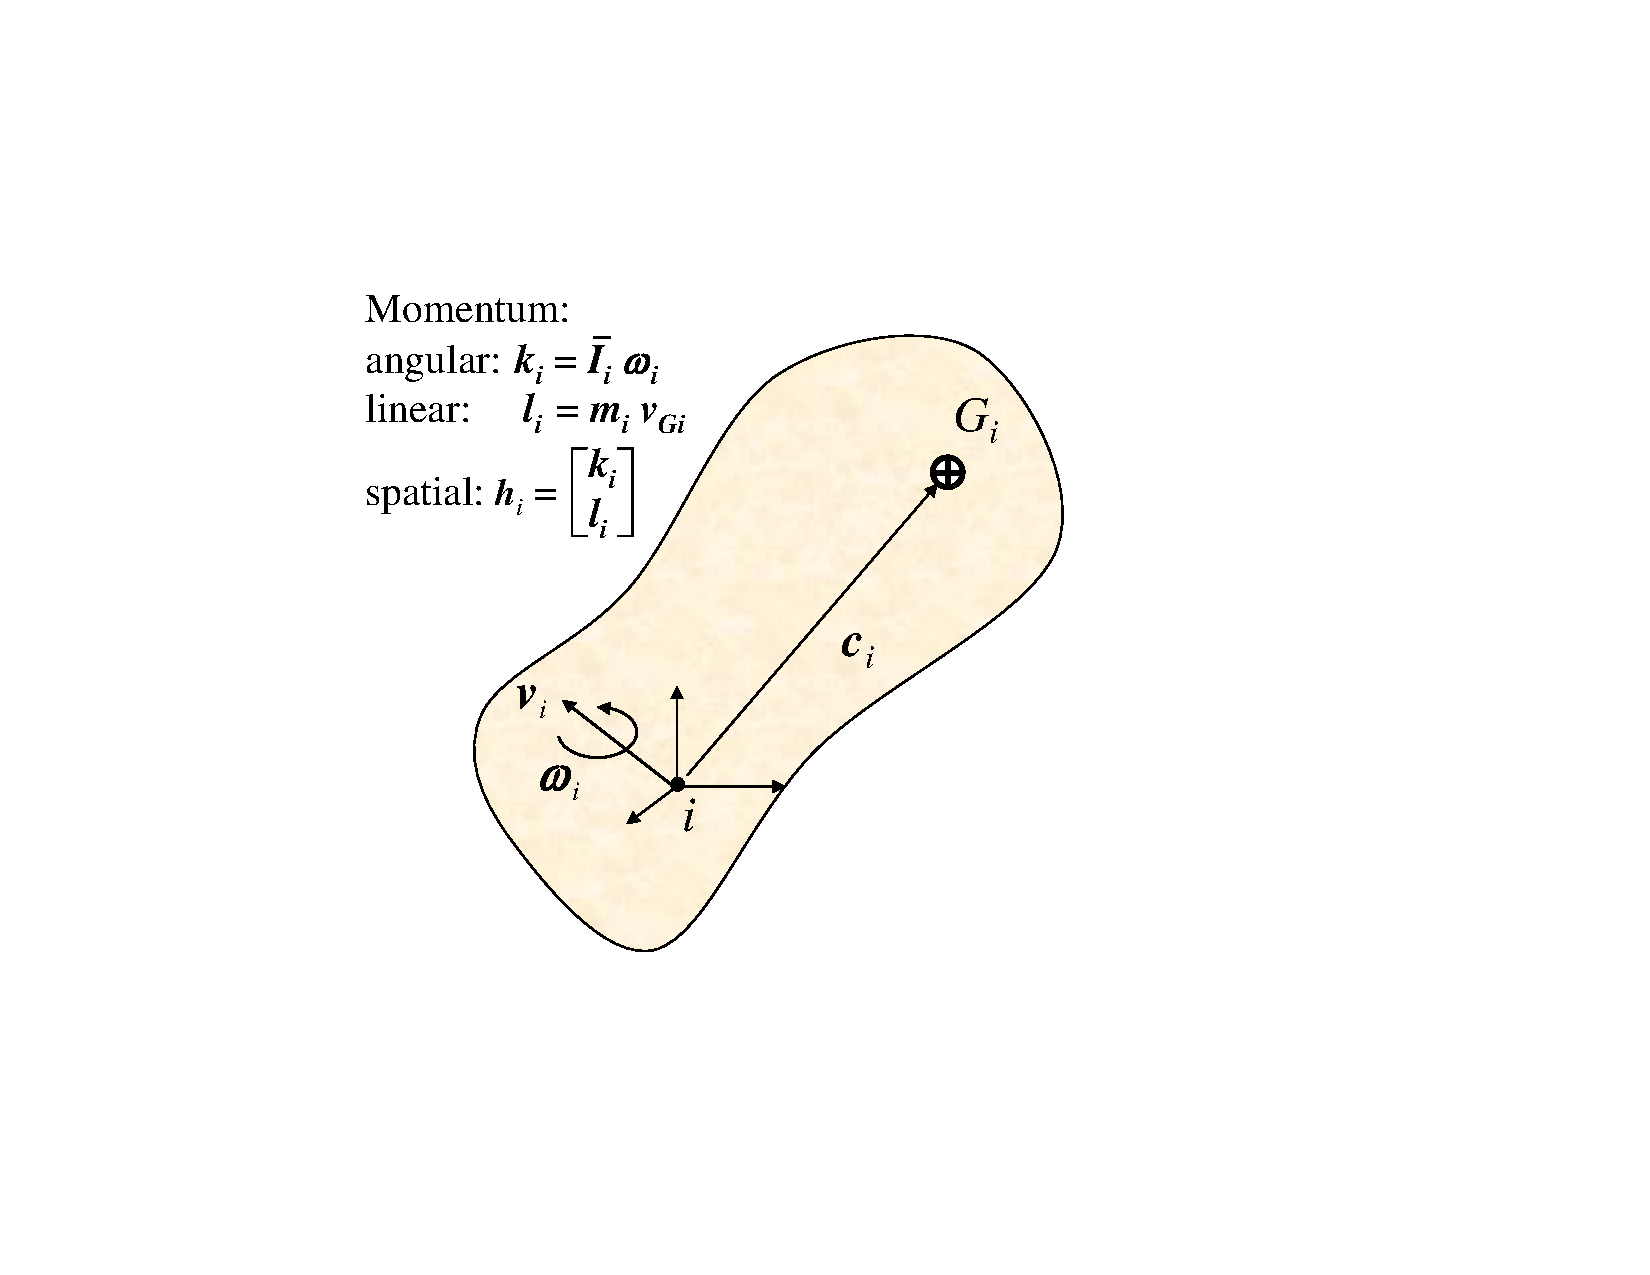
\includegraphics[width=2.0in]{Figures/fig1.pdf}
\end{center}
\caption{Schematic depiction of a single rigid body:
spatial momentum contains the angular and linear momenta.} \label{fig1}
\end{figure}


The spatial momentum of each link may be computed from the spatial velocity as follows
(see Fig.~\ref{fig1}):
%
\begin{equation}
\bh_i = \left[ \begin{array}{c} \vk_i \\ \vl_i \end{array} \right] = \vI_i \, \bv_i \, ,
\end{equation}
%
where $\vk_i$ is the angular momentum, $\vl_i$ is the linear
momentum, and $\vI_i$ is the spatial inertia for link $i$. The
spatial inertia may be composed from the mass $m_i$, position vector $\vc_i$
to the center of mass (CoM)  of link $i$, and $3 \times 3$ rotational
inertia $\vIb_i$, all relative to coordinate frame $i$:

\begin{equation}
\label{eq:spatialinertia}
\vI_i =
\BM
  \vIbar_i & m_i \, \vS(\vc_i) \\ m_i \, \vS(\vc_i)^T & m_i \, \bone
\EM ,
\end{equation}
%
where
%
\begin{equation}
\vIbar_i = \vIbar^{cm}_i \!\! + m_i \, \vS(\vc_i) \, \vS(\vc_i)^T \, ,
\end{equation}
%
and $\vIbar^{cm}_i$ is the rotational inertia about the CoM.
Recall that if the origin of coordinate frame $i$ is chosen
at the CoM, the off-diagonal blocks $m_i \, \vS(\vc_i)$
reduce to zero. If, in addition, the axes of coordinate frame $i$
are oriented along the principal axes of inertia, $\vIbar_i$ becomes a
$3\times 3$ diagonal matrix and $\vI_i$ a $6\times 6$ diagonal matrix.


The momenta of all the links in the system may be determined as the
product of the system velocity vector $\bv$ and the system inertia
$\bI$; gathering all:
%
\begin{equation}
\label{eq:h}
\bh = \bI \, \bv \; ,
\end{equation}
%
where $\bh$ is the $6N\times 1$ system momentum vector $\bh = \left[ \bh_1^T, \, \bh_2^T, \cdots \bh_i^T, \cdots \bh_N^T \right]^T,$
and the $6N \times 6N$ system inertia matrix is defined as
$\bI = \diag \left[ \vI_1, \, \vI_2, \cdots \vI_i, \cdots \vI_N \right] \, .$
%

%In conclusion to this section, let us note that spatial notation results in compact equations whose vectors and matrices contain both angular and linear parts. Further, the use of global notation illuminates the underlying structure of centroidal dynamics as we will see in the next section.


%%%%%%%%%%%%%%%%%%%%%%%%%%%%%%%%%%%%%%%%%%%%%%%%%%%%%%%%%%%%%%%%%%%%%%%%%%%%%%%
\subsection{Centroidal momentum}
%%%%%%%%%%%%%%%%%%%%%%%%%%%%%%%%%%%%%%%%%%%%%%%%%%%%%%%%%%%%%%%%%%%%%%%%%%%%%%%

The aggregate momentum of a humanoid may be obtained by summing up all of the angular and linear momenta contributed by the individual link segments. 
As defined, the spatial momentum of each link $\bh_i$ is most
naturally expressed in its own coordinate system.  As a measure of
dynamic stability or for control, it is useful to combine the
momenta for the links by projecting the momenta to a common
coordinate frame.  A convenient frame is one set at the
instantaneous CoM or the centroid of the system
$G$, and whose coordinate axes are parallel to those of the inertial coordinate frame 0.
The $6\times 1$ centroidal momentum vector $\bh_G$, which
consists of the linear and centroidal angular momenta of the robot, is the aggregate momentum with respect to the above-mentioned centroidal frame.
Noting that the spatial momentum may be projected as any other
force-type vector~\cite{FeOr08}, the following equation may be used to calculate
the spatial momentum at the centroid of the system (see Fig.~\ref{biped}):
%
\begin{equation}\label{hgt}
\bh_G = \sum_{i=1}^N  \XM{i}{G}^T \, \bh_i = \bX_G^T \, \bh \; ,\\%\sum_{i=1}^N \XM{i}{G}^T \, \bA_i \, \bqd \; .\\
\end{equation}
%
%
where $\bX_G$ is defined as the projection matrix, for motion vectors,
from centroidal coordinates to link coordinates and is given as follows:
%
\begin{equation}
\bX_G = \left[ \begin{array}{c} \XM{1}{G}^T, \, \XM{2}{G}^T, \,
\cdots \XM{i}{G}^T, \, \cdots \XM{N}{G}^T \end{array} \right]^T \; .
\end{equation}
%
%------------------------------------------------------------------------

\begin{figure}[h]
\begin{center}
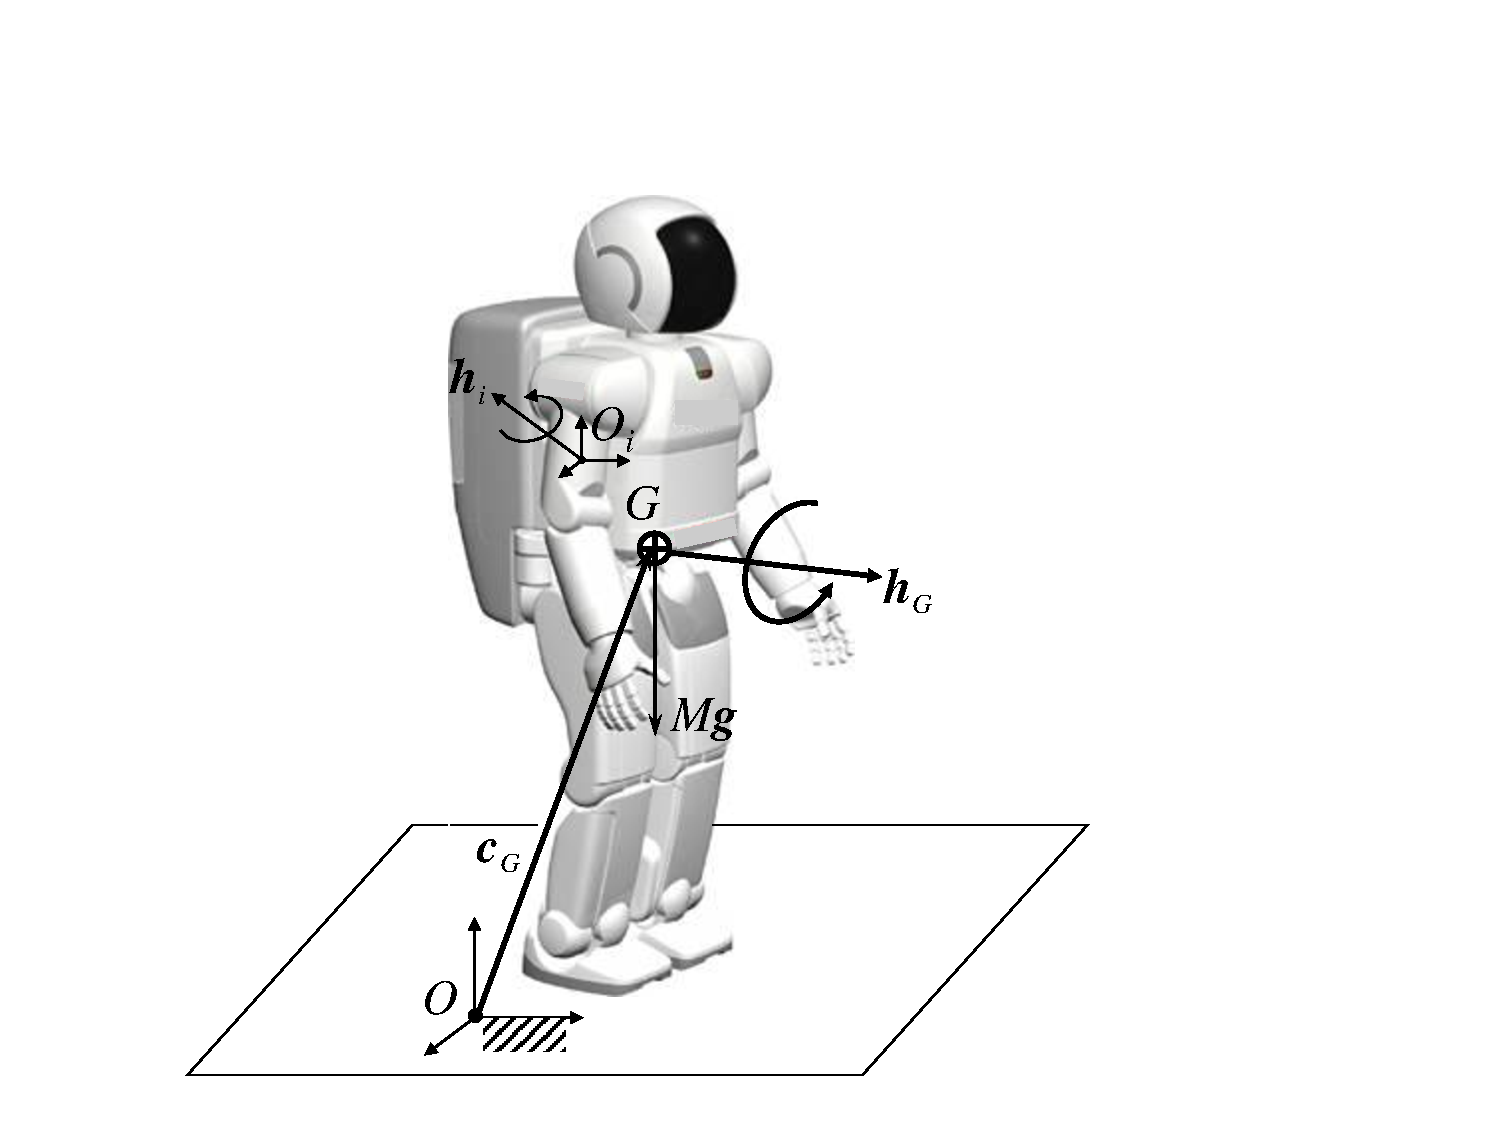
\includegraphics[width=3.0in]{Figures/bop1.pdf}
\end{center}
\caption{Humanoid robot showing link and centroidal momentum vectors. The inertial frame
is located at $O$ and the position vector to the robot CoM, $G$, is given by $\bc_G$. The reference frame of
link $i$ is located at $O_i$. The centroidal momentum
$\bh_G$ can be obtained from either Eq.~\ref{eq:centroidalmomentum} or Eq.~\ref{hgt}.} \label{biped}
\end{figure}


The centroidal momentum vector $\bh_G$ is related to its $n\times 1$ joint velocity vector $\dot\bq$ as:
\begin{equation}
\label{eq:centroidalmomentum} \bh_G = \bA_G(\bq) \, \dot\bq \, .
\end{equation}
%
The $6\times n$ matrix $\bA_G$ is called the
\emph{Centroidal Momentum Matrix} and $\bA_G$ contains contributions
both from the inter-segmental joint variables of the robot as well as
from the fictitious joint connecting the floating base of the humanoid to the inertial frame
(detailed in Section~\ref{sn}). Note that $\bA_G$
is identical to the large matrix in the RHS of Eq.~1 of \cite{KKKFHYH03}, with only
the linear and angular parts interchanged.

%The literature contains relatively few references to matrices that map joint rates into aggregate momenta of a multibody dynamic system. In \cite{FP03} the ``linear momentum Jacobian" is obtained as an intermediate step towards computing what the authors refer to as a force Jacobian. This formulation is used for animating articulated figures and does not contain angular momentum. In \cite{MO03} the ``angular momentum Jacobian" matrix is used to control the flight phase of a hopping robot. Finally, for resolved momentum control of humanoid robots, use has been made of ``matrices which indicate how the joint speeds affect the linear momentum and angular momentum"~\cite{KKKFHYH03}. Although they have been called ``inertia matrices" in this work, these matrices are identical to the ``momentum Jacobian" matrices mentioned before.

%Is $\bA_G$ an inertia matrix or a Jacobian matrix? In the following development, we will show that $\bA_G$ can be represented as the product of a spatial transformation matrix, an inertia matrix, and a Jacobian matrix.  In Section \ref{TD}, we show its relationship to other important quantities including the joint-space inertia matrix.

%%%%%%%%%%%%%%%%%%%%%%%%%%%%%%%%%%%%%%%%%%%%%%%%%%%%%%%%%%%%%%%%%%%%%%%%%%%%%%%
%\subsection{Formulation of Centroidal Momentum Matrix}
%%%%%%%%%%%%%%%%%%%%%%%%%%%%%%%%%%%%%%%%%%%%%%%%%%%%%%%%%%%%%%%%%%%%%%%%%%%%%%%

As shown in Eq.~\ref{eq:centroidalmomentum}, the CMM
gives the relationship between the joint rates and centroidal momentum.
In order to find the relationship between this matrix and the link
inertias and Jacobians, the concept of the \emph{system momentum
matrix} $\bA$ is first presented. The system momentum matrix
$\bA$ expresses the relationship between the
system momentum vector and the joint rates:
$\bh = \bA \, \bqd$~.

Substituting the expression for the system velocity
in Eq.~\ref{eq:v} into Eq.~\ref{eq:h},
%gives:
%
%\begin{equation}\label{eq:hij}
%\bh = \bI \; \bJ \; \bqd \; .\\
%\end{equation}
%
%From this,
and using the definition of the system momentum matrix, we can write:
%
\begin{equation}\label{eq:a}
\bA = \bI \; \bJ \; .\\
\end{equation}
%
The system momentum matrix is just the product of the system inertia
matrix and the system Jacobian. It includes the momentum matrix for
each link and is of size $6N \times n$:
%
\begin{equation}\label{eq:A}
\bA = \left[ \begin{array}{c} \bA_1^T, \, \bA_2^T, \, \cdots \bA_i^T, \, \cdots \bA_N^T \end{array} \right]^T \; ,
\end{equation}
%
with
%
%\begin{equation}
$\bA_i = \bI_i \; \bJ_i$ .
%\end{equation}
%


%The system momentum vector, as defined above, includes the
%individual spatial momenta for the links:
%
%\begin{equation}
%\bh = \left[ \bh_1^T, \, \bh_2^T, \cdots \bh_i^T, \cdots \bh_N^T
%\right]^T \; .
%\end{equation}%
%Also,



%The above equation is analogous to Eq.\ref{hg2}. In $\XM{i}{G}^T$ the rotational part is
%not well-defined, because CoM doesn't define a coordinate frame but only a point.

%The centroidal momentum may be expressed as a function of the system momentum:
%
%\begin{equation}\label{hgt}
%\bh_G = \bX_G^T \, \bh  \, ,
%\end{equation}
%
%where $\bX_G$ is defined as the projection matrix, for motion vectors,
%from centroidal coordinates to link coordinates and is given as follows:
%
%\begin{equation}
%\bX_G = \left[ \begin{array}{c} \XM{1}{G}^T, \, \XM{2}{G}^T, \,
%\cdots \XM{i}{G}^T, \, \cdots \XM{N}{G}^T \end{array} \right]^T \; .
%\end{equation}
%
%------------------------------------------------------------------------
%By defining the projection matrix from link coordinates to CoM
%coordinates as follows:
%
%\begin{equation}
%\bX_G = \left[ \begin{array}{c} \XM{1}{G}^T, \, \XM{2}{G}^T, \,
%\cdots \XM{i}{G}^T, \, \cdots \XM{N}{G}^T \end{array} \right]^T \; ,
%\end{equation}
%
%------------------------------------------------------------------------
%
The centroidal momentum may also be expressed as a function of the
system momentum matrix $\bA$:
%
\begin{equation}\label{hgt2}
\bh_G = \bX_G^T \, \bA \, \bqd \; .
\end{equation}
%
Noting Eqs.~\ref{eq:centroidalmomentum} and \ref{hgt2}, and
using the expression for $\bA$ in Eq.~\ref{eq:a}, the CMM, $\bA_G$, may then be defined as:
%
\begin{equation}\label{eq:Ag}
\bA_G = \bX_G^T \, \bA = \bX_G^T \, \bI  \, \bJ \; ,
\end{equation}
%
%so that it gives the relationship between the centroidal momentum
%and the joint rates, Eq.~\ref{eq:centroidalmomentum}.
%
%Substitution of Eq.~\ref{eq:a} into Eq.~\ref{eq:Ag} gives
%
%\begin{equation}
%\bA_G = \bX_G^T \, \bI  \, \bJ \; ,
%\end{equation}
%
which
%Equation~\ref{eq:Ag}
shows the relationship between $\bA_G$ and the system inertia and Jacobian.
Furthermore, time differentiation of Eq.~\ref{eq:centroidalmomentum} results in the following relation
which forms the basis of our momentum-based balance controller presented later in this chapter:
\begin{equation}
\label{eq:hGdot}
\vdh_G = \bA_G \, \vddq + \dot\bA_G \, \bqd \; .
\end{equation}
%
Finally, since $\Bf=\vdh_G$ (Newton's equations of motion) where $\Bf$ is the net external force/moment on the system, then it may be noted that $\bA_G$ gives the relationship between the net external force/moment and the joint accelerations.




%%%%%%%%%%%%%%%%%%%%%%%%%%%%%%%%%%%%%%%%%%%%%%%%%%%%%%%%%%%%%%%%%%%%%%%%%%%%%%%
%\subsection{A word on ground reaction force}
%%%%%%%%%%%%%%%%%%%%%%%%%%%%%%%%%%%%%%%%%%%%%%%%%%%%%%%%%%%%%%%%%%%%%%%%%%%%%%%




%%%%%%%%%%%%%%%%%%%%%%%%%%%%%%%%%%%%%%%%%%%%%%%%%%%%%%%%%%%%%%%%%%%%%%%%%%%%%%%
%\section{Control Problem Statement}
%\label{sec:problemstatement}
\section{Approaches to Momentum-Based Balance Control}
\label{sec:approaches}
%%%%%%%%%%%%%%%%%%%%%%%%%%%%%%%%%%%%%%%%%%%%%%%%%%%%%%%%%%%%%%%%%%%%%%%%%%%%%%%

%In this section, we introduce the types of tasks that we would like a humanoid robot to perform, and define what it means to maintain balance while performing these tasks.  We also discuss the implied requirements for a balance controller.

% First, introduce tasks to be accomplished, and how they should be specified




\subsection{Centroidal-Moment Point-Based Balance Control }

Not all tasks for humanoid forms necessarily require balance as an end goal. 
For example, a football player trying to score a touchdown, or a baseball player trying to catch a fly ball,
does not care if he is upright at the end, as long as the goal is achieved.
For the subsequent discussion, however, we assume that balance control is included as an end goal in a task specification.
% Note that it is not necessarily an intermediate goal.  Often, in single support, full balance control is not possible.
% However, the intent is to ``catch'' things so that in the subsequent double support phase, full balance control is
% achieved.

This naturally leads us to the need for a precise definition of balance control.
Consider a horizontal plane that intersects the CoM, and that is perpendicular to the gravity vector.
We define balance control as the ability to accelerate the CoM in any direction in this 
horizontal plane.
[This isn't complete enough.  See better problem definition in the introduction.]

% Make this a formal definition?  Show diagram of plane, or is this obvious?

% Give example.

In order to understand this problem in more detail, it is useful to develop a basic model that incorporates
all the quantities of interest.
[The following may be, to some extent, redundant with what has already been presented.
Talk to Ambarish about how to collapse].



Balance control, as defined above, requires the ability to adjust the humanoid biped’s linear and angular momentum.  
Due to conservation of momentum laws, such adjustment can only be achieved through force interaction with the environment.  
For a biped, this force interaction is comprised of gravity and the ground reaction force, the net force exerted by the ground against the biped.  
The following analysis of physical constraints and requirements for balancing leads to a simple, comprehensive model of balance control that specifies 
coordination of control actions that adjust the ground reaction force, and therefore, the momentum of the biped.
Similar models have been used previously in a number of gait planning algorithms 
\cite{kajita2001real, yokoi2001honda, sugihara2002real, nishiwaki2002online}.
These models utilize analysis of inverted pendulum dynamics \cite{formal2006inverted}.
A key difference in the model presented here is its ability to 
purposely sacrifice angular momentum control goals in order to achieve linear control goals when both cannot be met.  

The model makes use of a number of physical points that summarize the system’s balance state.  
These points are the center of mass (CoM), the zero-moment point (ZMP) \cite{vukobratovic69},
and the centroidal-moment point (CMP) \cite{popovic2005ground}.  
The ZMP is a point on the ground that represents the combined force interaction of all ground contact points.  
The CMP is the point on the ground from which the ground reaction force would have to emanate if it were to produce no torque about the CoM. 
These points will be defined more formally in the following discussion.

% Support base
A biped’s \textit{support base} is defined as the smallest convex polygon that includes all points where the feet are in contact with the ground.  
When in single support, that is, where one foot, the stance foot, is on the ground and the other is stepping, the support base is the outline of the part of 
the stance foot that is in contact with the ground.  
When in double support, that is, where both feet are on the ground, the base of support is the smallest convex polygon that includes all points where the two feet are in 
contact with the ground.  

% Ground reaction force
The ground reaction force vector, $\mathbf{F}_{gr}$, is defined as the integral, over the base of support, of the incremental ground reaction forces emanating from each 
point of contact with the ground:

\begin{equation}
\mathbf{F}_{gr} = \iint\limits_{BOS} \mathbf{F}_{gr} \left( x, y \right) dx dy
\label{eq:Fgr}
\end{equation}

\noindent where $\mathbf{F}_{gr} \left( x, y \right)$ is the incremental force at point $x,y$ on the ground, and $BOS$ refers to the base of support region.

% CoM
The CoM is the weighted mean of the positions of all points in the system, where the weight applied to each point is the point’s mass.  Thus, for a discrete distribution of masses $m_i$, located at positions $\mathbf{r}_i$, the position of the center of mass is given by

\begin{equation}
\mathbf{CoM} = \frac{\sum_i m_i \mathbf{r}_i}{\sum_i m_i}
\label{eq:CoM}
\end{equation}

\noindent A bipedal mechanism consists of a set of articulated links, each of which is a rigid body with mass $m_i$.
Each rigid body has its own CoM at a point $\mathbf{r}_i$.

The CoM represents the effective mass of the system, concentrated at a single point.  
This is valuable because it allows for simplifying the balance control problem to one of keeping the CoM in the right place at the right time.  
Furthermore, the control dynamics of this point is expressed, simply, by Newton’s law, $\mathbf{F}_{gr} = m \mathbf{a}$, where $m$ is the total
mass of the system, and $\mathbf{a}$ is the resulting acceleration of the CoM.

% ZMP
Vukobratovic and Stepanenko defined the ZMP as the point of resulting reaction forces at the contact surface between the extremity and the ground \cite{vukobratovic1972stability};  
it is the point from which the ground reaction force vector, defined by \ref{eq:Fgr}, emanates.  
The ZMP may be defined as the point on the ground surface about which the horizontal component of the moment of ground reaction force is zero 
\cite{arakawa1997natural, vukobratovic2004zero}.
Because the base of support is defined by the convex polygon of points in contact with the ground, and because the ZMP represents the average force contribution 
of these points, the ZMP is always inside the biped’s base of support \cite{Gos99b}. 

We designate the horizontal axes as x and y, where x represents the anterior-posterior direction, and y the medio-lateral direction.
The designate the vertical axis as z (positive direction is upwards).
The position of the ZMP along these axes, $x_{ZMP}$ and $y_{ZMP}$ can be expressed in terms of CoM position, force, and moment as

\begin{eqnarray}
x_{ZMP} = x_{CoM} - \frac{F_{grx}}{F_{grz}} z_{CoM} - \frac{\tau_y}{F_{grz}}\\
y_{ZMP} = y_{CoM} - \frac{F_{gry}}{F_{grz}} z_{CoM} + \frac{\tau_x}{F_{grz}}
\label{eq:ZMP}
\end{eqnarray}

\noindent where $x_{cm}$, $y_{cm}$, and $z_{cm}$ are the $x$, $y$, and $z$ positions of the CoM, $F_{grx}$, $F_{gry}$, and $F_{grz}$ are the ground 
reaction forces in the $x$, $y$, and $z$ directions, and $\tau_x$ and $\tau_y$ are the CoM moments about the x and y axes, respectively.

Because the gravitational force is purely vertical, $F_{grx}$ and $F_{gry}$ are the net horizontal forces on the CoM.  The net vertical CoM force, $F_z$,
is $F_z = F_{grz} - Mg$, where $g$ is the gravitational acceleration and $M$ is the total mass.
The ZMP is always inside the support base \cite{popovic2005ground}.  If the moments in Eq. (2) are zero, the ground reaction force vector points directly at the CoM, as shown in Fig. \ref{fig:Fig1} A.

% CMP
The \textit{Centroidal Moment Pivot} (CMP) is the point on the ground, not necessarily within the support base, from  which the observed net ground reaction 
force vector would have to act in order to generate no torque about the CoM (for $\tau_x$ and $\tau_y$ in \ref{eq:ZMP} to be 0).
Thus, it is that point where a line parallel to the ground reaction force vector, passing through the CoM, intersects with the ground, 
as shown in Fig. \ref{fig:Fig1} B.  
The CMP can be expressed as

\begin{equation}
\left( \mathbf{r}_{CMP} - \mathbf{r}_{CoM} \right) \times \mathbf{F}_{gr} = 0
\label{eq:CMP}
\end{equation}

Expanding this cross product yields

\begin{eqnarray}
x_{CMP} = x_{CoM} - \frac{F_{grx}}{F_{grz}} z_{CoM}\\
y_{CMP} = y_{CoM} - \frac{F_{gry}}{F_{grz}} z_{CoM}
\label{eq:CMP2}
\end{eqnarray}

\noindent Note that because $F_{grx}$ and $F_{gry}$ are the net horizontal forces on the CoM, this relation can be used to compute horizontal CoM force 
as a function of CoM position, CMP point location, and vertical ground reaction force.  
Such horizontal forces are critical for maintaining bipedal stability since they can be applied to change CoM state to desired values.  

By combining Eqs. \ref{eq:ZMP} and \ref{eq:CMP2}, we obtain a relation between ZMP and CMP:

\begin{eqnarray}
x_{CMP} = x_{ZMP} + \frac{\tau_y}{F_{grz}}\\
y_{CMP} = y_{ZMP} - \frac{\tau_x}{F_{grz}}
\label{eq:CMP3}
\end{eqnarray}

Eq. \ref{eq:CMP3} shows that when there is no horizontal moment about the CoM, the CMP and ZMP points coincide.  
In this case, the ground reaction force vector points directly to the CoM, as shown in Fig. \ref{fig:Fig1} A.  
Conversely, when there is a horizontal moment about the CoM, the CMP and ZMP diverge.  
The horizontal separation distance between these points is the moment arm for the CoM moment due to vertical force, $F_{grz}$, as shown in Fig. \ref{fig:Fig1} B.  
Note that as the CMP and ZMP diverge, the ZMP must remain within the support base, but the CMP may leave the region of support. 

\begin{figure}%[b]
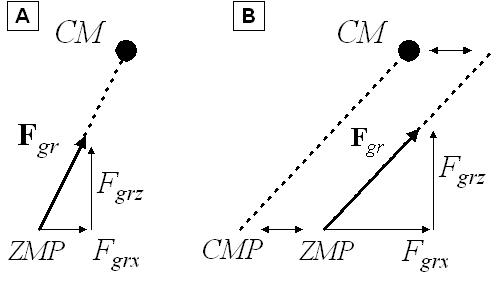
\includegraphics[height=2in]{Fig1}
\caption{As shown in A), if there is no moment about the CoM, the ground reaction force points from the ZMP to the CoM position.  As shown in  B),  if there is a moment about the CoM, the ZMP and CMP diverge, where the separation distance is the moment arm associated with the vertical force, $F_{grz}$.
(\copyright IEEE, 2009, reprinted with permission)}
\label{fig:Fig1}       
\end{figure}

The relationship between the CoM and CMP indicates the specific effect that the net ground reaction force has on CoM translation. 
Because the observed net ground reaction force always operates at the ZMP which is within the support base, 
whenever the net ground reaction force generates no torque about the CoM, then the ZMP and CMP coincide. 
If the net ground reaction force generates torque, however, then the CMP and ZMP differ in location, and, in particular, the CMP may be outside 
the support base. 

It is sometimes desirable to have the CMP and ZMP diverge as shown in Fig. 1B so that horizontal CoM forces can be more effectively controlled.  
In this case the CMP can be displaced from the ZMP which reflects the increased ability of the net ground reaction force to 
affect translation of the CoM. 
The associated moment about the CoM generally produces undesirable effects, such as loss of upright orientation of the upper body.  
In many cases, these effects are temporary, can be managed, and are well worth the overall positive effect on CoM position and velocity.  
For example, a tightrope walker will tolerate temporary angular instability if this means that he won’t fall off the tightrope.  

Use of the CMP is demonstrated in Figure \ref{fig:LateralDisturbanceRecovery}, which depicts recovery from a lateral disturbance.  
This sequence shows an initial disturbance that pushes the biped to the right.  
To compensate, the system takes control actions involving rotation of the body and swing leg, that move its CMP to the right, 
creating a lateral compensating force to the left.  
Because the disturbance is significant, the CMP moves beyond the edge of the support polygon, and thus, it does not coincide with the ZMP.  
This compensating action corresponds to a clockwise torque about the CoM, which is manifested by clockwise rotation of the torso and right leg.  

\begin{figure}%[b]
\centering
 \subfigure[]
    {
       \label{fig:LateralDisturbance1}
       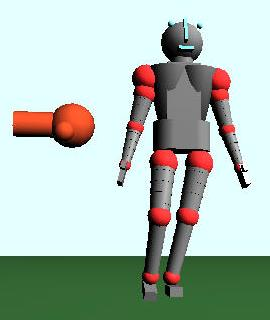
\includegraphics[height=2.5in]{LateralDisturbance1}
    }
 \subfigure[]
   {
       \label{fig:CMP_recovery1}
       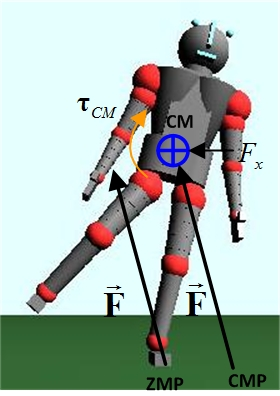
\includegraphics[height=2.5in]{CMP_recovery1}
   }\vspace{-10pt}
\caption{Recovery from a lateral disturbance using CMP.}
\label{fig:LateralDisturbanceRecovery}
\end{figure}

The model of balance control presented here, where requirements for balance are expressed in terms of CoM, ZMP, CMP, and the support base 
is extremely useful for planning and control, due to its simplicity.  
Balance control is then reduced to a problem of adjusting the base of support, adjusting the ZMP within the base of support, and, if necessary, performing motions 
that generate angular momentum, so that the CMP can be moved, temporarily, outside the base of support, in order to exert additional compensating force on the CoM.


\subsubsection{Biped Model}

Consider the three-dimensional humanoid biped model, shown in Fig. \ref{fig:BipedModel}.
The model has 7 segments:  two feet, two lower leg segments, two upper leg segments, and a body segment that lumps the torso, head, and arms.  
The leg and body segments are modeled as cylinders, whereas the feet are modeled as rectangular blocks.  
Segment dimensions and masses are given in Tables \ref{tab:ModelSegmentMasses} and \ref{tab:ModelSegmentDimensions}.  
Twelve degrees of freedom correspond to joints (6 in each leg), and 6 degrees of freedom correspond to upper body position and orientation.  
Each leg is modeled with a ball-and socket hip joint (3 degrees of freedom), a pin knee joint (one degree of freedom), and a saddle-type ankle joint 
(two degrees of freedom).  
Note that although the humanoid model presented here does not include independently moving arms, the model, and the DVMC control architecture 
can be easily extended to include them.    

\begin{figure}[b]
% \sidecaption
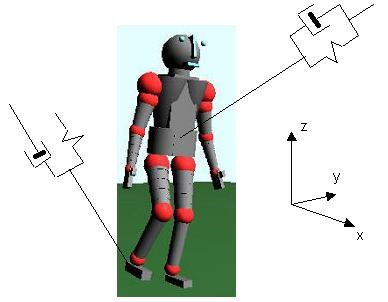
\includegraphics[height=2.2in]{BipedModel}
\caption{Virtual linear spring-damper elements, attached to reaction points, allow the mechanism to be controlled as if it were a puppet.  
The coordinate frame is as follows: x is the anterior-posterior axis, y is the medio-lateral axis, and z is the vertical axis.
(\copyright IEEE, 2009, reprinted with permission)}
\label{fig:BipedModel}       
\end{figure}

The outputs to be controlled are listed in Table \ref{tab:ControlOutputs}.  
These outputs are values relevant to balance control and locomotion, such as CM position, upper body orientation, and stepping foot position.  
Thus, the purpose of the DVMC is to move the joints so that the desired motion for the outputs is achieved.  

\begin{table}
\caption{Model Segment Masses}
\label{tab:ModelSegmentMasses}   

\begin{tabular}{p{3cm}p{3cm}}
\hline\noalign{\smallskip}
Model Segment & Mass (kg) \\
%\noalign{\smallskip}\svhline
\noalign{\smallskip} \hline
Foot & 1.56\\
Lower Leg & 4.48\\
Upper Leg & 10.73\\
Upper Body & 70.65\\
\noalign{\smallskip}\hline\noalign{\smallskip}
\end{tabular}
% $^a$ Table foot note (with superscript)
\end{table}



\begin{table}
\caption{Model Segment Dimensions}
\label{tab:ModelSegmentDimensions}  

\begin{tabular}{p{3cm}p{3cm}p{3cm}}
\hline\noalign{\smallskip}
Model Segment & Length (m) & Radius (m) \\
\noalign{\smallskip} \hline
Upper Body & 0.64 & 0.18\\
Upper Leg & 0.46 & 0.08\\
Lower Leg & 0.48 & 0.05\\
Hip Spacing & 0.25\\
\noalign{\smallskip}\hline\noalign{\smallskip}
\end{tabular}
% $^a$ Table foot note (with superscript)
\end{table}



\begin{table}
\caption{Outputs to be Controlled}
\label{tab:ControlOutputs}   

\begin{tabular}{p{3cm}p{8.5cm}}
\hline\noalign{\smallskip}
Index & Output \\
\noalign{\smallskip} \hline
1 & Posterior-anterior CM position\\
2 & Medio-lateral CM position\\
3 & Vertical CM position\\
4 & Upper body roll angle\\
5 & Upper body pitch angle\\
6 & Upper body yaw angle\\
7 & Posterior-anterior swing foot position\\
8 & Medio-lateral swing foot position\\
9 & Vertical swing foot position\\
10 & Swing foot roll angle\\
11 & Swing foot pitch angle\\
12 & Swing foot yaw angle\\
\noalign{\smallskip}\hline\noalign{\smallskip}
\end{tabular}
$^a$ For single-support case, in the global coordinate frame.  For double-support, outputs 7-12 (the ones associated with the swing foot) are omitted.
\end{table}


\subsubsection{Controller Architecture}

Desired motion behavior for the outputs is specified in a simple, straightforward way, using a linear proportional-differential (PD) law:

\begin{equation}
\ddot{\mathbf{y}} = \mathbf{k}_s \left( \mathbf{y}_s - \mathbf{y}\right) + \mathbf{k}_d \left( \dot{\mathbf{y}}_s - \dot{\mathbf{y}}\right)
\label{eq:DesiredMotion}
\end{equation}

\noindent where $\mathbf{y}$ is the vector of outputs to be controlled, $\mathbf{y}_s$ and $\dot{\mathbf{y}}_s$ are position and velocity
setpoint vectors, and $\mathbf{k}_s$ and $\mathbf{k}_d$ are spring and damping gain vectors.
Such a control law can be represented as a set of virtual spring-damper elements attached to the output points being controlled, as shown in 
Figure \ref{fig:BipedModel}, so that the controlled outputs move as if they were point masses attached to these spring-damper systems.

The difficulty with this is that the robot is not a linear system; the accelerations of the controlled outputs are nonlinear functions of the 
joint torque actuation inputs.  
The DVMC solves this problem by providing an abstraction of the plant, shown in Figure \ref{fig:LinearizationSISO}, which makes it appear linear, and
therefore, allows it to follow control laws in the form of Eq. \ref{eq:DesiredMotion}. 

\begin{figure}[b]
% \sidecaption
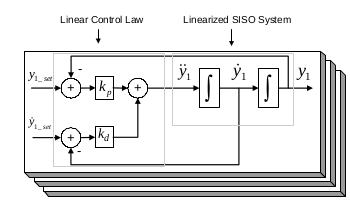
\includegraphics[height=2.2in]{LinearizationSISO}
\caption{Linear virtual element abstraction consisting of a set of SISO systems with associated linear control laws.}
\label{fig:LinearizationSISO}       
\end{figure}

This use of virtual elements is similar, in concept, to the one used in a virtual model controller \cite{pratt1997virtual}.  
However, unlike \cite{pratt1997virtual}, the DVMC accounts for plant dynamics, resulting in a linear system where controlled points move as if they were linear second order systems.  
Furthermore, through the use of a goal prioritization technique, the DVMC is able to generate moments about the CM in order to generate beneficial forces on the CM.

The DVMC uses a model-based input-output linearization algorithm \cite{slotine1991applied} to linearize and decouple the plant.  
The input-output linearization approach is augmented with a slack variable relaxation technique to accommodate actuation constraints and prioritize goals.  
This feature is important because it is not always possible to achieve all control goals simultaneously.  
Actuation constraints, such as the requirement that the ZMP must remain well inside the support base in the case where foot roll is undesireable, 
may cause the overall system to become over-constrained, in which case some goals must be deferred.  
To address this problem, the controller incorporates a goal prioritization algorithm that automatically sacrifices lower-priority goals when 
the system becomes over-constrained in this way.  
For example, the system may temporarily sacrifice goals of maintaining upright posture in order to achieve CM state goals.  
We now describe the linearization and goal prioritization components of the controller in more detail.


\subsubsection{Linear Virtual Element Abstraction}

A geometric transform, $\mathbf{h}$, is used to convert from the joint state to the workspace (output) state representation, according to

\begin{equation}
\mathbf{y} = \mathbf{h} \left( \mathbf{q} \right)
\label{eq:Kinematics}
\end{equation}

\noindent where $\mathbf{q}$ is the joint position vector, and $\mathbf{y}$ is the output vector.
Thus, $\mathbf{h}$ is the kinematic transform.
The controller uses a feedback linearizing transformation to convert desired workspace variable accelerations, $\ddot{\mathbf{y}}$, 
into corresponding joint torques.  
Application of these torques results in a new joint state, and associated workspace state.  
Use of the linearizing transformation makes the nonlinear plant appear to be a set of decoupled SISO linear 2nd-order systems, 
as shown in Figure \ref{fig:LinearizationSISO}.  
Each SISO system can then be controlled by a proportional-differential (PD) law, as discussed previously, resulting in a \textit{linear virtual element abstraction}.  

The linearization is accomplished using a two-stage process, as shown in Figure \ref{fig:TwoStageLinearization}.  
Given a desired output acceleration vector, $\ddot{\mathbf{y}}_{des}$, which is computed by the PD law, we first compute the corresponding joint acceleration vector,
$\ddot{\mathbf{q}}_{des}$, using a geometric transformation.  
Then, we compute the joint torque vector, $\tau$, that achieves $\ddot{\mathbf{q}}_{des}$, using an inverse dynamics transformation \cite{craig2005introduction}.  

The inverse dynamics computation is of the form

\begin{equation}
\mathbf{H} \left( \mathbf{q} \right) \ddot{\mathbf{q}} + \mathbf{C} \left( \mathbf{q}, \dot{\mathbf{q}} \right) + \mathbf{g} \left( \mathbf{q} \right) = \mathbf{\tau}
\label{eq:InverseDynamics}
\end{equation}

\noindent where $\mathbf{H} \left( \mathbf{q} \right)$ is a matrix of inertial terms, $\mathbf{C} \left( \mathbf{q}, \dot{\mathbf{q}} \right)$ is a
matrix of velocity-related terms, and $\mathbf{g} \left( \mathbf{q} \right)$ is a vector of gravitational terms.  
Hence, for a particular joint state $\left[ \mathbf{q}^T, \dot{\mathbf{q}}^T  \right]$, Eq. \ref{eq:InverseDynamics} represents a linear relation between
$\mathbf{\tau}$ and $\ddot{\mathbf{q}}$.
Note also that because $\mathbf{\tau}$ and $\ddot{\mathbf{q}}$ are both 12-element vectors (corresponding to the 12 actuators), 
$\mathbf{H} \left( \mathbf{q} \right)$ is a 12x12 square matrix, so Eq. \ref{eq:InverseDynamics} is fully constrained.

\begin{figure}[b]
% \sidecaption
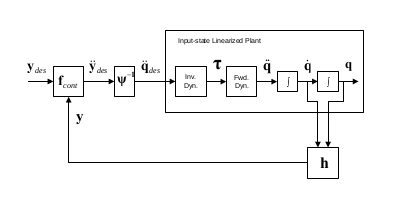
\includegraphics[height=2.2in]{TwoStageLinearization}
\caption{Two-stage Linearization}
\label{fig:TwoStageLinearization}       
\end{figure}

In order to obtain a relation between $\ddot{\mathbf{y}}_{des}$ and $\ddot{\mathbf{q}}_{des}$, 
we differentiate Eq. \ref{eq:Kinematics} twice to obtain

\begin{eqnarray}
\dot{\mathbf{y}} = \frac{\partial \mathbf{h}}{\partial \mathbf{q}} \dot{\mathbf{q}} = \mathbf{J} \dot{\mathbf{q}}\\
\ddot{\mathbf{y}} = \mathbf{J} \ddot{\mathbf{q}} + \dot{\mathbf{J}} \dot{\mathbf{q}} = \mathbf{J} \ddot{\mathbf{q}} + \Psi
\label{eq:DifferentiatedKinematics}
\end{eqnarray}

\noindent where $\mathbf{J}$ is the Jacobian matrix.
The matrix $\mathbf{J}$ and the vector $\Psi$ are functions of joint state.
Therefore, for a particular joint state $\left[ \mathbf{q}^T, \dot{\mathbf{q}}^T  \right]$, Eq. \ref{eq:DifferentiatedKinematics} represents 
a linear relation between $\ddot{\mathbf{q}}$ and $\ddot{\mathbf{y}}$.
Note also that because $\mathbf{q}$ and $\mathbf{y}$ are both 12-element vectors, Eq. \ref{eq:DifferentiatedKinematics} represents a fully constrained system.

To achieve the linearization shown in Figure \ref{fig:TwoStageLinearization}, we combine Eqs. \ref{eq:InverseDynamics} and \ref{eq:DifferentiatedKinematics}:

\begin{equation}
\begin{bmatrix}
\mathbf{I}_{12 \times 12} & \mathbf{0}_{12 \times 12} & \mathbf{0}_{12 \times 12} \\
\mathbf{I}_{12 \times 12} & - \mathbf{J} & \mathbf{0}_{12 \times 12} \\
\mathbf{0}_{12 \times 12} & \mathbf{H} & - \mathbf{I}_{12 \times 12}
\end{bmatrix}
\begin{bmatrix}
\ddot{\mathbf{y}} \\
\ddot{\mathbf{q}} \\
\mathbf{\tau} 
\end{bmatrix} = 
\begin{bmatrix}
\ddot{\mathbf{y}}_{des} \\
\Psi \\
- \mathbf{C} 
\end{bmatrix}
\label{eq:FBLin}
\end{equation}

Note that this is a fully constrained, linear system.



\subsubsection{Multivariable Optimal Controller}

The linearization of the square system represented by Eq. \ref{eq:FBLin} is subverted if inequality constraints are introduced, and these constraints become active;  
the system represented by Eq. \ref{eq:FBLin} becomes over-constrained in this case.  
Inequality constraints are used to represent actuation limits.  
An important constraint of this type is the requirement to keep the stance foot flat on the ground during single support;  
while balancing on one leg it is undesirable for the stance foot to roll, particularly on its lateral edge.  
This particular constraint is accomplished by requiring the ZMP to be inside the edge of the support envelope.  
Note that this constraint is distinct from the physical constraint that the ZMP not be outside the support base.  
If the ZMP is on the edge of the support envelope, the foot will begin to roll \cite{popovic2005ground}.  
Hence, in order to avoid foot roll, we employ linear inequality constraints to keep the ZMP inside the edge of the support envelope.

For the humanoid model, the ZMP is given by expanding Eq. \ref{eq:ZMP}, or

\begin{eqnarray}
x_{ZMP} = \frac{\sum_{i=2}^7 m_i r_{xi} \left( \ddot{r}_{zi} + g\right) - \sum_{i=2}^7 m_i r_{zi} \ddot{r}_{xi} - \sum_{i=2}^7 \tau_{yi}}
{\sum_{i=2}^7 m_i \left( \ddot{r}_{zi} + g\right)} \\
y_{ZMP} = \frac{\sum_{i=2}^7 m_i r_{yi} \left( \ddot{r}_{zi} + g\right) - \sum_{i=2}^7 m_i r_{zi} \ddot{r}_{yi} + \sum_{i=2}^7 \tau_{xi}}
{\sum_{i=2}^7 m_i \left( \ddot{r}_{zi} + g\right)} \\
\mathbf{\tau}_{xi} = \mathbf{I}_{Gi} \dot{\mathbf{\omega}_{xi}} \\
\mathbf{\tau}_{yi} = \mathbf{I}_{Gi} \dot{\mathbf{\omega}_{yi}}
\label{eq:ZMPexpanded}
\end{eqnarray}

\noindent where $i$ is the segment index, $r_{xi}$, $r_{yi}$, and $r_{zi}$ denote the CM position of segment $i$, $\mathbf{I}_{Gi}$ is the inertia matrix of 
segment $i$, and $\mathbf{\omega}_{xi}$ and $\mathbf{\omega}_{yi}$ are the angular velocities of segment $i$ about the x and y axes, respectively.
The moments, $\mathbf{\tau}_{xi}$ and $\mathbf{\tau}_{yi}$, are about the segment $i$ CM in the x and y axes, respectively.

Eq. \ref{eq:ZMPexpanded} is transformed into a set of linear inequality constraints by replacing $x_{ZMP}$ and $y_{ZMP}$ with min and max terms, reflecting 
the bounds, so that these become constants:

\begin{equation}
\mathbf{H}_r \ddot{\mathbf{y}}_r \leq \mathbf{K}_r
\label{eq:LinearInequality}
\end{equation}

\noindent where

\begin{equation}
\mathbf{H}_r = 
\begin{bmatrix}
- \mathbf{m}^T \bullet \mathbf{r}_z^T & \mathbf{0}_{1 \times 6} & \left( -\mathbf{x}_{max} + \mathbf{m}^T \bullet \mathbf{r}_x^T \right) & \mathbf{0}_{1 \times 6} & - \mathbf{I}_y \\
\mathbf{m}^T \bullet \mathbf{r}_z^T & \mathbf{0}_{1 \times 6} & \left( \mathbf{x}_{min} - \mathbf{m}^T \bullet \mathbf{r}_x^T \right) & \mathbf{0}_{1 \times 6} & \mathbf{I}_y \\
\mathbf{0}_{1 \times 6} & - \mathbf{m}^T \bullet \mathbf{r}_z^T & \left( -\mathbf{y}_{max} + \mathbf{m}^T \bullet \mathbf{r}_y^T \right) & \mathbf{I}_x & \mathbf{0}_{1 \times 6} \\
\mathbf{0}_{1 \times 6} & \mathbf{m}^T \bullet \mathbf{r}_z^T & \left( \mathbf{y}_{min} - \mathbf{m}^T \bullet \mathbf{r}_y^T \right) & - \mathbf{I}_x & \mathbf{0}_{1 \times 6}
\end{bmatrix}
\label{eq:Hr_def}
\end{equation}

\begin{equation}
\ddot{\mathbf{y}}_r = 
\begin{bmatrix}
\ddot{\mathbf{r}}_x^T & \ddot{\mathbf{r}}_y^T & \ddot{\mathbf{r}}_z^T & \dot{\mathbf{\omega}}_x^T & \dot{\mathbf{\omega}}_y^T
\end{bmatrix}^T
\label{eq:yr_def}
\end{equation}

\begin{equation}
\mathbf{K}_r = 
\begin{bmatrix}
g \left( m_{tot} x_{zmpmax} - \mathbf{m}^T \bullet \mathbf{r}_x^T \right)^T \\
-g \left( m_{tot} x_{zmpmin} - \mathbf{m}^T \bullet \mathbf{r}_x^T \right)^T \\
g \left( m_{tot} y_{zmpmax} - \mathbf{m}^T \bullet \mathbf{r}_y^T \right)^T \\
-g \left( m_{tot} y_{zmpmin} - \mathbf{m}^T \bullet \mathbf{r}_y^T \right)^T \\
\end{bmatrix}
\label{eq:Kr_def}
\end{equation}

\begin{eqnarray}
\mathbf{x}_{max} = x_{zmpmax} \mathbf{m}^T\\
\mathbf{x}_{min} = x_{zmpmin} \mathbf{m}^T\\
\mathbf{y}_{max} = y_{zmpmax} \mathbf{m}^T\\
\mathbf{y}_{min} = y_{zmpmin} \mathbf{m}^T
\label{eq:SupportLimits}
\end{eqnarray}

\noindent where $\mathbf{m}$ is a 6-element vector of masses for segments 2 – 7, $\mathbf{r}_x$, $\mathbf{r}_y$, and $\mathbf{r}_z$ 
are 6-element vectors of the segments’ CM x, y, and z positions, $\mathbf{I}_x$ and $\mathbf{I}_y$ are 6-element vectors of the segments’ inertias 
about the x and y axes, and $x_{zmpmin}$, $x_{zmpmax}$, $y_{zmpmin}$, and $y_{zmpmax}$ are the ZMP limits.  The operator $\bullet$ represents element-wise multiplication.

Now, $\mathbf{r}_x$, $\mathbf{r}_y$, $\mathbf{r}_z$, $\mathbf{I}_x$ and $\mathbf{I}_y$ are kinematic functions of $\mathbf{q}$, and $\mathbf{m}$ is a constant.
Therefore, Eq. \ref{eq:LinearInequality} is linear with respect to the current joint state.  
Furthermore, $\ddot{\mathbf{y}}_r$ is related to the joint acceleration vector through a linear function similar to Eq. \ref{eq:FBLin}:

\begin{equation}
\ddot{\mathbf{y}}_r = \mathbf{J}_r \ddot{\mathbf{q}} + \Psi_r
\label{eq:yr_def2}
\end{equation}

\noindent Therefore, if we combine the inequality constraints of Eq. \ref{eq:yr_def2} with \ref{eq:LinearInequality}, we have an overall system that is either 
fully constrained or over constrained (because $\ddot{\mathbf{y}}_r$ is fully dependent on $\ddot{\mathbf{q}}$, it does not add any flexibility).  
If none of the constraints in Eq. \ref{eq:LinearInequality} are active, the system is fully constrained.  
However, if one of these constraints is active, the system becomes over constrained, and there is no feasible solution.  
Consequently, if the controller does not take the constraints in Eq. \ref{eq:LinearInequality} into consideration, it could generate values for $\ddot{\mathbf{y}}_{des}$
that are infeasible.

One way to avoid this type of infeasibility is to use “slack” variables that provide flexibility to the overall system.  
Thus, the controller output, $\ddot{\mathbf{y}}_{contout}$, is given by

\begin{equation}
\ddot{\mathbf{y}}_{des} = \ddot{\mathbf{y}}_{contout} + \ddot{\mathbf{y}}_{slack}
\label{eq:y_contout}
\end{equation}

\noindent where $\ddot{\mathbf{y}}_{slack}$ is the vector of slack variables.  
The goal of the overall control system is then to minimize $\ddot{\mathbf{y}}_{slack}$, taking into account the relative importance of each element.  

This minimization is accomplished by formulating the control problem as a quadratic program (QP), and then using a QP optimizer to solve it.  
The relative importance of the slack variables is expressed in the cost function for the QP.
This causes the optimizer to prioritize goals by first minimizing the slack variables for the most important outputs, and therefore, setting
$\ddot{\mathbf{y}}_{contout}$ to be as close as possible to $\ddot{\mathbf{y}}_{des}$ for these outputs.  
For example, slack variables associated with the CM position output are given higher cost than those associated with trunk and swing leg orientation.  
The slack variable costs were determined empirically.  
Their precise value is not crucial;  as long as the slack costs for CM position are higher than the slack costs for the other outputs, desired behavior is achieved.

The QP formulation is under-constrained, due to the use of the slacks.  
The QP optimizer explores the null space of the formulation, choosing the solution that minimizes the cost function.  
This cost function is of the form $\mathbf{w} \cdot \ddot{\mathbf{y}}_{slack}$ where $\mathbf{w}$ 
is a vector of weights reflecting the importance of minimizing the associated slack variable \cite{hofmann2004sliding}. 






%%%%%%%%%%%%%%%%%%%%%%%%%%%%%%%%%%%%%%%%%%%%%%%%%%%%%%%%%%%%%%%%%%%%%%%%%%%%%%%
\subsection{Momentum-Based Computed Torque Control }
\label{sec:framework}
%%%%%%%%%%%%%%%%%%%%%%%%%%%%%%%%%%%%%%%%%%%%%%%%%%%%%%%%%%%%%%%%%%%%%%%%%%%%%%%


\begin{figure}[h]
\begin{center}
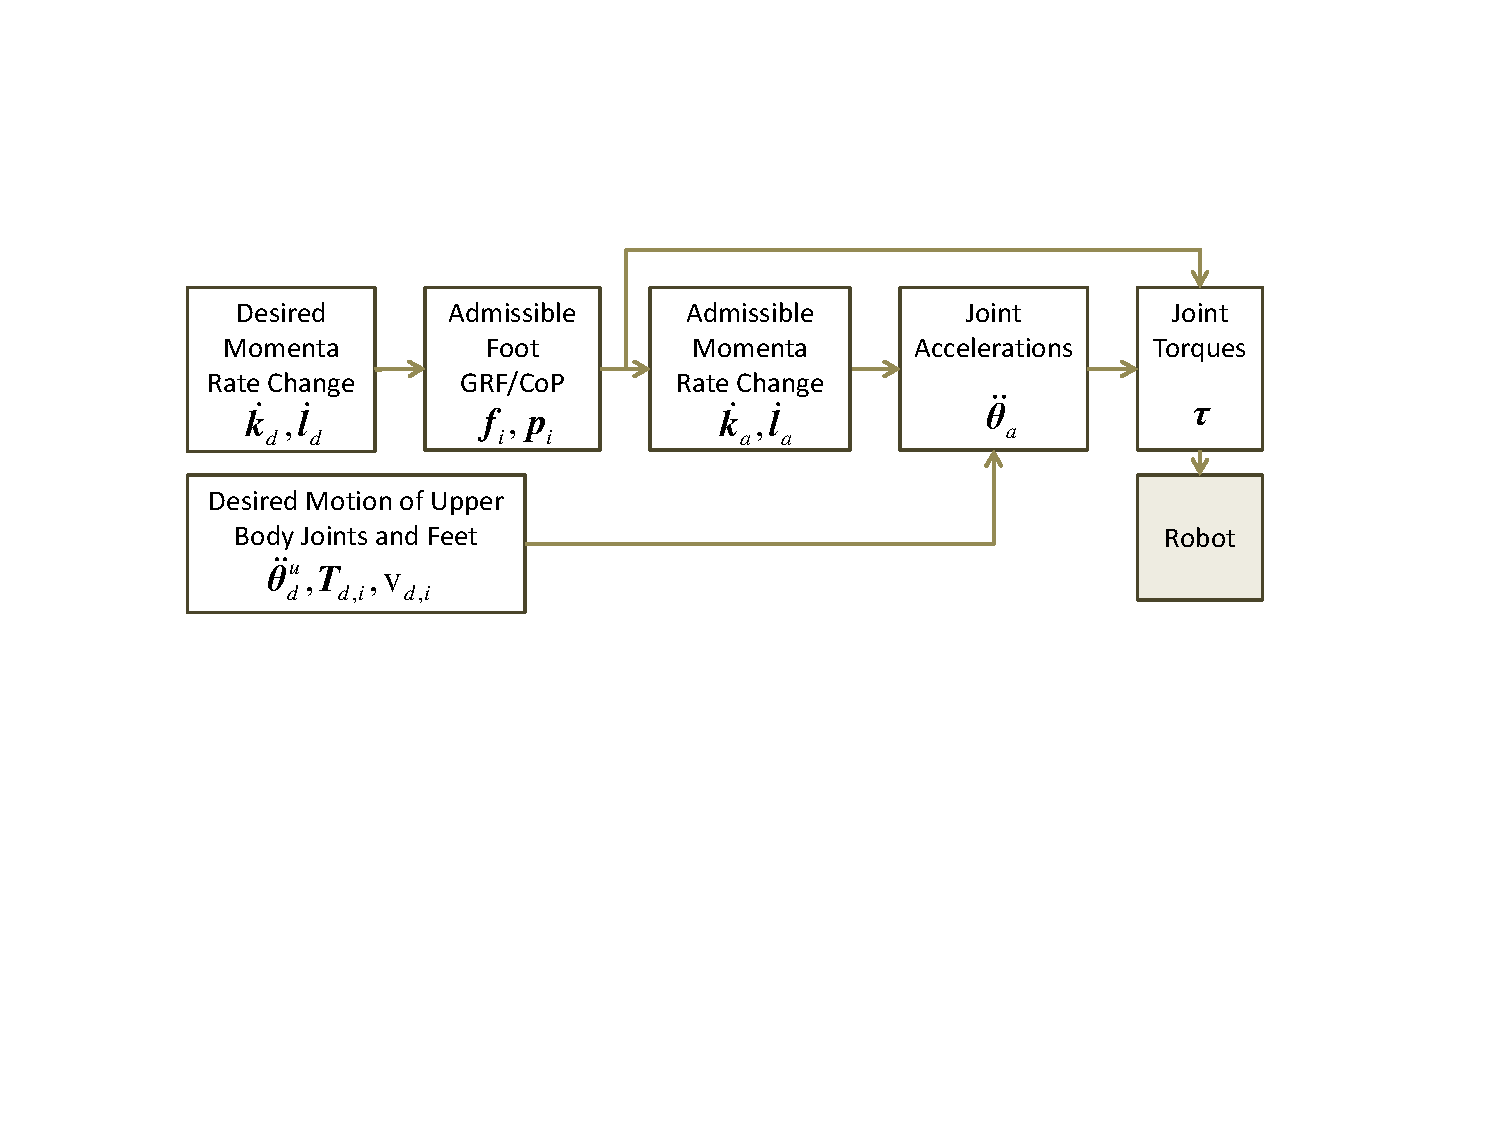
\includegraphics[width = 0.7\columnwidth]{Figures/diagram-short.pdf}
\end{center}
\caption{Overview of momentum-based balance controller introduced in~\cite{LG12}.
$\vddth_d^u$ is the desired joint accelerations for the upper body.
$\mT_{d,i}$ and $\sv_{d,i}$ are the desired configuration
and spatial velocity of each foot ($i = r, l$). Subscripts $d$ and $a$ imply {\em ``desired''} and {\em ``admissible,''} respectively. }
\label{fig:overview}
\end{figure}


Some momentum-based balance control approaches define the desired rotational
behavior of the controller in terms of the CoP~\cite{AG05,Macchietto09}
while others use angular momentum~\cite{KKKFHYH03}.
Although the GRF-CoP combination has a one-to-one relationship
with momentum rate changes, their significance regarding
balance are different: Whereas the former characterize the magnitude, direction and
point of application of
the external forces, the latter describes the resulting motion of a robot.
The unilateral nature of robot-ground contact and friction limits
impose important direct constraints on the range of GRF and CoP.
 These influence the achievable range of momentum rate change,
 but only indirectly. On the other hand, it is more natural to describe
the aggregate motion of a robot in terms of momentum.


In this chapter we present a momentum-based balance controller developed in~\cite{LG12}
that uses momentum to define control objectives as well as to compute joint motions
while GRF and CoP are used as constraints.
Fig.~\ref{fig:overview} shows the block diagram for the controller.
In this method, the desired momentum rate change for balance is first specified.
However, the desired momentum rate change may not always be physically
realizable due to several constraints on the foot-ground
contact. First, the CoP cannot be outside the
robot's support base.\footnote{ During single support, the support base is identical to
the foot contact area, whereas during double support on level ground,
the support base is equivalent to the
convex hull of the support areas of the two feet.}
Second, the GRF must be unilateral in nature, and can never attract the
robot towards the ground. Third, the GRF must satisfy the friction
limit of the foot-ground surface, so as not to cause slip.

Therefore, the next step determines the admissible values of GRF
and CoP that will create the desired momentum rate change as close
as possible while being physically realizable.
Specifically, in order to make the controller robustly applicable to non-level
and non-stationary ground, admissible \emph{foot} GRFs and \emph{foot} CoPs
ared directly determined,
without using more conventional \emph{net} GRF and \emph{net} CoP of the robot.
Assuming planar contact between the ground and each foot, the foot GRF is the ground
reaction force acting on an individual foot and foot CoP
is the location where its line of action intersects the foot
support plane.
Using the values of admissible foot GRF and foot CoP 
momentum rate changes are recalculated -- these are the \emph{admissible} momentum rate changes.

The subsequent step resolves the joint accelerations given
the admissible momentum rate change, desired joint accelerations for the upper body,
and desired motion of the feet.
Finally necessary joint torques are computed to create
the joint accelerations and the admissible external forces
using inverse dynamics.


During double support, the computation of foot GRFs and foot CoPs
from the desired momentum rate change is an under-determined problem. This
allows for pursuing an additional optimality criterion in the solution.
For example, the ankle torques can be minimized while generating
the desired momentum rate change.
Minimizing ankle torque is important because
typically the ankle torque is more constrained than
others in that it should not cause foot tipping.

%The main unique contributions of this paper can be listed as follows:
%\begin{enumerate}
%\item Our momentum-based control framework determines the desired momenta but before attempting to reach them, it first checks to make sure that the momenta targets are physically attainable by computing their admissible values.
%\item The optimal foot GRFs and foot CoPs are computed quickly by solving two small-scale linear least-squares problems.
%\item The framework is sufficiently general to support a momentum-based stepping algorithm, as reported recently~\cite{YG11}.
%\end{enumerate}


%===================================================
%\subsection{Control Framework}
%\label{sec:control_framework2}
%===================================================

%We will represent the configuration of a humanoid robot as $Q=(\mT_0,\vth)\in\SE\times\real^n$, where $\mT_0=(\mR_0 ,\vp_0) \in \SO\times\real^3$ denotes the base frame (trunk) configuration, $\vth\in \real^n$ is the vector of joint angles, and $n$ is the total number of joint DoFs.
%The subscripts $0$ and $s$ denote the base frame and joints, respectively, with $s$ implying ``shape'' associated with the joint angles in geometric dynamics~\cite{Block96}. The total DoFs of the robot is thus $6+n$, because the floating base has $6$ DoFs. The generalized velocity can be written as $\vdq=(\sv_0,\vdth)\in \real^{6+n}$ where $\sv_0 = (\vom_0,\vup_0)$ is the spatial velocity of the trunk with respect to the body frame and expressed as:
%\footnote{$\vdq$ is a slight abuse of notation because we do not define nor use a vector $\vq$. However, since $\se$, the Lie algebra of $\SE$, is isomorphic to $\real^6$, we will use a single vector form of $\vdq\in\real^{6+n}$ for convenience. $\skewsym{\vom_0}$ represents a skew-symmetric matrix of a vector $\vom_0$.}
%\begin{align}
%\skewsym{\vom_0} &= \mR_0^T \boldsymbol{\dot{R}}_0 \\
%\vup_0 &= \mR_0^T \boldsymbol{\dot{p}}_0
%\end{align}
%Then, a

Let us review the above framework in terms of the equations of motion of a robot.
Assuming stationary ground, the constraint equations due to ground contacts and
the joint space equations of motion of the robot are as follows:
\begin{align}
	\vzero &= \mJ_c \vdq\label{eq:constraint}	\\
	\vtau &= \mH \vddq + \mC\vdq + \vtau_g - \mJ_c^T\vf_c \label{eq:joint_space_eom}
\end{align}	
where $\vtau \in \real^{n}$ denotes the generalized forces,
$\mH$ is the joint space inertia matrix, $\mC\vdq$ includes Coriolis and centrifugal terms
and $\vtau_g$ is the gravity torque.
$\vf_c$ is a vector representing external ``constraint'' forces from the ground,
determined by foot GRFs and CoPs, and the Jacobian $\mJ_c\in\real^{c\times n}$ transforms $\vf_c$ to the generalized forces. The number of constraint equations $c$ depends on the nature of constraint at the foot-ground contact.
For example, when both the linear and angular motion of the support foot are constrained due to foot-ground contact,
$c=6$ for single support and $c=12$ for double support. In this case, $\mJ_c\vdq$ denotes
the linear and angular velocities of the support foot given $\vdq$, and $\vzero$ in (\ref{eq:constraint})
denotes zero velocity of the support foot.


Since the robot base is free floating, the first six elements of $\vtau$ are zero,
i.e., $\vtau^T = [ \vec{0}^T~ \vtau_s^T ]$.
Hence, we can divide (\ref{eq:joint_space_eom}) into two parts, one corresponding to the base, denoted by the subscript 0, and the other, subscripted with $s$, for the joints.
Then (\ref{eq:constraint}) and (\ref{eq:joint_space_eom}) are rewritten as follows:
\begin{align}
	\vzero &= \mJ_c\vddq + \mdJ_c \vdq \label{eq:const1}\\
	\vzero &= \mH_0 \vddq + \mC_0\vdq  + \vtau_{g,0} - \mJ_{c,0}^T \vf_c \label{eq:eom_base}\\
	\vtau_s &= \mH_s \vddq + \mC_s\vdq  + \vtau_{g,s} - \mJ_{c,s}^T\vf_c \label{eq:eom_joint}
\end{align}
where (\ref{eq:const1}) is the time derivative of (\ref{eq:constraint}).
%(?? according to the order of eqs 4 and 5, eqs. 7 and 8 should come before eq. 6)
%(?? the "dot" on italics J is shifted too much to the left)==>can't figure our how to fix it.

%Due to the high DoFs of humanoid robots, balance controllers usually solve an optimization problem. However, the computational cost of the optimization increases rapidly as the dimension of the search space increases. Even the simplest optimization problem such as the least-squares problem has order $O(n^3)$ time complexity.
%Therefore, aiming for computational efficiency, we have adopted a sequential approach; we divide the balance control problem into three smaller sub-problems, which can be solved serially.
The balance controller determines the control input $\vtau_s$
through the following steps:
%by sequentially determining $\vf$, $\vddq$, and $\vtau_s$, in that order.
\begin{itemize}
	\item {\bf Step 1}: foot GRFs and foot CoPs (hence $\vf_c$) are computed
	   from the desired momentum rate change.
	\item {\bf Step 2}: joint accelerations $\vddq$ are determined
	   such that they satisfy both (\ref{eq:const1}) and (\ref{eq:eom_base}).
        Actually, as will be explained in Sec.~\ref{sec:joint_acc}, instead of
        directly using (\ref{eq:eom_base}), we use the centroidal momentum
        equation (\ref{eq:hGdot}), which is equivalent to (\ref{eq:eom_base}). In general, if the total number of robot DoFs is greater
        than or equal to $c+6$, a solution to $\vddq$ exists.
	\item {\bf Step 3}: the required joint torques $\vtau_s$ satisfying
	   (\ref{eq:eom_joint}) are computed from $\vf_c$ and $\vddq$ using
        an inverse dynamics algorithm.
	\label{it:steps}
\end{itemize}

Note that, by computing $\vf_c$ and $\vddq$ first,
we can use efficient linear-time algorithms for inverse dynamics in {\bf Step 3},
without having to compute the joint space equations of motion (\ref{eq:joint_space_eom})
which have a quadratic time complexity.


%%%%%%%%%%%%%%%%%%%%%%%%%%%%%%%%%%%%%%%%%%%%%%%%%%%%%%%%%%%%%%%%%%%%%%%%%%%%%%%
%\subsection{Single Support}
%%%%%%%%%%%%%%%%%%%%%%%%%%%%%%%%%%%%%%%%%%%%%%%%%%%%%%%%%%%%%%%%%%%%%%%%%%%%%%%

%%%%%%%%%%%%%%%%%%%%%%%%%%%%%%%%%%%%%%%%%%%%%%%%%%%%%%%%%%%%%%%%%%%%%%%%%%%%%%%
%\subsection{Double Support}
%%%%%%%%%%%%%%%%%%%%%%%%%%%%%%%%%%%%%%%%%%%%%%%%%%%%%%%%%%%%%%%%%%%%%%%%%%%%%%%

%%%%%%%%%%%%%%%%%%%%%%%%%%%%%%%%%%%%%%%%%%%%%%%%%%%%%%%%%%%%%%%%%%%%%%%%%%%%%%%
%\subsection{Level and non-level surface}
%%%%%%%%%%%%%%%%%%%%%%%%%%%%%%%%%%%%%%%%%%%%%%%%%%%%%%%%%%%%%%%%%%%%%%%%%%%%%%%

%%%%%%%%%%%%%%%%%%%%%%%%%%%%%%%%%%%%%%%%%%%%%%%%%%%%%%%%%%%%%%%%%%%%%%%%%%%%%%%
%\subsection{Arbitrary stationary surface}
%%%%%%%%%%%%%%%%%%%%%%%%%%%%%%%%%%%%%%%%%%%%%%%%%%%%%%%%%%%%%%%%%%%%%%%%%%%%%%%

%%%%%%%%%%%%%%%%%%%%%%%%%%%%%%%%%%%%%%%%%%%%%%%%%%%%%%%%%%%%%%%%%%%%%%%%%%%%%%%
%\subsection{Moving surface (bus, moving walkway, boat)}
%%%%%%%%%%%%%%%%%%%%%%%%%%%%%%%%%%%%%%%%%%%%%%%%%%%%%%%%%%%%%%%%%%%%%%%%%%%%%%%

%%%%%%%%%%%%%%%%%%%%%%%%%%%%%%%%%%%%%%%%%%%%%%%%%%%%%%%%%%%%%%%%%%%%%%%%%%%%%%%
%\subsection{Estimation of CoM and reaction point movement state}
%%%%%%%%%%%%%%%%%%%%%%%%%%%%%%%%%%%%%%%%%%%%%%%%%%%%%%%%%%%%%%%%%%%%%%%%%%%%%%%


%%%%%%%%%%%%%%%%%%%%%%%%%%%%%%%%%%%%%%%%%%%%%%%%%%%%%%%%%%%%%%%%%%%%%%%%%%%%%%%
%%%%%%%%%%%%%%%%%%%%%%%%%%%%%%%%%%%%%%%%%%%%%%%%%%%%%%%%%%%%%%%%%%%%%%%%%%%%%%%
\section{Scenarios}
\label{sec:scenarios}
%%%%%%%%%%%%%%%%%%%%%%%%%%%%%%%%%%%%%%%%%%%%%%%%%%%%%%%%%%%%%%%%%%%%%%%%%%%%%%%
%%%%%%%%%%%%%%%%%%%%%%%%%%%%%%%%%%%%%%%%%%%%%%%%%%%%%%%%%%%%%%%%%%%%%%%%%%%%%%%

%%%%%%%%%%%%%%%%%%%%%%%%%%%%%%%%%%%%%%%%%%%%%%%%%%%%%%%%%%%%%%%%%%%%%%%%%%%%%%%
\subsection{Stationary Balance}
%%%%%%%%%%%%%%%%%%%%%%%%%%%%%%%%%%%%%%%%%%%%%%%%%%%%%%%%%%%%%%%%%%%%%%%%%%%%%%%

In this section, we show how the momentum control framework introduced in Sec.~\ref{sec:framework} is employed to create stationary balance.

%===================================================
\paragraph{Determination of the Desired Momentum:}
\label{sec:obj_bal_con}
%===================================================

The overall behavior of the robot against external perturbations
is determined by the desired momentum rate change.
For the stationary balance, the following feedback control policy can be used:
\begin{align}
	\vdk_d &= \mGamma_{11} (\vk_d - \vk) \label{eq:desAngM}\\
	\vdl_d/m &= \mGamma_{21}(\vdr_{G,d}-\vdr_G) + \mGamma_{22}(\vr_{G,d}-\vr_G) \label{eq:desLinM}
\end{align}
where $\vdk_d$ and $\vdl_d$ are the independently specified
desired rates of change of centroidal angular and
linear momenta. In other words $\vdk_d$ and $\vdl_d$ are not time derivatives of $\vk_d$ and $\vl_d$.
Additionally, $\vr_{G,d}$ is the desired CoM position.
$\mGamma_{ij}$ represents 3$\times$3 diagonal matrix of feedback gain parameters.
Note that unlike the linear position feedback term in (\ref{eq:desLinM}), an angular position
feedback is omitted in (\ref{eq:desAngM}). This is because a physically meaningful angular
``position''
cannot be defined corresponding to angular momentum\cite{Wie05}.
For postural balance maintenance experiments we set $\vk_d$ and $\vdr_{G,d}$ to zero
and $\vr_{G,d}$ to be above the mid-point of the geometric centers of the
two feet. For other cases, these values may be determined from the desired motion.

It is to be noted that, despite the various studies on angular momentum in humanoid motions,
the issue of how to set the desired angular momentum for more complex motions such as locomotion has not been fully explored, and remains an important
future work.

%===================================================
\paragraph{Prioritization between Linear and Angular Momenta:}
\label{sec:prioritization}
%===================================================

\begin{figure}[h]
\begin{center}
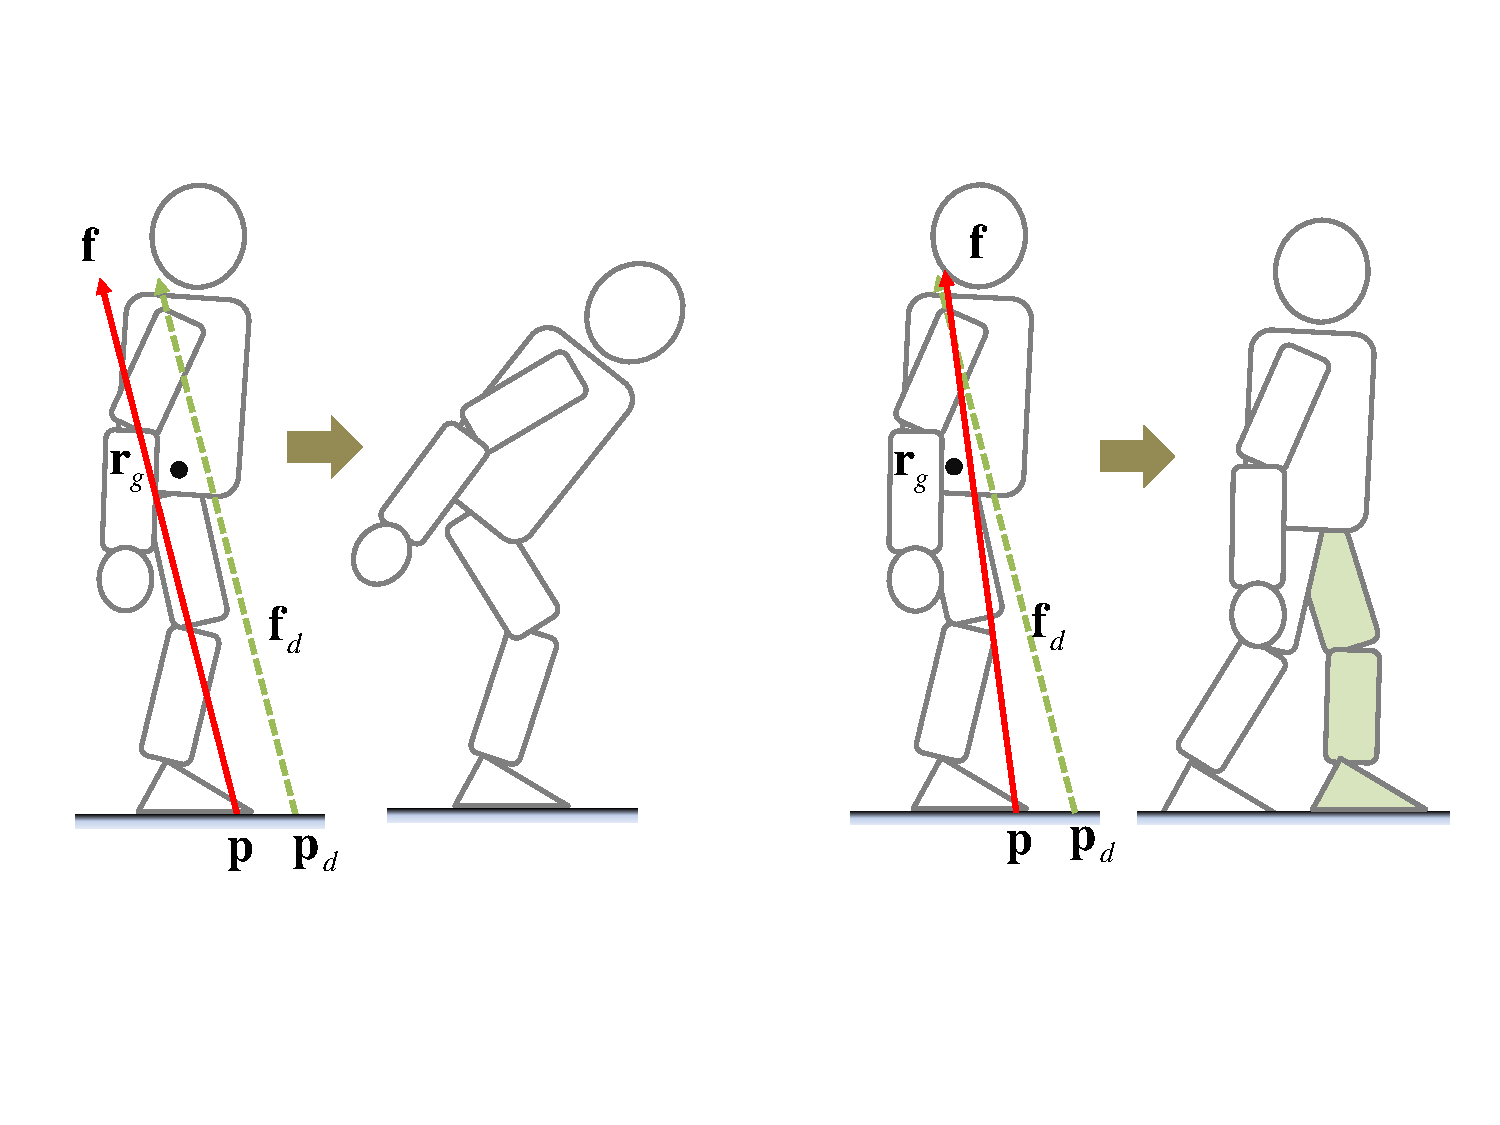
\includegraphics[width = 0.6\columnwidth]{Figures/two_cases_new.pdf}
\end{center}
\caption{
When the desired GRF, $\vf_d$ and the desired CoP, $\vp_d$ computed from
the desired momentum rate change are not simultaneously admissible,
as indicated by $\vp_d$ being outside the support base,
momenta objectives need to be compromised for control law formulation.
Two extreme cases are illustrated.
Left: linear momentum is respected while angular momentum is compromised.
Right: angular momentum is respected while linear momentum is compromised.
%A solution between the two extreme strategies could be used as well.
}
\label{fig:two_cases}
\end{figure}

Given the desired momentum rate change, 
admissible foot GRF and foot CoP are determined such that the resulting momentum
rate change is as close as possible to the desired value.
If the desired GRF and CoP computed from $\vdk_d$ and $\vdl_d$
violate physical constraints (e.g., GRF being outside friction cone,
normal component of GRF being negative, or CoP being
outside support base), it is not possible
to generate those $\vdk_d$ and $\vdl_d$. In this case we must strike
a compromise and decide which quantity out of $\vdk_d$ and $\vdl_d$ is more
important to preserve.

Fig.~\ref{fig:two_cases} illustrates one case where the desired CoP, $\vp_d$,
computed from the desired momentum rate change is outside the support base,
indicating that it is not admissible.
Two different solutions are possible.
The first solution, shown in Fig.~\ref{fig:two_cases}, left, is to translate the CoP to the closest
point of the support base while keeping the magnitude and line of action of the
desired GRF $\vf_d$ unchanged. In this case the
desired linear momentum is attained but the desired
angular momentum is compromised. The behavior emerging from this choice
is characterized by a trunk rotation. This strategy can be observed in the
human when the trunk yields in the direction of the push to maintain balance.
Alternatively, in addition to
translating the CoP to the support base, as before, we can rotate
the direction of the GRF, as shown in Fig.~\ref{fig:two_cases}, right. In this case the desired
angular momentum is
attained while the desired linear momentum
 is compromised. With this strategy
 the robot must move linearly along the direction of the applied force
due to the residual linear momentum, making it necessary to step forward
to prevent falling.

For the stationary balance, it is natural to give higher priority to preserving linear momentum over angular
momentum because it increases the capability of postural balance without
involving a stepping.
Ideally, a smart controller should be able to choose
optimal strategies depending on the environment conditions
and the status of the robot.
The approaches that give higher priority to linear
momentum and sacrifice angular momentum can also be found
in the literature~\cite{Hofmann09,Stephens10} and in our recent work on stepping~\cite{YG11}.

%===================================================
\paragraph{Admissible Foot GRF, Foot CoP, and Momentum Rate Change:}
\label{sec:local_grf}
%===================================================

Given the desired momentum rate change, admissible foot GRF and CoP are determined such that the resulting momentum
rate change is as close as possible to the desired value.
Admissible momentum rate change is determined by
the admissible foot GRF and foot CoP.

{\bf Single Support Case:}
Dealing with single support case is straightforward
because the foot GRF and CoP are uniquely determined
from the desired momentum rate change, from (\ref{eq:vdk}) and (\ref{eq:vdl}):
\begin{align}
  \vf_d &= \vdl_d - m\vg \label{eq:vf_d}\\
	p_{d,X} &= r_{G,X} - \frac{1}{\vdl_{d,Y} - mg} ( f_{d,X}\: r_{G,Y} - \dot{k}_{d,Z} )\label{eq:pdx}\\
	p_{d,Z} &= r_{G,Z} - \frac{1}{\vdl_{d,Y} - mg} ( f_{d,Z}\: r_{G,Y} + \dot{k}_{d,X} ) \label{eq:pdz}
\end{align}
where the Y-axis is parallel to the direction of gravity vector, i.e., $\vg=(0,g,0)$.

If $\vf_d$ and $\vp_d$ computed above are valid, then these
values are directly used. Otherwise, as mentioned previously, higher priority is given to linear
momentum. If $\vf_d$ is outside the friction cone, it is projected
onto the friction cone to prevent foot slipping.

{\bf Double Support Case:}
Determining foot GRFs and foot CoPs for double support is more involved. We refer the readers to the original paper~\cite{LG12} for details.



%===================================================
\paragraph*{Admissible Momentum Rate Change:}
%===================================================
After determining admissible foot GRF and foot CoP, the admissible
momentum rate change $\vdh_a=[\vdk_a^T~\vdl_a^T]^T$ is also computed
using (\ref{eq:vdk}) and (\ref{eq:vdl}) for single support, or (\ref{eq:vdk2}) and (\ref{eq:vdl2})
for double support.

%===================================================
\paragraph{Determination of Joint Accelerations and Torques:}
\label{sec:joint_acc}
%===================================================

After determining the admissible foot GRFs and foot CoPs, and admissible momentum
rate changes, we compute joint accelerations and torques
to realize them similarly to~\cite{Macchietto09}.

%First, we resolve the desired joint accelerations  $\vddq$ for balance such that they satisfy (\ref{eq:const1}) and a variation of (\ref{eq:eom_base}).
%To explain the latter let us first express the spatial centroidal momentum $\vh=[\vk^T~\vl^T]^T$ in terms of the generalized velocities:
%\begin{equation}
%	\vh = \mA(Q) \vdq   \, ,\label{eq:cmm1}
%\end{equation}
%where $\mA\in\real^{6\times (6+n)}$ is the centroidal momentum matrix~\cite{OG08} that linearly maps the generalized velocities to the spatial momentum. Differentiating (\ref{eq:cmm1}), we obtain
%\begin{equation}
%	\vdh = \mA \vddq + \mdA\vdq  \, .\label{eq:cmm}
%\end{equation}

%If we replace $\vdh$ with external forces  using Newton's law (refer to (\ref{eq:vdk}) and (\ref{eq:vdl})), then (\ref{eq:cmm}) expresses the aggregate motion of the dynamic system due to the external forces, which is exactly same as what (\ref{eq:eom_base}) represents. Note that the joint torques are not included in (\ref{eq:eom_base}). The only difference is the reference frame: (\ref{eq:cmm}) is expressed with respect to a frame at the CoM whereas (\ref{eq:eom_base}) is written with respect to the base frame. While either (\ref{eq:eom_base}) or (\ref{eq:cmm}) can be used, we choose to use (\ref{eq:cmm}) because our balance controller defines its objectives in terms of centroidal momenta.

Specifically, we compute the output accelerations of the balance controller $\vddth$ such that they minimize the following objective function:
\begin{equation}\begin{split}
		\vddth_a = \underset{\vddth}{\operatorname{argmin}}~w_b|| \vdh_a - \mat{A}\vddq - \mdA\vdq  || + (1-w_b)|| \vddth^u_d - \vddth^u || \\
		\text{s.t.~} \mJ\vddq + \mdJ\vdq = \va_d \quad \text{and} \quad \vddth_l \le \vddth \le \vddth_u  \, ,
\end{split}
\label{eq:ddq_a}
\end{equation}
where $\vdh_a$ is the admissible momentum rate change.
We will call the output acceleration vector the admissible acceleration,
and denote it by $\vddth_a$. Note that $\vddth_a$ contains all the joint 
accelerations except those of the floating joints.
Because there can be infinitely many solutions for $\vddth_a$
that create $\vdh_a$, we have an additional optimality
criteria in (\ref{eq:ddq_a}), which is to follow the desired joint acceleration of the upper body $\vddth^u_d$
as closely as possible.
One can set $\vddth^u_d$ to specify an upper-body task,
or set $\vddth^u_d=\vzero$ to minimize the movement.
The parameter $w_b (0 < w_b < 1)$ controls the relative
importance between the balance objective (the first term)
and the prescribed motion objective associated with the
kinematic task (the second term).
It is to be noted that $w_b$ should be close to 1
in order to create admissible momentum rate, but it cannot be exactly 1
because in this case (\ref{eq:ddq_a}) becomes indeterminate.
$\va_d=[\va_{d,r}^T~\va_{d,l}^T]^T$ is the desired accelerations of the
right and left feet.
Section~\ref{sec:desired_feet} details how to determine $\va_d$.
 Equation (\ref{eq:ddq_a}) can be easily converted to a
least-squares problem with linear equality and bound constraints,
and many solvers (e.g.,~\cite{lourakis04LM}~) are available for this type of problem.

We set $\vddth_l$ and $\vddth_u$, the lower and upper bound
of the joint accelerations, somewhat heuristically
such that the joint limit constraints are satisfied (e.g.,
$\vddth_u$ decreases when a joint angle approaches its upper limit).

Finally, we compute the feedforward torque input $\vtau_{ff}$ from $\vddth_a$
and the admissible external forces by performing inverse dynamics.
Since external forces are explicitly specified for the
support feet by (\ref{eq:nnls}) and (\ref{eq:opt_m})
and joint accelerations are set by (\ref{eq:ddq_a}),
we have all the necessary information for inverse dynamics.
Specifically, we use the hybrid system dynamics algorithms \cite{Featherstone87},
which is useful for performing inverse dynamics for floating-base
mechanisms.

%(?? How does this comment relate to the fact that you are
%not currently using the GRF values measured by the ankle force sensors? --> They don't seem to be related..I think they are separate issues.
%Would anything change here if you do decide to use the force/torque sensor data?)

Overall torque input is determined by adding feedback terms:
\begin{align}
	\vtau_s &= \vtau_{ff} + \vtau_{fb} \label{eq:tau_s}\\
	\vtau_{fb} &= \mGamma_p ( \vth^\ast - \vth ) + \mGamma_d ( \vdth^\ast - \vdth ) \, ,
\end{align}
where $\mGamma_p=\diag(\gamma_{p,i})$ and $\mGamma_d=\diag(\gamma_{d,i})$ are proportional and derivative gains, respectively.
Position and velocity commands $\vth^\ast$, $\vdth^\ast$ are determined from
the time integration of $\vddth_a$.


%===================================================
\paragraph{Desired Motion of the Feet}
\label{sec:desired_feet}
%===================================================
We set the desired foot accelerations $\va_d$ such that each
foot has the desired configuration $\mT_d\in\SE$ and velocity $\sv_d\in\se$.
Specifically, for each foot, we use the following feedback rule:
\begin{equation}
	\va_{d,i} = k_p\log(\mT_i^{-1}\mT_{d,i}) + k_d ( \sv_{d,i} - \sv_i ) \, ,
\end{equation}
for $i\in\{r,l\}$ where $k_p$ and $k_d$ are proportional and
derivative feedback gains, respectively. The
$\log:\SE \rightarrow \se$ function computes the twist coordinates
corresponding to a transformation matrix~\cite{MLS94}.
The current configuration  $\mT$ and velocity $\sv$ of a foot
can be computed from the forward kinematics operation
assuming that the robot can either measure or estimate
the joint angles and velocities as well as
the configuration and velocity of the trunk, e.g., from an accelerometer
and a gyroscope.


%===================================================
\subsection{Balance Control for Dynamic Walking}
%===================================================

We have assumed that balance control, as defined above, is an end goal for any task of interest here.
This does not, however, imply that balance control (as defined above) must be maintained throughout the
walking task.
For example, with typical dynamic walking, the single support or ``stepping'' phase does not satisfy this constraint.
With typical dynamic walking, the support leg pushes the CoM to the opposite side, but, particularly at the end of this phase,
is not able to push the CoM to its side.

[Need diagram here?]

This is usually ok because the subsequent double support phase ``catches'' the system
(the task specification should be flexible enough to not require full balance control throughout the task, only at the end).
Thus, it is not uncommon for full balance control to be intermittent, and any controller should take this into account.
Further, as discussed above, it is often desirable to sacrifice some posture goals in favor of balance control goals.
Such sacrifice will typically be intermittent, in response to disturbances, allowing upright posture to be restored
by the end of the task.
The controller should be intelligent enough to take advantage of such flexibility in the task specification.

This suggests that the controller framework should be equiped with some ``foresight'', allowing it to verify that end
goals are achieved, even if they are not maintained throughout the task.
A good approach for achieving such foresight is to use a \textit{Receding Horizon Model Predictive Controller} framework [cite].
Such a controller essentially plans control actions over a limited (receding) time horizon.
In this sense, it performs calculations similar to those of a motion planner.
However, the purposes for these calculations are very different.
Whereas the purpose of the calculations in a motion planner is to generate detailed joint trajectories to be executed exactly, 
the purpose of the calculations in the receding horizon controller is to guarantee that the next control action does not
lead the system into an undesired state at the end of the horizon.
This allows a receding horizon controller to accept uncontrollable balance single support phases if the subsequent double support
phase is balance controllable.
It allows a receding horizon controller to know that a temporary sacrifice of postural goals (a temporary utilization of the 
angular momentum reservoir) is possible in response to a disturbance.

% See emails with Ambarish.


%%%%%%%%%%%%%%%%%%%%%%%%%%%%%%%%%%%%%%%%%%%%%%%%%%%%%%%%%%%%%%%%%%%%%%%%%%%%%%%
%\subsection{Push Recovery and Stepping}
%%%%%%%%%%%%%%%%%%%%%%%%%%%%%%%%%%%%%%%%%%%%%%%%%%%%%%%%%%%%%%%%%%%%%%%%%%%%%%%


%%%%%%%%%%%%%%%%%%%%%%%%%%%%%%%%%%%%%%%%%%%%%%%%%%%%%%%%%%%%%%%%%%%%%%%%%%%%%%%
%\subsubsection{Synchronization}
%%%%%%%%%%%%%%%%%%%%%%%%%%%%%%%%%%%%%%%%%%%%%%%%%%%%%%%%%%%%%%%%%%%%%%%%%%%%%%%

%%%%%%%%%%%%%%%%%%%%%%%%%%%%%%%%%%%%%%%%%%%%%%%%%%%%%%%%%%%%%%%%%%%%%%%%%%%%%%%
%\subsection{Relation to biological control (ankle and hip strategies)}
%%%%%%%%%%%%%%%%%%%%%%%%%%%%%%%%%%%%%%%%%%%%%%%%%%%%%%%%%%%%%%%%%%%%%%%%%%%%%%%



%%%%%%%%%%%%%%%%%%%%%%%%%%%%%%%%%%%%%%%%%%%%%%%%%%%%%%%%%%%%%%%%%%%%%%%%%%%%%%%
\section{Discussion and Open Questions}
%%%%%%%%%%%%%%%%%%%%%%%%%%%%%%%%%%%%%%%%%%%%%%%%%%%%%%%%%%%%%%%%%%%%%%%%%%%%%%%


%%%%%%%%%%%%%%%%%%%%%%%%%%%%%%%%%%%%%%%%%%%%%%%%%%%%%%%%%%%%%%%%%%%%%%%%%%%%%%%
%%%%%%%%%%%%%%%%%%%%%%%%%%%%%%%%%%%%%%%%%%%%%%%%%%%%%%%%%%%%%%%%%%%%%%%%%%%%%%%
\subsection{Controller Optimality}
%%%%%%%%%%%%%%%%%%%%%%%%%%%%%%%%%%%%%%%%%%%%%%%%%%%%%%%%%%%%%%%%%%%%%%%%%%%%%%%
%%%%%%%%%%%%%%%%%%%%%%%%%%%%%%%%%%%%%%%%%%%%%%%%%%%%%%%%%%%%%%%%%%%%%%%%%%%%%%%


%%%%%%%%%%%%%%%%%%%%%%%%%%%%%%%%%%%%%%%%%%%%%%%%%%%%%%%%%%%%%%%%%%%%%%%%%%%%%%%
\subsection{Angular momentum reservoir limits}
%%%%%%%%%%%%%%%%%%%%%%%%%%%%%%%%%%%%%%%%%%%%%%%%%%%%%%%%%%%%%%%%%%%%%%%%%%%%%%%


%%%%%%%%%%%%%%%%%%%%%%%%%%%%%%%%%%%%%%%%%%%%%%%%%%%%%%%%%%%%%%%%%%%%%%%%%%%%%%%
\subsection{Principled prioritization between linear and angular momenta}
%%%%%%%%%%%%%%%%%%%%%%%%%%%%%%%%%%%%%%%%%%%%%%%%%%%%%%%%%%%%%%%%%%%%%%%%%%%%%%%


%%%%%%%%%%%%%%%%%%%%%%%%%%%%%%%%%%%%%%%%%%%%%%%%%%%%%%%%%%%%%%%%%%%%%%%%%%%%%%%
\subsection{Balance during tipping}
%%%%%%%%%%%%%%%%%%%%%%%%%%%%%%%%%%%%%%%%%%%%%%%%%%%%%%%%%%%%%%%%%%%%%%%%%%%%%%%





\newpage

-------------------- Outline recommended in template ---------------------


\section{Synonyms}
\begin{itemize}
\item{Synonym 1}
\item{Synonym 2}
\item{...}
\end{itemize}
List only acronyms and those words with exactly the same meaning. All 
words that appear as synonyms will be directly linked back to the home 
entry, with no additional information given.

\section{Related Concepts}
\begin{itemize}
\item{Related concept 1}
\item{Related concept 2}
\item{...}
\end{itemize}

This includes keywords. All related concepts will point to other entries in the encyclopedia. 


\section{Definition}

One or two sentences summarizing the concept of the entry.

\section{Background}

Describe the background of the entry.

\section{Theory or Application, or Both}

Describe the theory (application) of the entry. It can be either 
Theory or Application, or it could be both of them.

\section{Open problems (optional)}

Describe the new trends, unsolved problems related to the entry.

\section{Experimental Results (optional)}

Experimental results that help the understandings of the entry. It 
can be videos, codes, etc.

%\nocite{*}
%\bibliographystyle{plain}
\bibliographystyle{unsrt}
\bibliography{AngularMomentumChapter}
%10-20 citations to important literature.
%These references will be hyperlinked to the original source material. 








\end{document}


\begin{thebibliography}{99}\small

\end{thebibliography}






\paragraph{Double Support Case:}
Determining foot GRFs and foot CoPs for double support is more involved.
Let us first rewrite (\ref{eq:vdk}) and (\ref{eq:vdl}) for the double support case.
Following~\cite{Sano90}, we will express the GRF at each foot
in terms of the forces and torques \textit{applied to the corresponding ankle} (Fig.~\ref{fig:double_support}). The benefit of this representation
is that we can explicitly express the torques applied to the ankles.
\begin{align}
	\vdk &= \vdk_f + \vdk_\tau \label{eq:vdk2}\\
	\vdk_f &= (\vr_r-\vr_G)\times \vf_r + (\vr_l-\vr_G)\times \vf_l \label{eq:vdk_f} \\
	\vdk_\tau &= \vtau_r + \vtau_l\\
	\vdl &= m\vg + \vf_r + \vf_l \label{eq:vdl2}
\end{align}
In (\ref{eq:vdk2}), we have divided $\vdk$ into two parts,
$\vdk_f$, due to the ankle force, and $\vdk_\tau$, due to ankle torque.
This division enables us to take ankle torques into account
in determining foot GRFs. $\vf_r$ and $\vf_l$ are the GRFs at the right
and left foot, respectively, and $\vr_r$, $\vr_l$ are
the positions of the body frames of the foot, located at the respective ankle joints.

\begin{figure}[h]
\begin{center}
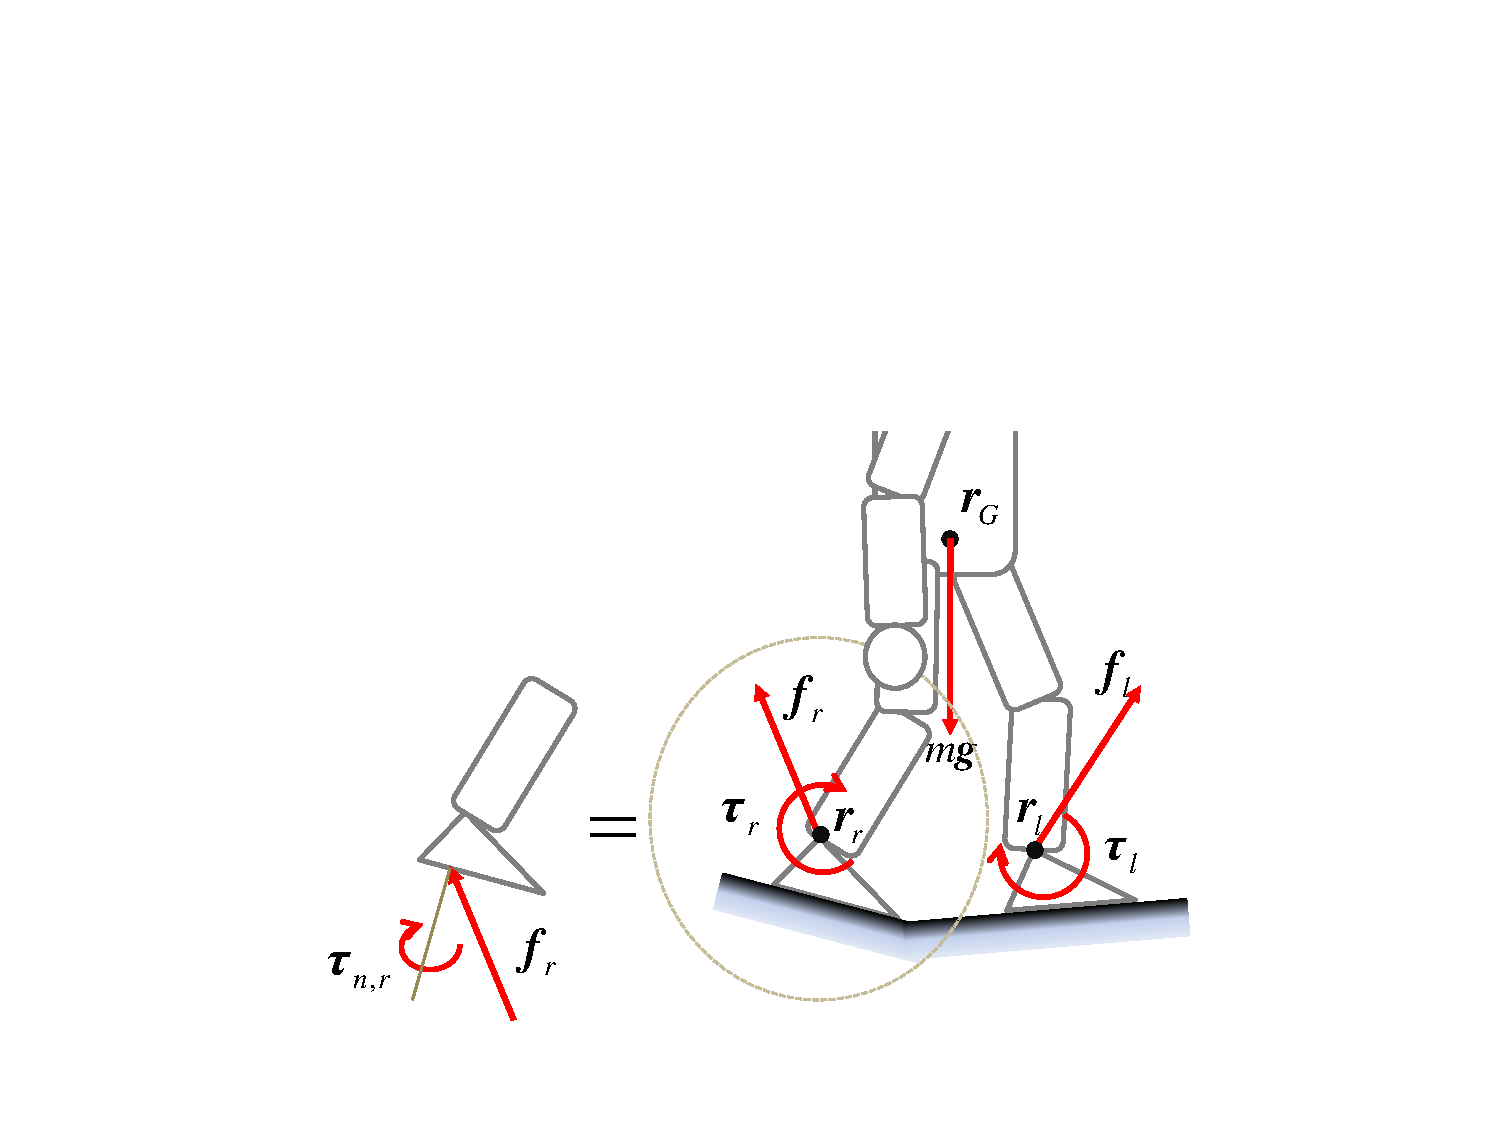
\includegraphics[width = 0.7\columnwidth]{Figures/double_support.pdf}
\end{center}
\caption{By expressing GRF applied to each foot with respect
to the local frame of the foot located at the ankle,
we can factor out the moments $\vtau_r$, $\vtau_l$ applied
to the ankle by the foot GRFs $\vf_r$ and $\vf_l$.
$\vr_r$ and $\vr_l$ are the positions of the ankles.}
\label{fig:double_support}
\end{figure}

The ankle torques $\vtau_i,~(i=r,l)$ are expressed in terms of
foot GRF and foot CoP as follows (Fig.~\ref{fig:foot}):
\begin{align}
	\vtau_i &= (\mR_i \vd_i) \times \vf_i + \mR_i\vtau_{n,i}  \, ,\label{eq:vmi}
\end{align}
where $\mR_i$ is the orientation of the foot, $\vd_i$ is the foot CoP in body frame,
and $\vtau_{n,i}=(0,0,\tau_{n,i})$ is the normal torque in body frame.

\begin{figure}
\begin{center}
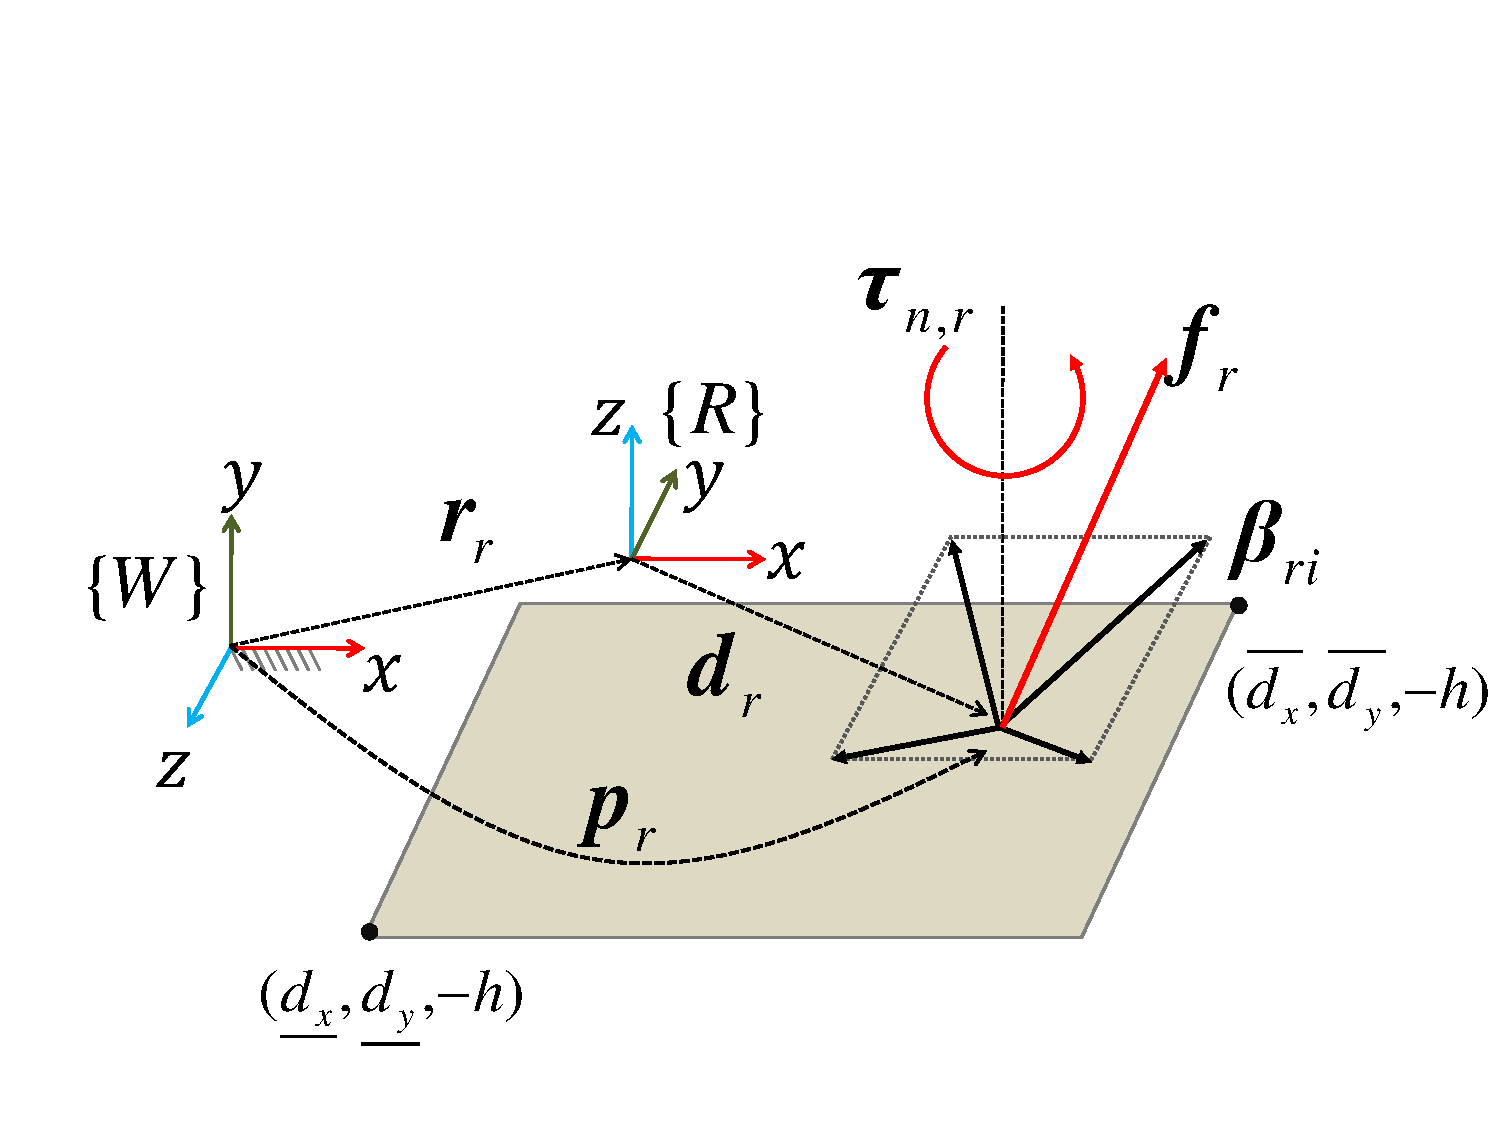
\includegraphics[width = 0.7\columnwidth]{Figures/foot_new.pdf}
\end{center}
\caption{We represent the foot/ground interaction forces on
the right foot using foot CoP, whose location with respect to
 the right
foot frame $\{R\}$ is denoted by $\vd_r=(\vd_{r,X},\vd_{r,Y},-h)$, ground reaction
moment normal to the ground $\vtau_{n,r}=(0,0,\tau_{n,r})$, and the GRF $\vf_r$.
%$\vf_r$ is represented using four basis vectors $\vbeta_{rj}~(j=1\ldots 4)$ that approximate the friction cone of the ground, i.e., $\vf_r=\sum_j \vbeta_{rj} \rho_{rj}$, where $\rho_{rj}~(\ge 0)$ is the magnitude in the direction of $\vbeta_{rj}$. Therefore, the ground pressure is defined by 7 parameters, $\left(\rho_{r1},\ldots,\rho_{r4},d_{r,X},d_{r,Y},\tau_{n,r}\right)$. This representation is compact, having only one more parameter than the minimum (3 for force and 3 for torque), and constraint can be expressed in a very simple form for a rectangular convex hull of the foot sole, i.e., $\rho_j\ge 0$, $\underline{d_j} \le d_j \le \overline{d_j}$, and $ |\tau_n| < \mu_\tau f_{r,N}$ where $f_{r,N}$ is the normal component of $\vf_r$, i.e., the Z-coordinate of $\mR_r^T\vf_r$ with $\mR_r$ being the orientation of the right foot. $\mu_\tau$ is a friction coefficient for torque and $h$ is the height of foot frame from the foot sole. Note that $\vd_r$ and $\vtau_{n,r}$ are expressed with respect to the body frame $\{R\}$ while $\vr_r$, $\vp_r$, $\vf_r$, and $\vbeta_{rj}$ are with respect to the world frame.
}
\label{fig:foot}
\end{figure}

Given $\vdk$ and $\vdl$, solving for foot GRFs and foot CoPs
is an underdetermined problem, which lets us prescribe additional optimality
criteria to find a solution.
If we incorporate minimal ankle torques into the optimality condition,
we could express the objective function as follows:
\begin{equation}
\begin{split}
	w_l ||\vdl_d - \vdl(\vf_r,\vf_l)||^2 + w_k ||\vdk_d - \vdk(\vf_r,\vf_l,\vtau_r,\vtau_l)||^2 \\
	+ w_f \left( ||\vf_r||^2+||\vf_l||^2 \right)
	+ w_\tau \left( ||\vtau_r||^2+||\vtau_l||^2 \right) \\
	\text{~s.t. $\vf_i$ and $\vtau_i$ are admissible}
\end{split}
\label{eq:opt_double}
\end{equation}
where the first two terms aim to achieve the desired momentum rate change,
the third term regularizes foot GRFs, and the last term tries to minimize ankle torques.
$w$'s are weighting factors among the different objectives.

Equation (\ref{eq:opt_double}) represents a nonlinear and non-quadratic
optimization problem and it especially contains nonlinear
cross product terms (see (\ref{eq:vmi})); this makes it difficult to use in a real-time controller. 
One solution is to convert this general nonlinear optimization problem
to easier ones that can be solved using least-squares or
quadratic programming methods. This can be achieved by
expressing the foot GRF and foot CoP
using the forces at certain specific locations on the boundary of the foot soles~\cite{Pollard01, Hyon07}.
However, this approach increases the dimension of the search space
significantly. %For example, \cite{Pollard01} used 16 variables to model the GRF and CoP of one foot, which is 10 more than the dimension of the unknowns.
Instead of increasing the search space to make the optimization problem
easier, we approximate (\ref{eq:opt_double}) with
two constrained least-squares problems, one for determining the foot GRFs, and
the other for determining the foot CoPs. This way the number
of variables is kept small.
Additionally, we attempt to minimize the ankle torques.
Minimizing ankle torques is meaningful because
large ankle torques can cause foot slipping.

This approach can be intuitively understood as follows.
In order to minimize the ankle torques ($\vdk_\tau\rightarrow\vzero$),
the foot GRFs $\vf_r$ and $\vf_l$ should create $\vdk_f$ as close to
the desired angular momentum rate change ($\vdk_f\rightarrow\vdk_d$) as possible while satisfying $\vdl_d$.
If $\vdk_f=\vdk_d$, the ankle torques can vanish.
If $\vdk_f\neq \vdk_d$, we compute the ankle torques that are necessary to generate
the residual angular momentum rate change, $\vdk_d-\vdk_f$.
In other words, by reducing burdens on the ankle torques to create $\vdk_d$,
it solves (\ref{eq:opt_double}) for the case in which minimizing ankle torques has higher priority
than regularizing foot GRFs.

\paragraph{Determination of Foot GRFs:}
In order to compute the foot GRFs,  $\vf_r$ and $\vf_l$, we solve the optimization problem below:
\begin{align}
	\min &|| \vdl_d - \vdl(\vf_r,\vf_l) ||^2 + w_k || \vdk_d - \vdk_f(\vf_r,\vf_l) ||^2 \nonumber \\ &+\epsilon_f ( || \vf_r ||^2 + || \vf_l ||^2 ) \, ,
\label{eq:opt_f}
\end{align}
where $w_k$ and $\epsilon_f~(w_k \gg \epsilon_f > 0)$
are weighting factors for angular momentum and
the regularization of foot GRFs, respectively.
Note that, if $\vdk_d = \vdk_f$, the ankle torques $\vtau_i$ become zero.
Each foot GRF is modeled using four basis vectors $\vbeta_{ij}$
and their magnitudes $\rho_{ij}$ that approximate the friction cone (an inverted
pyramid in Fig.~\ref{fig:foot}) on the ground
\begin{equation}
	\vf_i = \sum_{j=1}^4  \vbeta_{ij} \rho_{ij} := \vbeta_i \vrho_i  \, , \label{eq:pyramid}
\end{equation}
where $\vbeta_i=[\vbeta_{i1}~\cdots~\vbeta_{i4} ]$.



Note that $\vr_r$ and $\vr_l$ are determined by the configuration of the robot; they are constants when solving this problem. Therefore $\vdk_f$ becomes a
linear equation of $\vrho_i$ when we substitute (\ref{eq:pyramid}) into (\ref{eq:vdk_f}).  %(?? What is the significance of this sentence?).
Rearranging into a matrix equation, we can turn the optimization problem (\ref{eq:opt_f})  into a linear least-squares problem with non-negativity constraints where the only unknowns are the $\vrho_i$:
\begin{equation}
	\min || \mPhi \vrho - \vxi ||^2 \text{~s.t.~} \vrho_i \ge 0  \, ,\label{eq:nnls}
\end{equation}
where \footnote{
The vector $\vdelta_i$  expresses angular momentum
rate change (\ref{eq:vdk_f}) in terms of $\vrho_i$ as follows:
\begin{align*}
(\vr_r-\vr_G)\times\vf_r
%&= \sum_{j=1}^4 \left( (\vr_r-\vr_G)\times \vbeta_{r,j} \right) \rho_{r,j}
= (\vr_r-\vr_G)\times \left(\vbeta_r \vrho_r \right)
= \underbrace{\skewsym{ {\vr_i-\vr_G} }\vbeta_r}_{\vdelta_r} \vrho_r
&:= \vdelta_r \vrho_r
\end{align*}}
\begin{align}
	\mPhi &= \begin{bmatrix}
	\begin{matrix}
	\vbeta_r & \vbeta_l \\
	w_f\vdelta_r & w_f\vdelta_l
	\end{matrix}
	\\
	\epsilon_f \eye
	\end{bmatrix}\in \real^{(3+3+8)\times(4+4)} \\ 	
	\vxi &= \begin{bmatrix} \vdl_d-m\vg \\  w_f\vdk_d \\ \vec{0} \end{bmatrix} \in \real^{(3+3+8)}\nonumber\\
	\vrho &= \begin{bmatrix} \vrho_r^T & \vrho_l^T \end{bmatrix}^T \in \real^{8}\\
	\vdelta_i &= \skewsym{ {\vr_i-\vr_G} }\vbeta_i
\end{align}

\paragraph{Determination of Foot CoPs:}
In general, the desired angular momentum rate change cannot be fully generated
only by $\vf_r$ and $\vf_l$, so the residual, $\vdk_{\tau,d} = \vdk_d - \vdk_f$,
should be generated by
the ankle torques. To this end, we determine the location of each foot CoP such that
they create $\vdk_{\tau,d}$ while minimizing each ankle torque.
It is to be noted that, after having determined $\vf_i$, (\ref{eq:vmi}) can be written
as a linear function of $\vd_i$ and $\vtau_{n,i}$:
\begin{equation}
	\vtau_i = -\skewsym{\vf_i} \mR_i\vd_i + \mR_i\vtau_{n,i} \, ,
	\label{eq:vm_r}
\end{equation}
so that we can express
the optimization problem as a least-squares problem with upper and lower
bounds:

\begin{equation}
	\min || \mPsi \veta - \vkappa ||^2  \text{~s.t.~} \underline{\veta} \le \veta \le \overline{\veta}  \, ,\label{eq:opt_m}
\end{equation}
where
\begin{align}\label{eq:Psi}
	\mPsi &= \begin{bmatrix} \mPsi_k \\	\epsilon_p \eye \end{bmatrix}\in \real^{(3+6)\times 6}, ~	
	\vkappa = \begin{bmatrix} \vkappa_k \\ \epsilon_p \veta_d \end{bmatrix}\in \real^{(3+6)} \\
	\veta &=[ d_{r,X}~ d_{r,Y}~ \tau_{n,r} ~ d_{l,X} ~ d_{l,Y} ~ \tau_{n,l} ]^T\in \real^{6}  \, ,
\end{align}
where the elements of the constant matrix $\mPsi_k\in \real^{3\times 6}$ and $\vkappa_k$ are determined
from (\ref{eq:vm_r}).\footnote{Specifically, $\mPsi_k = [\mPsi_k^0 \ldots \mPsi_k^5]$ where
\begin{align*}
\mPsi_k^0 &= -\mR_{r}^1\vf^b_{r,Z} + \mR_{r}^2\vf^b_{r,Y},\quad \mPsi_k^1 = \mR_{r}^0\vf^b_{r,Z} - \mR_{r}^2\vf^b_{r,X},\quad \mPsi_k^2 = \mR_{r}^2,\\
\mPsi_k^3 &= -\mR_{l}^1\vf^b_{l,Z} + \mR_{l}^2\vf^b_{l,Y},\quad \mPsi_k^4 = \mR_{l}^0\vf^b_{l,Z} - \mR_{l}^2\vf^b_{l,X},\quad \mPsi_k^5 = \mR_{l}^2,
\end{align*}
and $\vkappa_k = \vdk_{\tau,d} + h ( \mR_{r}^1\vf^b_{r,X} - \mR_{r}^0\vf^b_{r,Y} + \mR_{l}^1\vf^b_{l,X} - \mR_{l}^0\vf^b_{l,Y} )$.
$\mR_{i}^j$ is $j$-th column vector of $\mR_i$ $(i=r,l)$, $\vf^b_i=\mR_i^T\vf_i$, and $h$ is the height of foot frame from the foot sole.
}

$\underline{\veta}$ and $\overline{\veta}$ are determined from foot geometry,
friction coefficient, and the normal component of foot GRF (see Fig.~\ref{fig:foot}).
$\veta_d$ is chosen such that $\vtau_i$ is zero, i.e., the line
of action of $\vf_i$ intersects the ankle. %We solve Eq. (\ref{eq:opt_m})
 %using the Levenberg-Marquardt method~\cite{lourakis04LM}. %, popular and reliable algorithm for nonlinear
%least squares problems, to solve this optimization but other methods
%tailored to box constrained linear least squares problem such as~\cite{Stark95}
%could be used as well.
Note that both the least-squares problems have a small number of variables, so
the optimization can be carried out quickly.
